% ==============================================================================
% tento soubor pouzijte jako zaklad
% this file should be used as a base for the thesis
% Autoři / Authors: 2008 Michal Bidlo, 2019 Jaroslav Dytrych
% Kontakt pro dotazy a připomínky: sablona@fit.vutbr.cz
% Contact for questions and comments: sablona@fit.vutbr.cz
%==============================================================================
% kodovani: UTF-8 (zmena prikazem iconv, recode nebo cstocs)
% encoding: UTF-8 (you can change it by command iconv, recode or cstocs)
%------------------------------------------------------------------------------
% zpracování / processing: make, make pdf, make clean
%==============================================================================
% Soubory, které je nutné upravit nebo smazat: / Files which have to be edited or deleted:
%   projekt-20-literatura-bibliography.bib - literatura / bibliography
%   projekt-01-kapitoly-chapters.tex - obsah práce / the thesis content
%   projekt-30-prilohy-appendices.tex - přílohy / appendices appendices in English
%==============================================================================
\documentclass[czech, zadani]{fitthesis} % bez zadání - pro začátek práce, aby nebyl problém s překladem
%\documentclass[english]{fitthesis} % without assignment - for the work start to avoid compilation problem
%\documentclass[zadani]{fitthesis} % odevzdani do wisu a/nebo tisk s barevnými odkazy - odkazy jsou barevné
%\documentclass[english,zadani]{fitthesis} % for submission to the IS FIT and/or print with color links - links are color
%\documentclass[zadani,print]{fitthesis} % pro černobílý tisk - odkazy jsou černé
%\documentclass[english,zadani,print]{fitthesis} % for the black and white print - links are black
%\documentclass[zadani,cprint]{fitthesis} % pro barevný tisk - odkazy jsou černé, znak VUT barevný
%\documentclass[english,zadani,cprint]{fitthesis} % for the print - links are black, logo is color
% * Je-li práce psaná v anglickém jazyce, je zapotřebí u třídy použít 
%   parametr english následovně:
%   If thesis is written in English, it is necessary to use 
%   parameter english as follows:
%      \documentclass[english]{fitthesis}
% * Je-li práce psaná ve slovenském jazyce, je zapotřebí u třídy použít 
%   parametr slovak následovně:
%   If the work is written in the Slovak language, it is necessary 
%   to use parameter slovak as follows:
%      \documentclass[slovak]{fitthesis}
% * Je-li práce psaná v anglickém jazyce se slovenským abstraktem apod., 
%   je zapotřebí u třídy použít parametry english a enslovak následovně:
%   If the work is written in English with the Slovak abstract, etc., 
%   it is necessary to use parameters english and enslovak as follows:
%      \documentclass[english,enslovak]{fitthesis}

% Základní balíčky jsou dole v souboru šablony fitthesis.cls
% Basic packages are at the bottom of template file fitthesis.cls
% zde můžeme vložit vlastní balíčky / you can place own packages here

% Kompilace po částech (rychlejší, ale v náhledu nemusí být vše aktuální)
% Compilation piecewise (faster, but not all parts in preview will be up-to-date)
% \usepackage{subfiles}

% Nastavení cesty k obrázkům
% Setting of a path to the pictures
%\graphicspath{{obrazky-figures/}{./obrazky-figures/}}
%\graphicspath{{obrazky-figures/}{../obrazky-figures/}}

%---rm---------------
\renewcommand{\rmdefault}{lmr}%zavede Latin Modern Roman jako rm / set Latin Modern Roman as rm
%---sf---------------
\renewcommand{\sfdefault}{qhv}%zavede TeX Gyre Heros jako sf
%---tt------------
\renewcommand{\ttdefault}{lmtt}% zavede Latin Modern tt jako tt

% vypne funkci šablony, která automaticky nahrazuje uvozovky,
% aby nebyly prováděny nevhodné náhrady v popisech API apod.
% disables function of the template which replaces quotation marks
% to avoid unnecessary replacements in the API descriptions etc.
\csdoublequotesoff



\usepackage{url}


% =======================================================================
% balíček "hyperref" vytváří klikací odkazy v pdf, pokud tedy použijeme pdflatex
% problém je, že balíček hyperref musí být uveden jako poslední, takže nemůže
% být v šabloně
% "hyperref" package create clickable links in pdf if you are using pdflatex.
% Problem is that this package have to be introduced as the last one so it 
% can not be placed in the template file.
\ifWis
\ifx\pdfoutput\undefined % nejedeme pod pdflatexem / we are not using pdflatex
\else
  \usepackage{color}
  \usepackage[unicode,colorlinks,hyperindex,plainpages=false,pdftex]{hyperref}
  \definecolor{hrcolor-ref}{RGB}{223,52,30}
  \definecolor{hrcolor-cite}{HTML}{2F8F00}
  \definecolor{hrcolor-urls}{HTML}{092EAB}
  \hypersetup{
	linkcolor=hrcolor-ref,
	citecolor=hrcolor-cite,
	filecolor=magenta,
	urlcolor=hrcolor-urls
  }
  \def\pdfBorderAttrs{/Border [0 0 0] }  % bez okrajů kolem odkazů / without margins around links
  \pdfcompresslevel=9
\fi
\else % pro tisk budou odkazy, na které se dá klikat, černé / for the print clickable links will be black
\ifx\pdfoutput\undefined % nejedeme pod pdflatexem / we are not using pdflatex
\else
  \usepackage{color}
  \usepackage[unicode,colorlinks,hyperindex,plainpages=false,pdftex,urlcolor=black,linkcolor=black,citecolor=black]{hyperref}
  \usepackage{minted}
  \definecolor{links}{rgb}{0,0,0}
  \definecolor{anchors}{rgb}{0,0,0}
  \def\AnchorColor{anchors}
  \def\LinkColor{links}
  \def\pdfBorderAttrs{/Border [0 0 0] } % bez okrajů kolem odkazů / without margins around links
  \pdfcompresslevel=9
\fi
\fi
% Řešení problému, kdy klikací odkazy na obrázky vedou za obrázek
% This solves the problems with links which leads after the picture
\usepackage[all]{hypcap}

% Informace o práci/projektu / Information about the thesis
%---------------------------------------------------------------------------
\projectinfo{
  %Prace / Thesis
  project={BP},            %typ práce BP/SP/DP/DR  / thesis type (SP = term project)
  year={2021},             % rok odevzdání / year of submission
  date=\today,             % datum odevzdání / submission date
  %Nazev prace / thesis title
  title.cs={Analýza aplikačních firewallů sociálních sítí},  % název práce v češtině či slovenštině (dle zadání) / thesis title in czech language (according to assignment)
  title.en={Analysis of Application Firewalls in Online Social Networks}, % název práce v angličtině / thesis title in english
  %title.length={14.5cm}, % nastavení délky bloku s titulkem pro úpravu zalomení řádku (lze definovat zde nebo níže) / setting the length of a block with a thesis title for adjusting a line break (can be defined here or below)
  %sectitle.length={14.5cm}, % nastavení délky bloku s druhým titulkem pro úpravu zalomení řádku (lze definovat zde nebo níže) / setting the length of a block with a second thesis title for adjusting a line break (can be defined here or below)
  %Autor / Author
  author.name={Radim},   % jméno autora / author name
  author.surname={Zítka},   % příjmení autora / author surname 
  %author.title.p={Bc.}, % titul před jménem (nepovinné) / title before the name (optional)
  %author.title.a={Ph.D.}, % titul za jménem (nepovinné) / title after the name (optional)
  %Ustav / Department
  department={UITS}, % doplňte příslušnou zkratku dle ústavu na zadání: UPSY/UIFS/UITS/UPGM / fill in appropriate abbreviation of the department according to assignment: UPSY/UIFS/UITS/UPGM
  % Školitel / supervisor
  supervisor.name={Filip},   % jméno školitele / supervisor name 
  supervisor.surname={Januš},   % příjmení školitele / supervisor surname
  supervisor.title.p={Ing. },   %titul před jménem (nepovinné) / title before the name (optional)
  supervisor.title.a={},    %titul za jménem (nepovinné) / title after the name (optional)
  % Klíčová slova / keywords
  keywords.cs={sociální sítě, automatický přístup, webscraping, aplikační firewall, Selenium, analýza chování. User-Agent.}, % klíčová slova v českém či slovenském jazyce / keywords in czech or slovak language
  keywords.en={social networks, automatic access, webscraping, application firewall, Selenium, behaviour analysis, User-Agent.}, % klíčová slova v anglickém jazyce / keywords in english
  %keywords.en={Here, individual keywords separated by commas will be written in English.},
  % Abstrakt / Abstract
  abstract.cs={ Práce popisuje způsoby, jak lze přistupovat na sociální sítě pomocí automatického robota, smysl tohoto přístupu a~důvody vedoucí k používání ochran před automatickými roboty. Cílem je analyzovat aktuálně používané ochrany před automatickými roboty nejznámějších sociálních sítí (Facebook, Twitter, LinkedIn a YouTube) a rozšířit tyto informace mezi ostatní vývojáře. Ti poté mohou využít těchto znalostí pro ochranu svých webových stránek. Výstupem této bakalářské práce je popis aktuálně používaných ochran a dále návrh ochrany, která pomáhá odhalit automatické roboty na základě podezřelého chování. }, % abstrakt v českém či slovenském jazyce / abstract in czech or slovak language
  abstract.en={The thesis describes ways to attend social networks using automatic robots, meaning of this approach and the reasons leading social networks to use protection against automated robots. The aim of this thesis is to analyze currently used protections against automatic robots of the most famous social networks (Facebook, Twitter, LinkedIn and Youtube). These informations are available for other developers, which may use these information to protect their own websites. The output of this bachelor thesis are description of currently used protections and proposal of protection that reveals automatic robots based on multiple identical behavior. }, % abstrakt v anglickém jazyce / abstract in english
  %abstract.en={An abstract of the work in English will be written in this paragraph.},
  % Prohlášení (u anglicky psané práce anglicky, u slovensky psané práce slovensky) / Declaration (for thesis in english should be in english)
  declaration={Prohlašuji, že jsem tuto bakalářskou práci vypracoval samostatně pod vedením pana Ing.~Filipa Januše.
Uvedl jsem všechny literární prameny, publikace a~další zdroje, ze kterých jsem čerpal.},
  %declaration={I hereby declare that this Bachelor's thesis was prepared as an original work by the author under the supervision of Mr. X
% The supplementary information was provided by Mr. Y
% I have listed all the literary sources, publications and other sources, which were used during the preparation of this thesis.},
  % Poděkování (nepovinné, nejlépe v jazyce práce) / Acknowledgement (optional, ideally in the language of the thesis)
  acknowledgment={ Děkuji panu Ing.~Filipu Janušovi za vedení této bakalářské práce. Vděčím mu zejména za jeho zájem, poskytnuté materiály, kvalitu konzultací a~všechny odpovědi na dotazy, které mě inspirovaly v tvorbě této práce. Dále děkuji Janu Švábíkovi za rady týkající se implementace této práce. },
  %acknowledgment={Here it is possible to express thanks to the supervisor and to the people which provided professional help
%(external submitter, consultant, etc.).},
  % Rozšířený abstrakt (cca 3 normostrany) - lze definovat zde nebo níže / Extended abstract (approximately 3 standard pages) - can be defined here or below
  %extendedabstract={Do tohoto odstavce bude zapsán rozšířený výtah (abstrakt) práce v českém (slovenském) jazyce.},
  %faculty={FIT}, % FIT/FEKT/FSI/FA/FCH/FP/FAST/FAVU/USI/DEF
  faculty.cs={Fakulta informačních technologií}, % Fakulta v češtině - pro využití této položky výše zvolte fakultu DEF / Faculty in Czech - for use of this entry select DEF above
  faculty.en={Faculty of Information Technology}, % Fakulta v angličtině - pro využití této položky výše zvolte fakultu DEF / Faculty in English - for use of this entry select DEF above
  department.cs={Ústav matematiky}, % Ústav v češtině - pro využití této položky výše zvolte ústav DEF nebo jej zakomentujte / Department in Czech - for use of this entry select DEF above or comment it out
  department.en={Institute of Mathematics} % Ústav v angličtině - pro využití této položky výše zvolte ústav DEF nebo jej zakomentujte / Department in English - for use of this entry select DEF above or comment it out
}

% Rozšířený abstrakt (cca 3 normostrany) - lze definovat zde nebo výše / Extended abstract (approximately 3 standard pages) - can be defined here or above
%\extendedabstract{Do tohoto odstavce bude zapsán výtah (abstrakt) práce v českém (slovenském) jazyce.}

% nastavení délky bloku s titulkem pro úpravu zalomení řádku - lze definovat zde nebo výše / setting the length of a block with a thesis title for adjusting a line break - can be defined here or above
%\titlelength{14.5cm}
% nastavení délky bloku s druhým titulkem pro úpravu zalomení řádku - lze definovat zde nebo výše / setting the length of a block with a second thesis title for adjusting a line break - can be defined here or above
%\sectitlelength{14.5cm}

% řeší první/poslední řádek odstavce na předchozí/následující stránce
% solves first/last row of the paragraph on the previous/next page
\clubpenalty=10000
\widowpenalty=10000

% checklist
\newlist{checklist}{itemize}{1}
\setlist[checklist]{label=$\square$}

\begin{document}
  % Vysazeni titulnich stran / Typesetting of the title pages
  % ----------------------------------------------
  \maketitle
  % Obsah
  % ----------------------------------------------
  \setlength{\parskip}{0pt}

  {\hypersetup{hidelinks}\tableofcontents}
  
  % Seznam obrazku a tabulek (pokud prace obsahuje velke mnozstvi obrazku, tak se to hodi)
  % List of figures and list of tables (if the thesis contains a lot of pictures, it is good)
  \ifczech
    \renewcommand\listfigurename{Seznam obrázků}
  \fi
  \ifslovak
    \renewcommand\listfigurename{Zoznam obrázkov}
  \fi
  % {\hypersetup{hidelinks}\listoffigures}
  
  \ifczech
    \renewcommand\listtablename{Seznam tabulek}
    \renewcommand{\lstlistingname}{Code}
  \fi
  \ifslovak
    \renewcommand\listtablename{Zoznam tabuliek}
  \fi
  % {\hypersetup{hidelinks}\listoftables}

  \ifODSAZ
    \setlength{\parskip}{0.5\bigskipamount}
  \else
    \setlength{\parskip}{0pt}
  \fi

  % vynechani stranky v oboustrannem rezimu
  % Skip the page in the two-sided mode
  \iftwoside
    \cleardoublepage
  \fi

  % Text prace / Thesis text
  % ----------------------------------------------
  \ifenglish
    \input{projekt-01-kapitoly-chapters-en}
  \else
    % Autoři: Michal Bidlo, Bohuslav Křena, Jaroslav Dytrych, Petr Veigend a~Adam Herout 2019
\chapter{Úvod}

Automatický přístup na sociální sítě znamená přístup na webové stránky pomocí automatického bota, jehož chování na webové stránce je předem definováno (na rozdíl od chování lidské osoby). Automatický přístup slouží k~získávání dat z~webových serverů, mezi něž pochopitelně patří i~sociální sítě. Existuje mnoho podnětů proč používat automatický přístup~--~může jít například o~získání a~následné zpracování určitých vyžádaných dat. Ta se mohou týkat například lidí nebo produktů, o~kterých tvůrce robota potřebuje zjistit určitá data (chování, zájmy apod.), a~následně je použít pro svoje konkrétní účely. Sociální sítě mají mnoho důvodů, proč bránit automatickým botům v~přístupu na jejich stránky, mezi něž patří například šíření SPAMu. Sociální sítě by měly mít pokročilou ochranu proti automatickému přístupu a~právě proto je vhodné tyto ochrany studovat právě na sociálních sítích.

Tato bakalářská práce se zabývá ochranou proti automatickému přístupu na web, proto je nezbytné pochopit základní principy webové komunikace, které jsou popsány v~kapitole~\ref{chap:web_communication}. Kapitola~\ref{chap:network_protection} je věnována ochranám na síťové a~transportní vrstvě a~dále popisuje útoky na tyto vrstvy. Způsoby, pomocí nichž lze implementovat automatický přístup, obsahuje kapitola~\ref{chap:auto_approach_to_web}. Hlavní cíl práce je detekce aktuálně používaných opatření, která používají sociální sítě pro rozpoznání automatického robota. Tyto metody jsou popsány v~kapitole~\ref{chap:application_firewall} a~mohou sloužit ostatním vývojářům jako inspirace pro ochranu jejich webových serverů. 

Implementační část práce (kapitola~\ref{chap:proposal_of_solution}) popisuje navržený způsob ochrany proti automatickému přístupu. Řešení simuluje reálnou sociální síť, kde jednotliví uživatelé sdílejí svoje znalosti či myšlenky. Je implementována v~jazyce NodeJS s~využitím databáze MongoDB. Navržená ochrana spočívá v~detekci identického chování uživatele v~určitém časovém intervalu a~dalších podezřelých a~neobvyklých aktivit.

Cílem této práce je pomoci vývojářům v~získávání vědomostí o~použití ochran proti automatickým robotům, které mohou následně implementovat na svoje webové stránky. Pomocí funkční ochrany lze zachovat soukromí svých uživatelů a~bezpečnost dat. Dalším důvodem k~vylepšování ochrany je zabránění šíření nežádoucího spamu či psaní nevhodných komentářů. Současně používané techniky, které využívají automatičtí roboti, jsou velmi pokročilé a~odhalit automatický přístup se stává těžkým úkolem.

\chapter{Webová komunikace}
\label{chap:web_communication}
V této kapitole jsou čtenáři objasněny některé základní pojmy týkající se webové komunikace. Tyto znalosti jsou nezbytné pro funkční nastavení automatického bota\footnote{Pojmem bot je myšlen automat, který automaticky přistupuje na webové stránky.} tak, aby ochrana webového serveru (tzn. firewally nižších vrstev a aplikační firewall, kapitoly~\ref{chap:network_protection} a~\ref{chap:application_firewall}) neodhalila podezřelý provoz a~naopak~--~aby bylo možné analyzovat podezřelý webový provoz z~pohledu vlastníka serveru.

\section{Protokol HTTP/HTTPS}
\label{sec:http}
Protokol je v~informatice sada pravidel. HTTP protokol definuje pravidla, podle kterých probíhá datový tok mezi klientem a~serverem. Pomocí HTTP protokolu lze navštěvovat různé webové stránky. HTTP spojení začíná vždy klientská strana komunikace. Nástroj, který komunikuje na klientské straně se serverem se nazývá \texttt{User-Agent}. \texttt{User-Agent} představuje zpravidla \textit{webový prohlížeč}~\ref{sec:web_browser}, ale může to být i~jiný nástroj.
Při návštěvě webové stránky vytvoří \texttt{User-Agent} HTTP dotaz. Poté tento dotaz pošle na dotazovaný server, který obsahuje webovou stránku, a~následně obdrží odpověď obsahující data (příklad HTTP komunikace na obr.~\ref{img:HTTP_request}). S~těmito daty může \texttt{User-Agent} naložit dle vlastního uvážení. Webový prohlížeč z~těchto dat sestavuje webovou stránku tak, aby byla čitelná pro uživatele (klienta). V~případě, že \texttt{User-Agent} není webový prohlížeč, může se jednat o~automatický přístup na server.

Klasické HTTP přenášelo data po síti nešifrovaně, takže si je mohl přečíst útočník, který v~jakémkoliv bodě na lince odposlouchával přenos. Z~tohoto důvodu vznikl protokol HTTPS, který zajišťuje šifrované spojení.

V rámci HTTP dotazu je nutné nějakým způsobem přenášet data od klienta na server. K~tomu slouží metody GET a~POST~\cite{bib:httpRFC}. 

\begin{figure}[hbt]
	\centering
	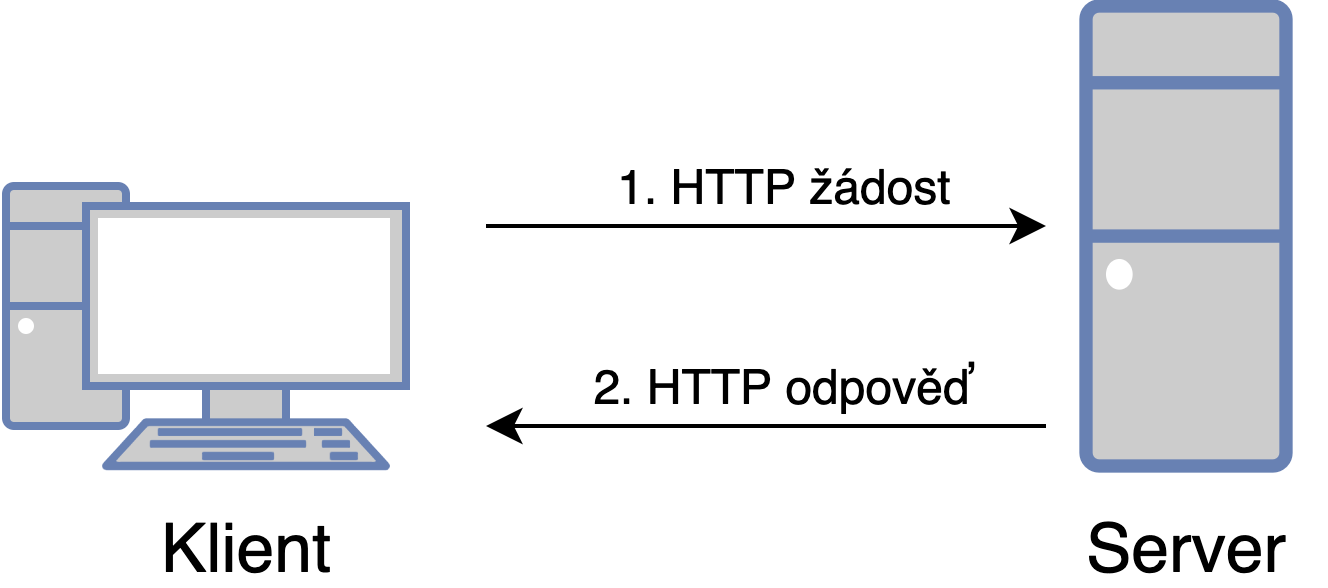
\includegraphics[width=0.6\textwidth]{images/HTTP_request.png}
	\caption{Jednoduchá HTTP komunikace mezi dvěma uzly}
	\label{img:HTTP_request}
\end{figure}

\subsection*{Metoda GET}
Metoda GET využívá pro přenos dat URI požadovaného dokumentu. Pokud na webový server dojde požadavek ve tvaru: \texttt{GET /en-US/docs/Web/HTTP/ HTTP 1.1}, server ví, že tato koncová stanice žádá stránku odpovídající adrese \texttt{/en-US/docs/Web/HTTP/}. V~tomto dotazu se však mohou nacházet další parametry, pokud se za touto cestou nachází znak otazníku. Ty obsahují nějaké další informace, které chce klient sdělit serveru. Jde například o~data z~formuláře a~má tvar: \texttt{?query=hledaný+výraz}. V~tomto případě proměnná \texttt{query} obsahuje výraz \uv{hledaný výraz}.

\subsection*{Metoda POST}
Metoda POST slouží ke~stejnému účelu jako metoda GET. Pomocí této metody může uživatel posílat objemnější množství dat na webový server. Odeslaná data mají stejný formát, avšak proti metodě GET se liší tím, že tato data posílá jako součást HTTP dotazu a~nejsou tedy jednoduše viditelná v~URI adrese. 

\subsection*{HTTP hlavička}
HTTP hlavička obsahuje metadata k~odeslaným nebo přijatým datům. V~dotazu HTTP hlavičky jsou informace jako je metoda, URL požadované stránky, IP adresa vzdáleného serveru, číslo portu, jazyk, čas vytvoření požadavku, informace o~cookies, \texttt{User-Agent} (podrobněji níže) atd.

Automatický přístup často v~HTTP hlavičce poskytuje pouze nejnutnější informace, čímž se stává jednodušeji odhalitelný. \uv{Ruční} úprava či vyplnění dalších informací v~hlavičce HTTP dotazu může vést k~úspěšnému překonání aplikačního firewallu.

\subsection*{User-Agent}
\label{sec:user_agent}
Hlavička HTTP dotazu obsahuje několik informací, z~nichž jedna je právě \texttt{User-Agent}~(UA). Kvalitní webový prohlížeč dokáže poskytnout základní informace o~svém systému pro účely optimalizace webové stránky. Typickým použitím je přehrávání videa ve vysoké kvalitě, které zvládnou přehrát pouze výkonnější koncové stanice. Tyto informace se přenáší prostřednictvím \texttt{User-Agent} hodnoty. \texttt{User-Agent} zahrnuje informace o~systémových písmech, pluginech, verzi prohlížeče, CPU apod. Typický obsah UA má podobu: \texttt{Mozilla/5.0 (Macintosh; Intel Mac OS X 11\_0\_0) AppleWebKit/537.36 (KHTML,
\\
like Gecko) Chrome/86.0.4240.183 Safari/537.36}.

\section{Webový prohlížeč}
\label{sec:web_browser}
Webový prohlížeč je aplikace, který na základě uživatelských příkazů komunikuje s~určitým webovým serverem (viz protokol HTTP~\ref{sec:http}). Data, která získává touto komunikací, vykresluje jako webovou stránku podle přesně definovaných pravidel (viz~\ref{sec:html}). Webový prohlížeč si ukládá data o~navštívených stránkách, tzv.~cookies~\ref{sec:cookies}. Při procházení jednotlivých stránek si může mimo cookies ukládat i~obsah stránek do cache za účelem rychlejšího načítání v~budoucnosti.

V moderních prohlížečích existují nástroje \footnote{Pro prohlížeče pracující s~jádrem Google Chrome se tento nástroj nazývá Chrome DevTools.}, pomocí nichž je možné jednoduše upravovat celou webovou stránku (HTML dokument), připojit se na konzoli a~pracovat s~JavaScriptovým obsahem apod. Tento nástroj také umožňuje sledovat síťový provoz dané webové stránky a~poté jej analyzovat. Znalost získanou analýzou provozu lze využít pro naprogramování automatického bota, který poté může velmi dobře simulovat běžný uživatelský provoz~\cite{bib:google_inspect}.

\subsection*{Browser fingerprint}
\label{sec:browser_fingerprint}
Browser fingerprinting, (volně přeloženo \textit{\uv{otisk prstu prohlížeče}}) je trackovací technika, která identifikuje jednotlivé uživatele na základě poskytnutých informací v~HTTP hlavičce. Aby se mohla webová stránka zobrazit korektně, tak webový server žádá tyto informace (rozlišení obrazovky, operační systém, jazyková nastavení apod.) a~pomocí nich ukládá Browser fingerprint daného uživatele. Pochopitelně může docházet ke~shodám, kdy jeden uživatel má identický fingerprint jako jiný uživatel, ale to se spíše jedná o~výjimku~\cite{bib:browser_fingerprint}.

V tabulce~\ref{tab:fingerprint_chrome} je znázorněn příklad otisku prstu prohlížeče. V~pravém sloupci je uveden počet procent uživatelů, kteří mají stejnou hodnotu jako je uvedená v~tabulce. Test byl proveden na stránce \href{https://amiunique.org/fp}{https://amiunique.org/fp}. Hodnota, která se liší nejvíce, je hodnota \texttt{User-Agent}. V~kombinaci s~ostatními hodnotami a~IP adresou lze s~poměrně velkou pravděpodobností rozpoznat jednoho určitého uživatele.

\begin{table}[ht]
  \begin{tabularx}{\linewidth}{
    |>{\hsize=0.5\hsize}X|% Vlastnost
    >{\hsize=2.0\hsize}X|% Hodnota
    >{\hsize=0.5\hsize}X|% Poměr procent
  }
    \hline
    \multicolumn{1}{|c|}{\textbf{Vlastnost}}& \multicolumn{1}{c|}{\textbf{Hodnota}} & \multicolumn{1}{c|}{\textbf{Poměr \%}} \\ \hline
    User-Agent & Mozilla/5.0 (Macintosh; Intel Mac OS X 10\_15\_7)
    AppleWebKit/537.36 (KHTML, like Gecko) Chrome/90.0.4430.93 Safari/537.37 & \textless{}0,01~\% \\ \hline
    Accept & text/html, application/xhtml+xml, application/xml; q=0.9,image/avif, image/webp,image/apng, */*;q=0.8,application/signed-exchange;v=b3;q=0.9 & 9,82~\% \\ \hline
    Content encoding & gzip, deflate, br & 79,65~\% \\ \hline
    Content language & en-GB,en-US;q=0.9,en;q=0.8 & 1,77~\% \\ \hline
    Referer & https://www.google.com & 0.32~\% \\ \hline
    \end{tabularx}

\label{tab:fingerprint_chrome}
\caption{Ukázka fingerprintu prohlížeče Google Chrome a~procentuální poměr webových prohlížečů, které používají stejnou hodntou}
\end{table}

\subsection*{Chrome DevTools}
\label{sec:chrome_devtools}
Nástroj Chrome DevTools je sada nástrojů pro webové vývojáře, který umožňuje velmi rychle upravovat webovou stránku přímo v~prohlížečích postavených na jádře Google Chrome. Těmito nástroji můžeme libovolně měnit vizuální vzhled stránky (uzly DOM stromu, CSS styly apod.), upravovat rozlišení displeje, zkoumat síťový provoz, vytížení paměti a~výpočetní kapacity stanice, spravovat cookies aptd. Slouží k~optimalizaci webových aplikací a~hledání chyb.

Díky zobrazení zdrojového HTML dokumentu v~Chrome DevTools lze identifikovat jednotlivé oblasti stránky, což lze využít například pro naprogramování automatických testů či sledovat změny HTML/CSS identifikátorů. Ukázka nástroje ChromeDevTools je zobrazena na obrázku~\ref{img:chrome_devtools}. Nástroj Chrome DevTools se spouští v~prohlížečích s~jádrem Chromium \textit{kliknutím pravého tlačítka myši~→~Inspect}.

\begin{figure}[hbt]
	\centering
	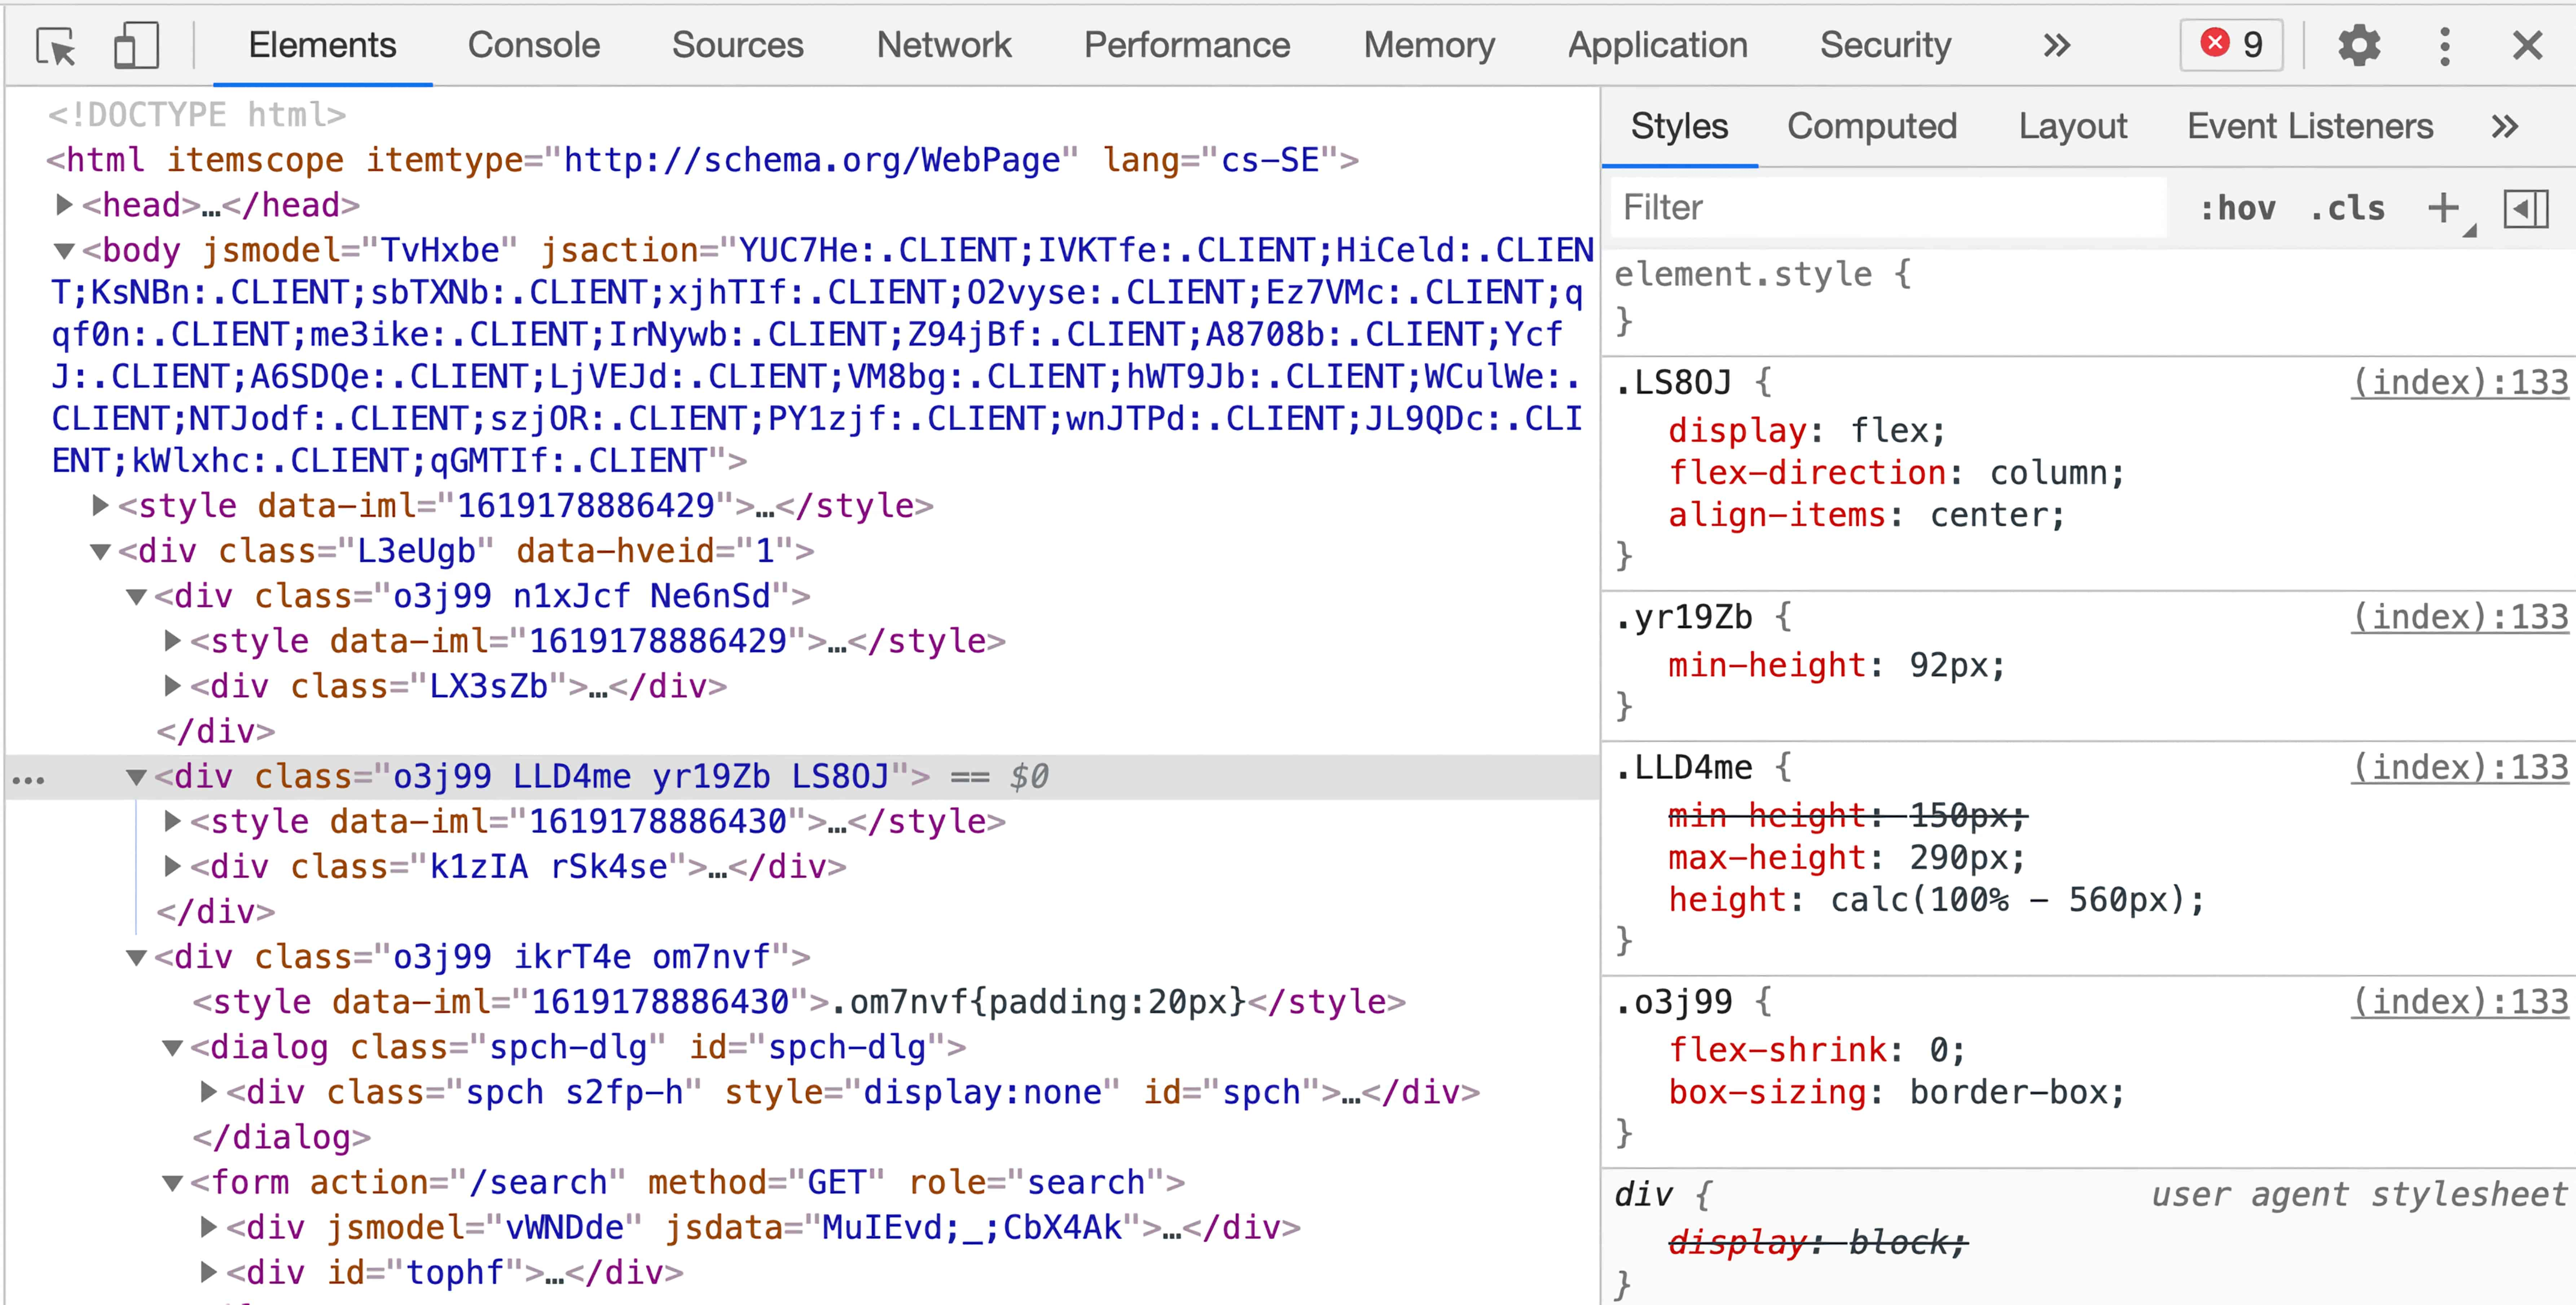
\includegraphics[width=0.95\textwidth]{images/chrome_devtools.jpg}
	\caption{Chrome DevTools}
	\label{img:chrome_devtools}
\end{figure}

\section{Anonymizační systém Tor}
\label{sec:tor_browser}
Síť Tor slouží k~anonymizaci uživatelů, tedy slouží k~ochraně jejich soukromí. Je udržována neziskouvou organizací \textit{The Tor project} a~veškerý zdrojový kód sítě Tor je open source. Nejvíce je využíván pro účely prohlížeče, jehož používáním získá uživatel téměř dokonalou anonymitu. Prohlížeč pro síť Tor se nazývá \textit{TorBrowser}~\cite{bib:tor_browser}. Může být využíván pro nelegální aktivity a~umožňuje přístup do Dark Webu.

Princip sítě Tor funguje na principu tunelování na Tor síti, tzv.~Onion routing. To zajišťuje, že veškerý provoz mezi klientem a~serverem je šifrovaný (což je standard v~dnešní době i~bez použití Toru), nicméně jeho hlavní přednost spočívá v~tom, že provoz je směrován přes více různých Tor serverů. Ty pak vystupují jako klient a~zajistí původnímu klientovi takřka naprostou anonymitu. Pro účely této práce je nejdůležitější, že klient vystupuje pokaždé pod jinou adresou a~velmi pravděpodobně z~jiného místa (např.~Londýn či New York). IP adresy, pod kterými klient vystupuje, jsou velmi často v~gray listu\footnote{Gray list je seznam IP adres, ze~kterých byl dříve zaznamenán podezřelý provoz či jsou nějakým jiným způsobem podezřelé. Více v~kapitole~\ref{sec:gray_list}.}, nicméně tyto adresy se neustále mění. 

Rozpoznat Tor adresu není příliš složité. Jde například o~nestandardní čísla portů, neexistující SSL vydavatel certifikátu, neexistující vydavatel certifikátu pro DNS apod.~\cite{bib:tor_recognition}.

\section{Cookies}
\label{sec:cookies}
Název cookies (přeloženo \textit{\uv{sušenka})} byl odvozen z~jeho původního významu. Při používání určitého webu se „pečou“ určitá data, která se ukládají právě do souborů cookies. Jsou to malé kusy dat, které obsahují data o~proběhlých návštěvách různých webů. Usnadňují práci s~webem, protože jednou nastavené údaje není nutné vyplňovat při každém přístupu znovu. Ukládají se do nich přihlašovací údaje (proto některé weby přihlašují uživatele automaticky), zvolený design stránky, obsah nákupního košíku apod.
Soubory cookies jsou velmi důležité pro automatický přístup na webové servery. Pokud umí automatický robot správně pracovat s~cookies, bude působit méně podezřele při dalších přístupech~\cite{bib:developerMozilla}.

\subsection*{Vznik cookies}
Pro automatický přístup je velmi důležité vědět, jak cookies vznikají. Při návštěvě stránky, která ještě nebyla uživatelem navštívena, resp. v~souborech cookies neexistuje cookies pro danou stránku, není přítomen v~HTTP žádosti atribut \texttt{cookies}. Server při vytváření odpovědi zahrne do HTTP odpovědi atribut (jeden či více) \texttt{Set-cookie} obsahující cookies, které se mají uložit do webového prohlížeče.

\subsection*{Doménová jména v~cookies}
Každá cookies musí obsahovat z~podstaty věci informace o~doméně, pro kterou dané cookies patří. Při návštěvě webové stránky hledá webový prohlížeč cookies patřící navštěvované doméně. Doménové jméno se nachází v~poli \texttt{Domain}. Doméně \textit{https://vutbr.cz/} bude odpovídat cookies, které obsahuje \texttt{Domain=vutbr.cz}. Avšak toto cookies bude uvažováno i~v případě návštěvy \textit{https://merlin.fit.vutbr.cz/}. Cookies často obsahuje atribut \texttt{Path}, který specifikuje místa na webovém serveru, při jejichž návštěvě se má toto cookies použít. Pro výše uvedenou doménu by se cookies s~atributem \texttt{Path} nabývající hodnotu \texttt{/studuj} použilo pouze v~případě návštěvy stránky \textit{https://vutbr.cz/studuj/}.

\section{Session}
\label{sec:session}
Data, se kterými uživatel pracuje na dané webové stránce, je poměrně nepohodlné a~nebezpečné ukládat do uživatelského cookies (\ref{sec:cookies}) nebo je přenášet po síti od uživatele na server. Z~tohoto důvodu se využívá HTTP session (překlad: \textit{\uv{relace}}). Klientské straně žádající přístup na server je přiřazen jednoznačný identifikátor (tzv.~\textit{JSESSIONID}), který je uložen v~cookies a~který jednoznačně identifikuje uživatelská data na serveru (čas přihlášení, počet přihlášení apod.). Při práci s~daty uživatel a~server pracují pouze s~tímto identifikátorem. Uživatel se autentizuje zpravidla uživatelským jménem a~heslem.

\subsection*{Tabulka s~informacemi o~sessions}
V tabulce~\ref{tab:session_cookie} je ukázka, jak mohou být uložena data o~sessions na straně serveru. Každý server může ukládat velké množství jakýchkoli informací, které potřebuje či může v~budoucnu potřebovat.

\begin{table}[H]
\centering
\label{tab:session_cookie}
\begin{tabular}{|c|c|c|c|}
\hline
\texttt{JSESSIONID} & \texttt{username} & \texttt{data} & \texttt{lastAccess} \\ \hline
A6CC39D2A106BAE4 & radimzitka & 78ha4d397ab & 2020-12-02 \\ \hline
76HE239B6D9CAA83& jansvabik & 76e3a9cca40 & 2019-12-28 \\ \hline
\end{tabular}
\caption{Uložená data o~relacích na straně serveru}
\end{table}

\subsection*{Vytvoření session}
\begin{enumerate}
  \item Klient vytvoří první HTTP žádost a~pošle ji na webový server.
  \item Webový server (resp. proces, který se stará o~sessions) vytvoří HTTP session pro klienta a~vygeneruje JSESSIONID, které uloží do cookies.
  \item Odpověď včetně vytvořeného cookies je zaslána zpět klientovi a~HTTP spojení je zrušeno.
  \item Session cookie k~webové stránce je uloženo ve webovém prohlížeči na klientské straně~\cite{bib:session_creating}.
\end{enumerate}

\begin{figure}[hbt]
	\centering
	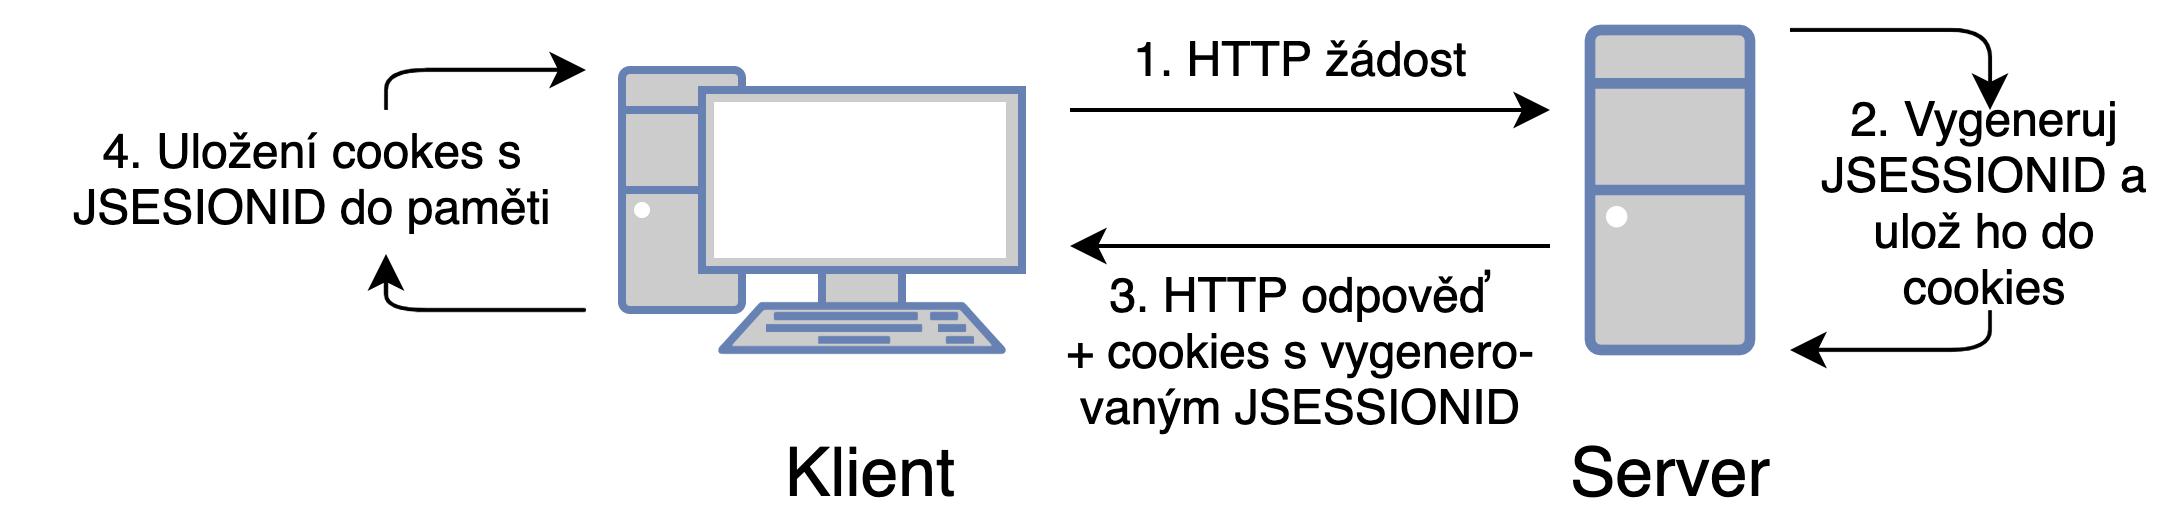
\includegraphics[width=0.6\textwidth]{images/cookie.png}
	\caption{Průběh vygenerování JSESSIONID}
	\label{img:session_ID_generate}
\end{figure}

\subsection*{Žádost o~přístup na stránku s~existujícím session ID}
\begin{enumerate}
  \item Klientský webový prohlížeč zažádá o~přístup na stránku, přičemž do žádosti přidá cookies, které získal v~předchozích spojeních.
  \item Webový server obdrží žádost s~existujícím session ID. Najde objekt odpovídající dané session v~paměti serveru a~zpracuje danou žádost s~použitím dat uložených v~nalezeném objektu.
  \item Webový server vytvoří odpověď a~zašle ji zpět na klientskou stranu~\cite{bib:session_connection}.
\end{enumerate}

\begin{figure}[hbt]
	\centering
	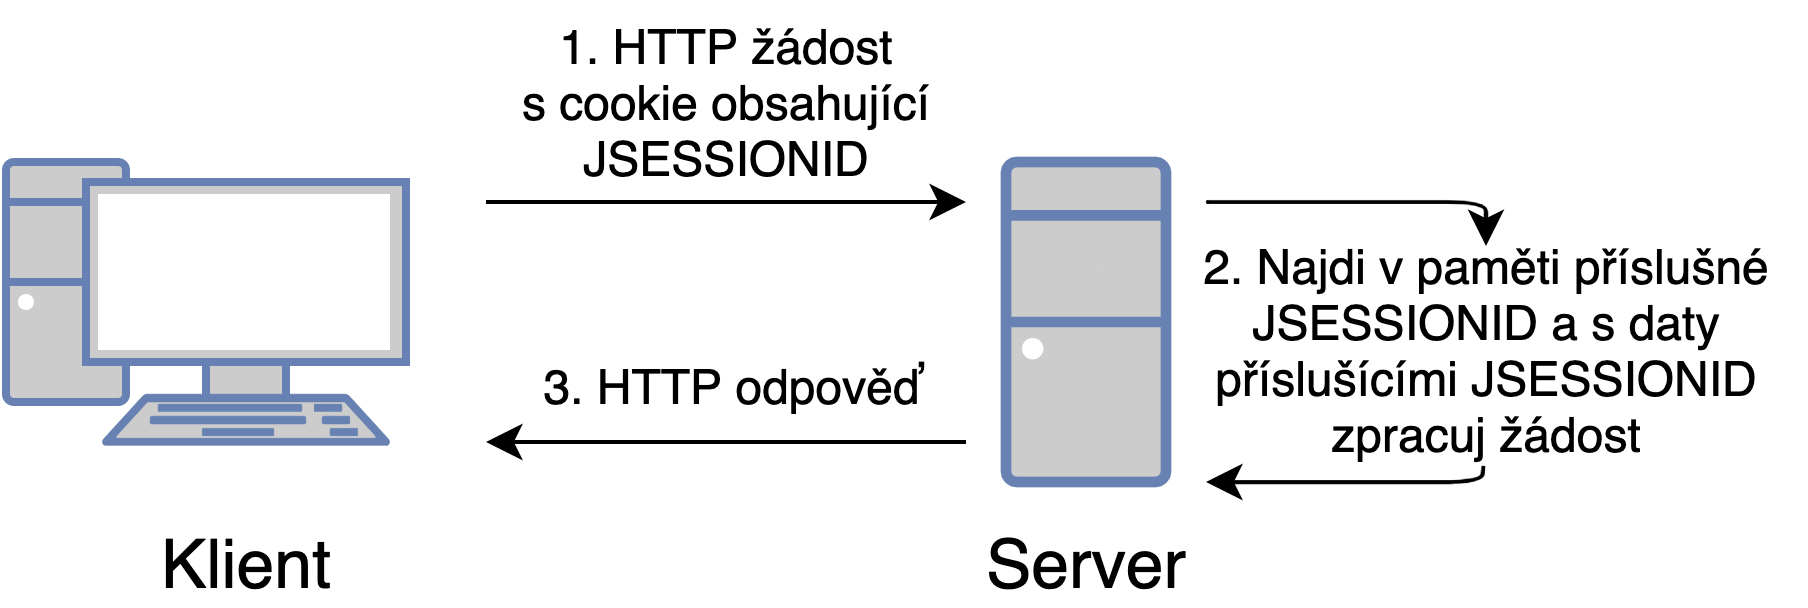
\includegraphics[width=0.6\textwidth]{images/cookie_repeat.png}
	\caption{Komunikace s~již existujícím JSESSIONID}
	\label{img:session_ID_created}
\end{figure}


\section{HTML}
\label{sec:html}
Značkovací jazyk HTML slouží pro popis webové stránky. HTML jazyk si klade za cíl, aby konečný vzhled popisované stránky nebyl ovlivněn parametry zařízení, na kterém je zobrazována. To znamená, že se webová stránka zobrazí ve velmi podobném designu jak na zařízení s~malým displejem, tak na zařízení disponujícím velkým displejem. Jazyk vychází ze~značkovacího jazyka SGML (viz \href{https://tools.ietf.org/html/rfc1874}{RFC SGML}), který je ale příliš komplikovaný pro využití v~kódování webových stránek. Pro účely automatického přístupu je klíčová znalost jazyka HTML, jelikož program, který simuluje webový prohlížeč, stahuje určitou HTML stránku. Z~ní poté extrahuje předem definovaná data nebo s~ní jinak pracuje, ale veškerá tato práce se většinou řídí HTML tagy~\cite{bib:htmlRFC}.

\subsection*{Popis jazyka}
Jazyk HTML je množina tagů (značek), kde každý jeden tag může obsahovat atributy (vlastnosti), které nabývají různých hodnot. Každá HTML značka má jednoznačný účel. Tagy se dělí na párové a~nepárové. Počet párových tagů v~dokumentu musí být vždycky sudý. Typickým představitelem párové HTML značky je \texttt{<html>}, k~němuž existuje dále v~dokumentu stejný tag označený lomítkem, např.~\texttt{</html>}. Nepárové tagy typicky nepokrývají žádnou oblast dokumentu. Zástupce nepárového tagu je znak nového řádku \texttt{<br>}.

Každý tag může mít určené svoje chování, které by mělo být definováno v~příslušném dokumentu, který popisuje kaskádové styly stránky. Jde například o~párový tag \texttt{<div>}, jehož atributem je identifikátor \texttt{id} a~nabývá hodnoty \texttt{link-like-feed-f5x3}. Každý prvek s~identifikátorem by měl být v~HTML dokumentu jedinečný a~díky tomu lze identifikovat akci (např.~kliknutí), kterou uživatel provádí na stránce. S~identifikátory HTML elementů pracuje aplikační firewall v~implementační části, pomocí nichž rozeznává elementy, na které bylo uživatelem kliknuto.

\section{JavaScript}
\label{sec:java_script}
JavaScript (JS) je nejznámější skriptovací jazyk pro webové stránky, který využívá mnoho dalších prostředí (Node.js, Adobe Acrobat). Společně s~jazyky HTML a~CSS tvoří jádro technologie WWW~\cite{bib:js_html_css}. Javascript provádí kód ve webovém prohlížeči (tedy na straně uživatele).

S použitím jazyka JS je možno prakticky ihned reagovat na vstup uživatele, umožňuje tedy měnit HTML prvky (popř.~je vytvářet), pracovat s~jejich obsahem či designem. JS umožňuje reagovat na pohyb myši, kliknutí na grafický prvek nebo v~reálném čase změnit hodnotu čísla či textu. Dále umožňuje práci s~webovým prohlížečem jako je pohyb v~historii a~otevírání či zavírání oken. Kód JavaScriptu se vykonává v~okamžiku, kdy na něj prohlížeč při procházení stránky narazí~\cite{bib:IIS_JS}.

V JavaScriptu je napsáno poměrně velké množství desktopových aplikací pomocí frameworku Electron. Mezi tyto aplikace patří např.~vývojové prostředí Visual Studio Code, chatovací programy Slack či Discord a~Skype~\cite{bib:electron}.

\chapter{Firewally nižších vrstev}
\label{chap:network_protection}
Kapitola se věnuje ochraně sítí na nižších vrstvách než je aplikační. Popisuje ochrany používané na těchto vrstvách a~dále se zabývá různými útoky na nižší vrstvy. Každému serveru nebo stanici v~síti hrozí jisté nebezpečí, že budou cílem útoku z~vnější sítě. Důvodů útočit na nějaké zařízení může být mnoho (krádež citlivých dat či hesel nebo odstávka sítě) a~je třeba jej chránit. Mnoho firem investuje nemalé částky pro ochranu svých dat a~zařízení, protože v~případě úspěšného útoku by následky mohly mít fatální dopad. Následující kapitola~\ref{chap:application_firewall} věnující se aplikačními firewallu využívá získané znalosti z~této kapitoly a~úzce na tuto kapitolu navazuje.

\section{Firewall}
Brána firewall je zařízení či soustava zařízení, která určitým způsobem kontroluje komunikaci mezi zařízením v~interní sítí a~zařízením ve vnější síti za účelem ochrany vnitřní sítě. Historie firewallu sahá až do roku 1987, kdy se instituce pracující s~citlivými informacemi začaly starat o~důvěrnost svých dat. Hlavní myšlenka byla postavit jakousi bránu mezi zdánlivě bezpečnou interní síť a~externími sítěmi. Dnešní firewally jsou často implementovány na lokální stanici v~podobě antivirového programu. V~rozsáhlejších (např.~korporátních) LAN sítích představují firewall samostatná síťová zařízení, přes která teče veškerá komunikace s~externími sítěmi. Role firewallu v~síti je znázorněna na obrázku~\ref{img:firewall}.

\begin{figure}[hbt]
	\centering
	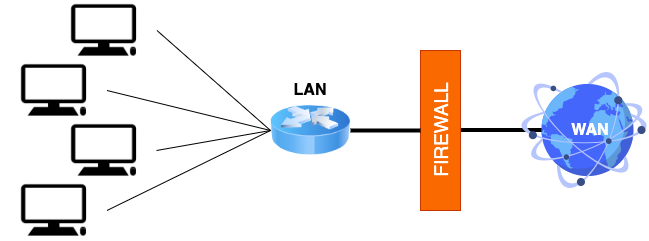
\includegraphics[width=0.6\textwidth]{images/firewall.png}
	\caption{Schéma fungování firewallu}
	\label{img:firewall}
\end{figure}

\noindent
S postupem času se firewall vyvíjel a~jeho druhy lze různě rozdělit v~závislosti na vlastnostech každého z~nich. V~této práci jsou rozděleny~\cite{bib:firewall} do tří velkých skupin: 

\begin{itemize}
	\item Paketové filtry
	\item Stavové filtry
	\item Aplikační brány\footnote{Protože se tato kapitola věnuje pouze ochranám na síťové a~transportní vrstvě, je ochrana na úrovni aplikační vrstvy popsána v~kapitole~\ref{chap:application_firewall}, kde je tato problematika popsána podrobněji.}
\end{itemize}

\section{Paketové filtry}
Jde o~nejjednodušší filtr síťového provozu. Filtruje pakety na úrovni síťové a~transportní vrstvy a~bývá velmi často implementován přímo na routeru nebo na serverech a~v mnoha případech ho lze najít i~na koncových stanicích. Paketový filtr je velmi rychlý a~jednoduše implementovatelný, ale poskytuje pouze nízkou míru zabezpečení. Tento typ ochrany sítě staticky rozhoduje o~propuštění paketu pouze na základě informací uvedených správcem sítě a~neřídí se pořadím či významem dat. Paketový filtr se řídí sadou pravidel, mezi které patří zejména:
\begin{itemize}
	\item Zdrojová a~cílová IP adresa
	\item Zdrojové a~cílové číslo portu
\end{itemize}
Všechny pakety, které nevyhovují zadaným kriteriím, jsou zahozeny. Filtr může pracovat i~s dalšími parametry uvedené v~hlavičce síťové či transportní vrstvy, avšak to už záleží na konkrétní implementaci.

\section{Stavové filtry}
Jde o~pokročilejší technologii ochrany sítě, než poskytuje paketový filtr. Pracuje na úrovni transportní vrstvy, tedy s~protokoly TCP a~UDP. Pro každé jedno spojení si udržuje veškeré informace (zdrojovou a~cílovou IP adresu, čísla portů), které vyplňuje při zakládání spojení.

Každý paket, který směřuje ven nebo dovnitř sítě, je zkoumán tímto filtrem. Podle informací v~hlavičce transportní vrstvy hledá stavový filtr v~tabulce existujících spojení záznam příslušný tomuto paketu. Podle aktuálních informací obsažených v~hlavičce je nalezený záznam upraven a~dále filtr rozhoduje, zda je nebo není paket zahozen.

\section{IP listy}
\label{sec:ip_lists}
IP listy pracují podle vzoru paketového filtru, ale jsou rozšířeny na několik kategorií a~díky tomu fungují inteligentněji než prostý paketový filtr. Každá IP adresa má svoje zařazení v~IP listu, které se může v~průběhu času měnit (na rozdíl od klasického paketového filtru, kde je filtrace IP adres nastavena staticky). Na základě zařazení určité IP adresy se dále odvíjí její oprávnění přistupovat k~webové službě. S~tímto typem ochrany pracuje také velmi často aplikační firewall. Existují 3~IP listy, mezi něž můžeme zařadit kteroukoli adresu:
\begin{itemize}
	\item White list
	\item Gray list
	\item Black list
\end{itemize}

\subsection*{White listy}
White IP list udržuje seznam IP adres, ze~kterých je zaznamenáván pouze legitimní provoz. Při obdržení dotazu je velmi pravděpodobné, že se nejedná o~útok. V~případě, že server zaznamenává náznaky, které mohou jen vzdáleně přípomínat podezřelou komunikaci, může tuto IP adresu zařadit do gray listu. Každá adresa, která není vedena v~nějakém IP listu, je považována jako legitimní a~je zařazena do white IP listu.

\subsection*{Gray listy}
\label{sec:gray_list}
IP adresy v~gray listu jsou vedeny jako podezřelé, ale provoz z~nich není za každou cenu zablokován jako tomu bylo v~případě IP adres v~black listu. Pokud server přijímá dotaz z~adresy, která náleží gray listu, server velmi dobře kontroluje aktivitu tohoto uživatele. V~případě, že zjistí nějakou podezřelou aktivitu (např.~vícenásobné zadání špatného hesla), může po uživateli chtít ověření třetí strany, např.~CAPTCHA (viz~\ref{sec:captcha}). Adresy, které používá síť Tor (viz~\ref{sec:tor_browser}), se velmi často nacházejí právě v~gray nebo black listech.

\subsection*{Black listy}
Pokud server zaznamená dotaz z~IP adresy, která se nachází na blacklistu, komunikaci blokuje a~nepustí ji dál~\cite{bib:black_list}. Jde o~adresy nebo rozsahy adres, ze~kterých byl dříve zaznamenán velmi podezřelý provoz, například odhalená phishingová aktivita nebo šíření SPAMu. Pokud útočník ví, že je jeho adresa evidována v~black IP listu, existuje několik způsobů, jak to obejít. Nejčastějším způsobem je změna IP adresy (např.~pomocí VPN\footnote{O technologii VPN \href{https://blog.avast.com/cs/co-je-vpn-a-jak-funguje}{zde}.}).

Velmi účinným nástrojem je podvržení IP adresy, tzv.~IP spoofing, kdy si útočník uměle upravuje IP hlavičku v~paketu. Existuje mnohem více způsobů, jak lze tento filtr obejít a~o kterých je zmínka ve zdrojové literatuře tohoto odstavce.

\section{Útoky a~hrozby}
Každá webová služba, která je provozována na Internetu, může být terčem kybernetického útoku. S~čím citlivějšími daty daná služba pracuje, tím vzrůstá riziko útoku. Protože sociální sítě pracují zejména s~citlivými daty svých uživatelů, útoky na tyto sítě jsou velmi časté a~občas úspěšné. K~obraně proti těmto útokům slouží zejména firewall.

\subsection*{DoS útok}
\label{sec:DoS_force}
Denial of Service je útok na webový server, kde se útočník snaží dostat server do nepoužitelného stavu pro normální uživatele. Jejím cílem je tedy zastavit cizí webovou službu běžící na napadeném serveru, aby její zákazníci či uživatelé \textit{nemohli} webovou službu dál normálně používat. Hlavní podstata DoS útoku je vyčerpání jakékoliv kapacity serveru (např.~procesor, RAM nebo šířka pásma internetového připojení). Útok lze provádět např.~obrovským počtem ICMP žádostí (klasický \texttt{ping}) od útočníka či vytvářením falešných TCP spojení.

\subsection*{DDoS útok}
\label{sec:DDoS_force}
Distributed Denial of Service je ve své podstatě stejný jako útok DoS. Rozdíl je v~počtu stanic útočníka. V~DoS útoku útočí pouze jedna stanice a~v útoku DDoS útočí 2~a~více stanic. Jde tedy o~řízený útok z~více směrů ve stejný (domluvený) čas. Útoky DDoS mohou fungovat na stejném principu jako DoS útoky, ale mohou být sofistikovanější a~složitější na odhalení~\cite{bib:ddos}. 

\subsection*{Man-in-the-middle}
Každá stanice připojená k~síťovému provozu posílá či přijímá data, která je v~případě špatného zabezpečení síťových zařízení možné odposlouchávat~\cite{bib:kyber_utoky}. Funguje na principu odposlouchávání komunikace na lince mezi odesílatelem a~příjemcem. Man-in-the-middle není útok, který by se aktivně snažil poškodit nějakou službu či server, ale poskytuje cizí osobě data, která odposlechla na určité síťové lince. V~dnešní době jsou data velmi často šifrována, proto je tento útok velmi často neefektivní, ale v~případě nešifrované komunikace (např.~protokolem HTTP) jde o~velmi účinný útok.

\chapter{Aplikační firewall}
\label{chap:application_firewall}
Firewall na aplikační úrovni by měla být nejpokročilejší ochrana stanic v~síti. Princip klasických firewallů je v~tom, že zkoumají každý paket procházející do nebo ze~sítě a~firewall buď paket zahodí nebo ho propustí (více viz~\ref{chap:network_protection}). Ochrana na aplikační úrovni spočívá v~kontrole jednotlivých procesů a~práce se soubory. Pokud se tedy útočníkovi podaří získat vstup na server a~získat soubory obsahující citlivá data, je úkolem aplikačního firewallu poznat snahu pracovat s~těmito soubory a~včas zasáhnout~\cite{bib:aplikacni_fw}.

Mezi činnosti aplikačního firewallu patří rozpoznávání automatického přístupu na web, tedy rozpoznávat tzv.~\textit{webscraping} (viz~\ref{sec:webscraping}). Každá analýza, kterou klasický nebo aplikační firewall provádí, zabírá určitý čas a~tím zpomaluje odezvu k~uživateli, což může vést k~nižšímu uživatelskému pohodlí. Další věc je cena aplikačního firewallu, protože udržet trend se stávajícími druhy útoků není jednoduché. Aby provozovatel udržel svou webovou službu bezpečnou a~zároveň uživatelsky přívětivou, může ho to stát mnoho finančních prostředků. V~mnoha případech provozovatel serveru netuší, že je jeho stránka navštěvována automatickými boty a~tuto skutečnost se dovídá třeba až v~okamžiku, když zjišťuje příčiny snížené návštěvnosti jeho stránek.

\section{Ověření lidské inteligence}
Účinným nástrojem pro rozpoznání lidské inteligence jsou Turingovy testy~\cite{bib:intelligence_detect}. Vychází z~principu, že stroje nedokážou myslet, díky čemuž dokáže detekovat lidskou inteligenci. Pokud uživatel úspěšně splní daný Turingův test, čímž ověří lidskou inteligenci, může být úspěšně vpuštěn na webovou stránku. V~opačném případě musí test buď opakovat nebo opustit stránku. V~těchto případech bývá jeho IP adresa zařazena do IP gray listů (viz~\ref{sec:gray_list}). Mezi velmi rozšířený způsob ověřování patří tzv.~CAPTCHA.

\subsubsection*{CAPTCHA}
\label{sec:captcha}
CAPTCHA (Completly Automated Public Turing test to tell Computers and Humans Apart) je mechanismus, který ověřuje, zda je příchozí uživatel člověk nebo automatický stroj. Funguje na základě rozpoznávání, se kterým nemá problém většina lidí, avšak pro automatického bota činí zpravidla nepřekonatelnou překážku. CAPTCHA může mít různé úrovně obtížnosti, které se mohou stát obtížně překonatelné i~pro člověka. I~když tento mechanismus funguje poměrně spolehlivě na obranu proti botům, na uživatele dobrý dojem neudělá a~může způsobit odchod návštěvníka ze~stránky. Ukázka mechanismu CAPTCHA je znázorněna na obrázku~\ref{img:captcha}.

\begin{figure}[hbt]
	\centering
	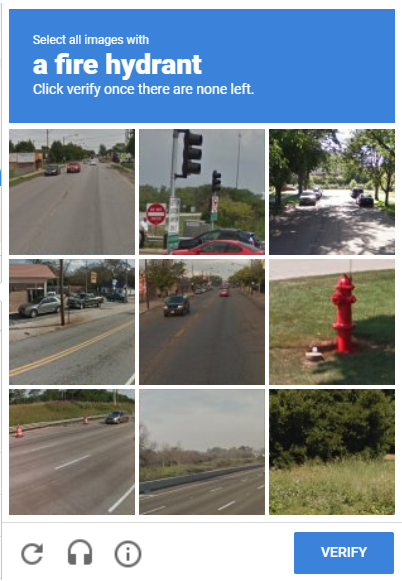
\includegraphics[width=0.4\textwidth]{images/captcha.png}
	\hspace{2em}
	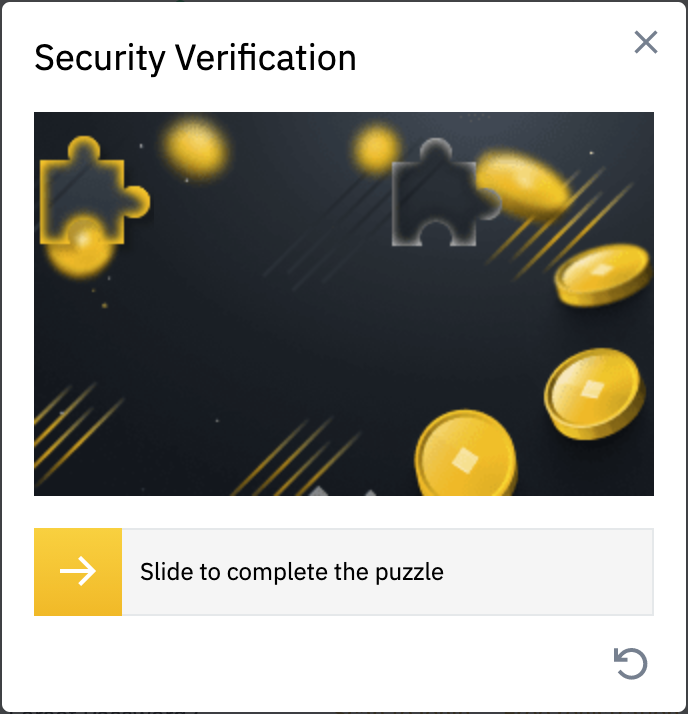
\includegraphics[width=0.4\textwidth]{images/captcha2.png}
	\caption{Mechanismus CAPTCHA používaný pro rozeznání lidského faktoru.}
	\label{img:captcha}
\end{figure}

\section{Hrozby na aplikační vrstvě}
Aplikační vrstva je nejcitlivější vrstva ze~tří důvodů: je nejblíže uživateli, úspěšný útok má největší dopad ze~všech dalších vrstev a~má největší škálu možných útoků. Všechny níže uvedené útoky by měly být odhaleny ochranami vyšších vrstev, tedy například aplikačním firewallem.

\subsection*{Phisning}
Cílem phishingu je získání citlivých dat ostatních uživatelů. Velmi častý způsob, jak lze tyto informace získat, je podvodný email nebo falešný účet na sociálních sítích. Tyto účty nebo emaily vypadají většinou velmi důvěryhodně a~vedou uživatele k~zadání citlivých dat (např.~jméno a~heslo do internetového bankovnictví), po jejichž vyplnění servírují citlivá data útočníkovi přesně podle jeho požadavků~\cite{bib:kyber_utoky}. Sociální sítě se snaží bránit těmto útokům, ale mnohdy je veškerá snaha neúspěšná. Phishing zpravidla probíhá automaticky, proto je vhodné tyto boty odhalit a~zakázat jim přístup na sociální síť.

\subsection*{Útoky DDoS na aplikační vrstvu}
Podobně jako klasické útoky DDoS (viz~\ref{sec:DDoS_force}) mají za cíl dostat webovou službu do stavu, kdy není schopna obsloužit normální uživatele. Oproti klasickému útoku DDoS však útočí na aplikační vrstvu, z~nich nejznámější je tzv.~HTTP floods attack (\uv{HTTP záplava}). To je útok, kdy se několik distribuovaných a~synchronizovaných stanic dotazuje HTTP dotazem GET nebo POST, ale server nestíhá odbavit takové množství požadavků a~donutí službu (či server) spadnout~\cite{bib:HTTP_flood}. Aplikační firewall by měl být schopen tento typ útoku odhalit.

\subsection*{SQL injection}
SQL injection útok může odhalovat mnoho citlivých informací uložených v~SQL databázi (např.~přihlašovací údaje, hesla, telefonní čísla atd.). SQL Injection se pokouší získat neoprávněný vstup do databáze vložením SQL kódu do formuláře. V~případě, že se útočníkovi podaří získat strukturu databáze, může jednoduše manipulovat s~daty uloženými v~databázi~\cite{bib:SQL_injection}. Data získaná pomocí formuláře by tedy měla být zkontrolována (např.~aplikačním firewallem), zda neobsahují škodlivý (spustitelný) kód a~předejít útokům tohoto typu.

\subsection*{Cross-Site Scripting}
Cross-Site Scripting (XSS) je typ útoku, kdy je škodlivý kód injektován na neškodný a~důvěryhodný web tak, že se útočník chová jako normální uživatel, avšak ukládá do webové databáze škodlivý skript. K~útoku dochází, když útočník získá kontrolu nad HTML obsahem, který je doručován uživateli webové aplikace, protože může do odesílané HTML stránky přidat vlastní JavaScriptový kód, který dříve uložil do databáze. Útočník může využít uživatelův účet k~získání citlivých informací, k~šíření spamu apod.~\cite{bib:XSS, bib:XSS_vut}. Ochrana webového serveru musí zabránit snaze nepovolených uživatelů o~jakoukoli manipulaci se soubory na serveru.

\subsection*{Broken Authentication and Session Management}
Příčinou tohoto útoku je chybná autentizace a~správa relace, protože může dojít k~odcizení uživatelských účtu. Obvyklá příčina je špatné schéma správy relací a~autentizace uživatelů (např.~nevhodný způsob obnovy hesla)~\cite{bib:XSS_vut}. Automatičtí roboti mohou tento nedostatek webových stránek využívat např.~k~získání přístupu do cizího účtu.

\subsection*{Sensitive Data Exposure} 
Veškerá citlivá data, která se ukládají do webové databáze, by měla být důkladně zašifrována. Pokud tomu tak není a~útočník ovládne databázi, získá přístup k~citlivým datům, která jsou v~databázi uložena. Tento útok může mít vážné dopady, protože dokáže získat citlivé údaje a~zneužít jich. Je tedy důležité udržovat data na serveru zašifrovaná a~přístup k nim jistit aplikačním firewallem~\cite{bib:sensitive_data_exposure}.

% \section{Proxy server}
% \label{sec:proxy_server}
% Proxy server je \textit{transparentní prostředník} ve spojení mezi klientem a~serverem, který má více funkcí. Mezi tyto funkce většinou patří firewall (na aplikační vrstvě), avšak hlídá celkový síťový provoz a~snaží se ho různými způsoby optimalizovat. Ke~klientovi se chová jako server, na nějž klient odesílá požadavky a~k serveru se chová jako klient, který žádá dotazy na server. Proxy server může filtrovat komunikaci či ji nějakým jiným způsobem odposlouchávat nebo filtrovat. Proxy server může také uchovávat data v~cache, ukládat cookies nebo vyváženě rozkládat provoz na webových serverech (webový server zpravidla neznamená pouze jeden stroj, ale více strojů s~jedním doménovým jménem, mezi které je nutno vyvažovat provoz). 

\section{Analýza provozu}
Aplikační firewall používá k~odhalení automatických botů zpravidla více technik. Techniky spadající pod analýzu provozu lze definovat tím, že nepracují s~HTML kódem požadované stránky, ale snaží se identifikovat hosta a~na základě jeho chování určit, zda se jedná o~podezřelý provoz či nikoliv. O~každému hostovi, který je většinou definován IP adresou, může aplikační firewall ukládat několik informací týkajících se jeho chování, na jejichž základě později rozpoznává automatický přístup. Metody pracující na základě analýzy provozu jsou popsány v~následujících odstavcích.

\subsection*{Kontrola hodnoty \texttt{User-Agent}}
Aplikační firewall velmi často pracuje s~hodnotami v~HTTP hlavičce. Jednodušší boti neposkytují hodnotu \texttt{User-Agent} (viz~\ref{sec:user_agent}) a~aplikační firewall je může na základě absence těchto informací zařadit do gray IP listu (viz~\ref{sec:ip_lists}) či rovnou zakázat provoz. Tedy uživatel, resp. bot, který neposkytuje tyto informace a~aplikační firewall to odhalí, zpravidla řeší úlohu CAPTCHA~\ref{sec:captcha} nebo jiný Turingův test\footnote{Turingovy testy ověřují, zda má systém navštěvující webovou stránku lidskou inteligenci nebo ne.} pro přístup do webové služby.

\subsection*{Analýza četnosti návštěv}
Analýza četnosti návštěv je \textit{střednědobá technika}\footnote{Střednědobá technika znamená, že její zavedení vyžaduje nějaký časový rámec, například 2~týdny.}, která slouží k~rozpoznávání automatického přístupu na základě analýzy časů přihlašování. Pokud se \textit{časové intervaly} mezi jednotlivými přihlášeními jednoho uživatele liší velmi málo či vůbec, lze z~toho usoudit, že uživatel je automatický bot. Podobně lze analyzovat \textit{denní časy} přihlašování uživatele~--~pokud se uživatel přihlašuje pouze ve stejné nebo velmi podobné denní časy, může jít o~automatický přístup.

Aby tato ochrana odhalovala pouze automatické boty a~neblokovala provoz normálním uživatelům, je nutné analyzovat časy uživatelských přihlašování \textit{po určitou dobu} (čím déle, tím lépe~--~proto střednědobá technika), než bude uživateli např.~odebrán účet. Může se totiž stát, že se i~normální uživatel bude přihlašovat ve~velmi podobné denní časy, ale jistě se někdy přihlásí dříve nebo později (normální uživatel se nedokáže přihlásit každý den v~naprosto stejný čas). 

\subsection*{Analýza doby strávené na webu}
\label{sec:time_analysis}
Doba strávená uživatelem na webu bývá odlišná od doby strávené na webu v~minulých návštěvách. Jestliže aplikační firewall zjistí, že se doba strávená na stránce pohybuje stále ve stejných intervalech, může se jednat o~podezřelou aktivitu a~vést k~zařazení IP adresy do gray IP listu. Kvalitní informace o~průměrném čase stráveném na webové stránce lze získat dlouhodobým sledováním a~jsou odlišné v~závislosti na poskytované webové službě.

\subsection*{Analýza chování}
Analýza chování je složitá disciplína, která vyplývá ze~strojového učení~\cite{bib:behaviorAnalysis}. Aplikační firewall zkoumá, zda je chování uživatele (nebo automatického bota) podezřelé nebo ne. Mezi podezřelou aktivitu se řadí např.~prodleva mezi jednotlivými stisky klávesnice, velmi častá návštěva jednoho konkrétního místa na webu, počet kliknutí na určitý objekt na stránce nebo stejná doba strávená na webu (viz~\ref{sec:time_analysis}). 

\subsection*{Honeypots/honeynets}
Velké firmy, jako je Amazon či CloudFare, používají k~zachycení botů sítě honeynets (překlad:  \textit{\uv{medové sítě}}) po celém světě, které poskytují aktualizované informace o~botech aplikačním firewallům ve svých sítích. Typická stránka, která slouží jako honeypot (překlad:  \textit{\uv{hrnec medu}}), je stránka obsahující velké množství zdánlivě užitečných informací, čímž se stává lákavější pro automatické boty, kteří tuto stránku navštíví za účelem získání velkého množství kvalitních dat. 

\section{Úprava HTML dokumentu}
Většina automatických botů, kteří se snaží o~získání dat z~webové stránky, má přesně danou pozici a~dokonale zná HTML (viz~\ref{sec:html}) strukturu navštívené stránky. Na základě této znalosti dokážou automatičtí boti získávat požadovaná data. Při změně této struktury (např.~hlubší zanoření HTML elementů) může dojít k neschopnosti automatického robota získat požadovaná data.

\subsection*{Změna identifikátorů HTML tagů}
Jedna z~možností, jak se bránit automatickému přístupu, je \textit{změnit identifikátory tagů v~HTML dokumentu}. Tato ochrana vychází z~předpokladu, že si bot stáhne webovou stránku a~poté z~ní extrahuje data, která se nacházejí na předem určených místech. Tato místa jsou označena unikátními jmény, díky nimž dokáže bot najít požadovaná data. V~případě, jsou tato jména změněna na náhodnou sekvenci písmen či čísel\footnote{Provozovatel má systém, který mu udržuje původní smysluplná jména značek, přičemž automaticky generuje HTML dokument s~náhodnými jmény značek a~který pravidelně aktualizuje na webovém serveru.}, bot nedokáže najít požadovaná data a~ztrácí zájem získávat data z~tohoto serveru. Tento způsob ochrany zpravidla nemá na normálního uživatele zásadní dopad.

Další způsob, jak udělat HTML dokument hůře čitelný pro automatického bota, je změna pozic jednotlivých částí (změnit design webové stránky), ve kterých se mohou vyskytovat potenciálně užitečná data. Znamená to, že každá stránka pravidelně mění svůj vzhled. Tento přístup má však jisté nevýhody, zejména jde o~uživatelské pohodlí. Každá změna, která se na vzhledu stránky projeví, může mít negativní dopad na uživatele a~může vést k~ztrátě jeho zájmu o~publikovaný obsah.

\subsection*{Website cloaking}
Website cloaking (přeloženo jako \textit{\uv{maskování webových stránek}}) je chování webových stránek, které se snaží doručovat jiný obsah webovým botům než běžným prohlížečům. Mezi cloaking patří např.~poskytnutí pouze čisté HTML stránky webovým robotům, ve které není zahrnuta žádná grafika. Tato technika bývá často používána pro internetové vyhledávače kvůli snazšímu vyhledání klíčových slov. Website cloaking může ale být použit jako obrana proti automatickému přístupu například tak, že data na této stránce budou upravena či nebudou na stránce obsaženy vůbec.

\subsection*{Informace v~obrázku}
Veškerý text, který je prezentován na webové stránce, lze převést na obrázek a~na stránce změnit text na odpovídající obrázky. Bot navštěvující stránku musí tedy pomocí OCR\footnote{Optical Character Recognition, více o~OCR lze najít na \href{https://en.wikipedia.org/wiki/Optical_character_recognition}{Wikipedii}.} rozpoznat uvedený text a~převést ho na textovou podobu. Tento způsob ochrany je poměrně účinný proti jednodušším botům, avšak pokročilejší boti zejména s~umělou inteligencí si s~obrázkem dokážou relativně snadno poradit. Velká nevýhoda textu v~obrázku je výrazně vyšší uživatelské nepohodlí, protože webový prohlížeč uživatele stahuje více dat (načítání stránky je pomalejší). Dalším problémem, který uživatel mnohdy pocítí, je nemožnost pracovat s~funkcemi jako je kopírování textu nebo hledání textu na stránce. To opět může vést k~odchodu a~nespokojenosti potenciálního klienta.

\bigskip

Z výše uvedeného je zřejmé, že neexistuje dokonalá ochrana a~je poměrně náročné bránit se automatickým botům. Nejlepší ochrana je tedy zkoušet nové způsoby a~kombinovat je s~těmi osvědčenými s~cílem, že uživatel nic nepozná zejména na rychlosti odezvy a~designu uživatelského rozhraní. 

\chapter{Způsoby automatického přístupu}
\label{chap:auto_approach_to_web}
Jak název napovídá, jde o~naprogramovaný automatický přístup na webové stránky, z~něhož má prospěch ve většině případů provozovatel bota, avšak v~některých případech může prosperovat i~provozovatel webového serveru. Bot je tedy program, který dle daných podmínek pracuje s~obsahem na webu ve snaze simulovat normálního uživatele. Jinými slovy, bota si lze představit jako člověka, který pracuje s~webovou stránkou (pracuje s~daty na dané stránce) podle určitých pravidel nebo naučených postupů. Pokud webový server chce umožnit přístup botům, tak poskytuje \textit{speciální rozhraní API}, přes něž mohou tyto automaty komunikovat. V~opačném případě je nutné stránky navštěvovat jiným způsobem~--~\textit{webscrapingem}.

Automatický přístup na web (tedy i~sociální sítě) lze tedy realizovat více způsoby. Některé metody jsou provozovány se~souhlasem provozovatele a~jejich použití je v~souladu se~zájmu dané stránky. Tento způsob se nazývá \textit{API} a~věnuje se mu kapitola~\ref{sec:api}, nicméně cílem této práce není popsat tuto metodu. Na druhé straně proti API existuje metoda, jak získávat data z~webových stránek bez použití API, nazývaná \textit{webscraping}. Websraping nabízí oproti API větší škálu využití a~proto bývá využíván pro účely, které mohou být nežádoucí pro danou sociální síť (provoz přes API lze kontrolovat a~popř.~zablokovat). Velká nevýhoda API je totiž omezené spektrum možností, které se s~API dají provádět~--~provozovatel sociální sítě nemá pochopitelně zájem o~to, aby se na jeho síti šířil SPAM či jiné podobné věci. Tato práce se zabývá zejména přístupem na webovou stránku pomocí webscrapingu.

\section{API}
\label{sec:api}
Application Programming Interface (API) je obecný název pro rozhraní programovatelných aplikací. Pomocí API se dokážeme připojit k~lokálnímu či vzdálenému programu nebo službě a~využívat jeho funkcí, získávat nebo ukládat data či s~ním jinak komunikovat podle předem daných pravidel. Na obrázku~\ref{img:api} je schéma komunikace API: klient se táže API serveru Bittrex na kryptoměnové trhy, které je možné obchodovat, a~server mu je ve formátu JSON posílá zpět. API se dělí podle jeho použití na několik druhů. Tím je například API operačních systémů pro komunikaci operačního systému a~služby běžící na dané stanici, JavaScript API atd.~\cite{bib:API_introduction}. 

\begin{figure}[hbt]
	\centering
	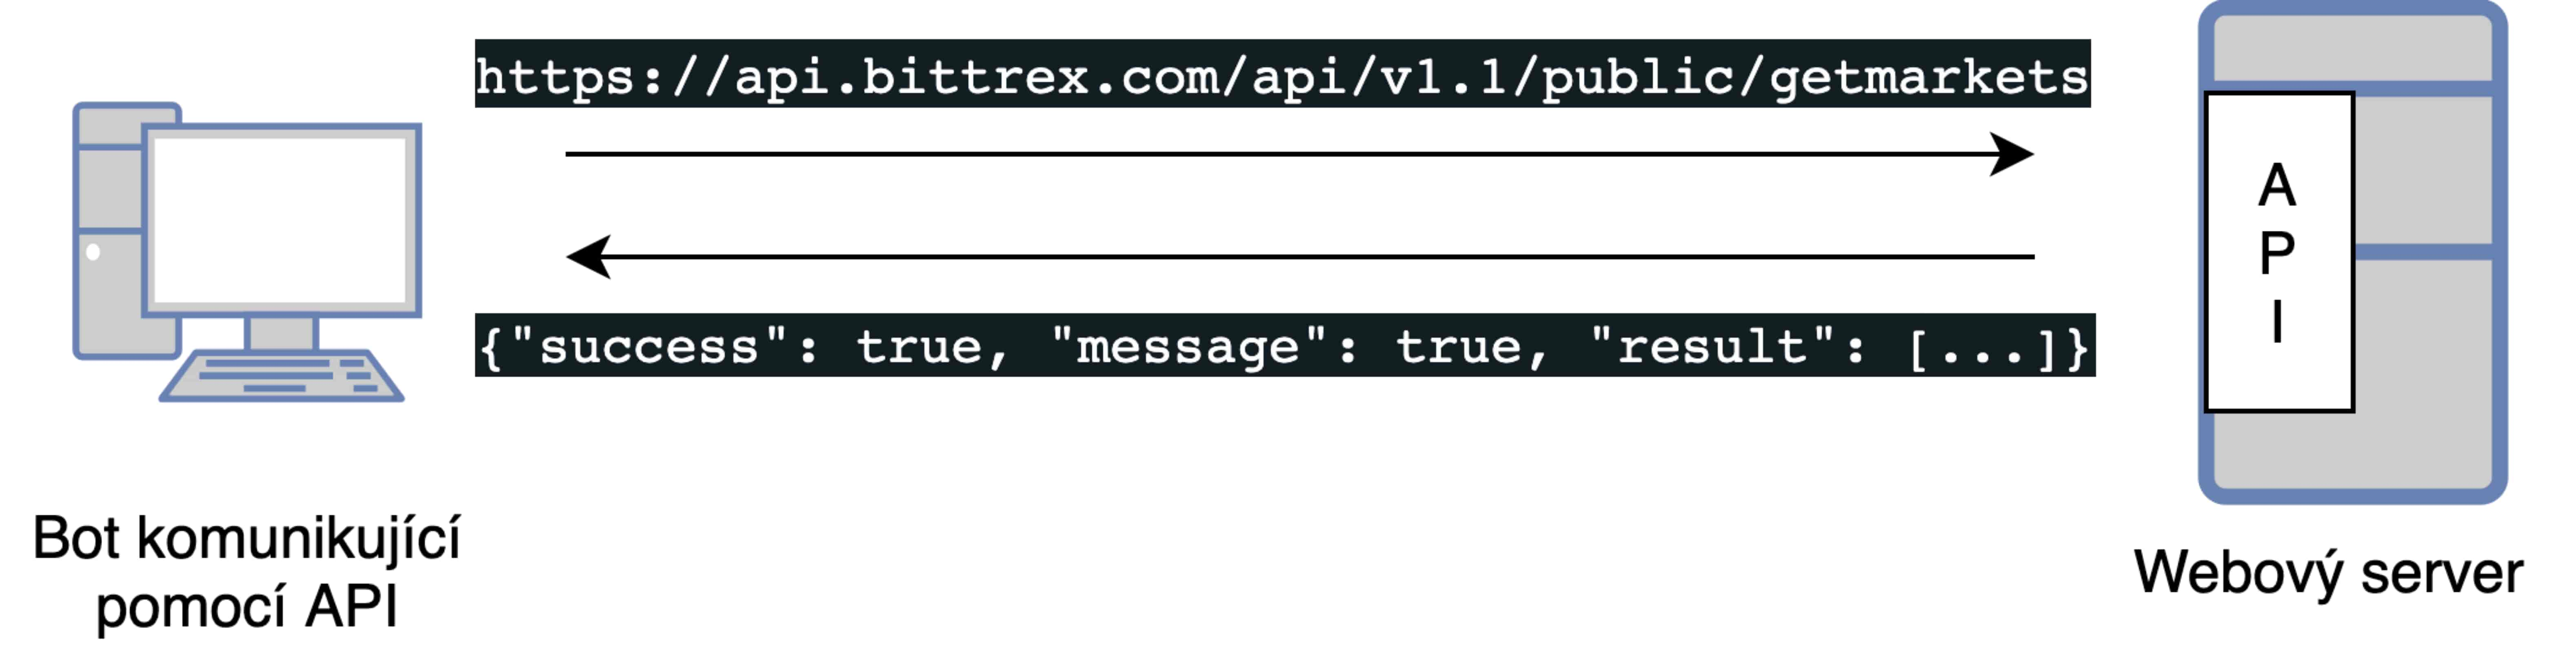
\includegraphics[width=0.8\textwidth]{images/API.jpg}
	\caption{Získávání dat pomocí API}
	\label{img:api}
\end{figure}

\subsection*{Third-party API}
Velké firmy, jako jsou Facebook, Google či PayPal, poskytují ostatním vývojářům jiných webových stránek svoje rozhraní API. To slouží k~využívání dat, která firma poskytující API vlastní. Uživatel využívá Thirt-party API například při vytváření účtu na webové stránce, kdy tato webová stránka požádá o~data o~uživateli Facebook, a~ten následně poskytne data (např.~jméno a~profilovou fotku) o~uživateli (pochopitelně se souhlasem daného uživatele)~\cite{bib:third_party_API}. To výrazně zjednoduší průběh vytváření nového účtu, protože uživatel vytvoří účet doslova jedním kliknutím. Další přihlašování probíhají také jednodušeji, protože se uživatel může přihlásit například pomocí účtu na Facebooku a~nemusí si pamatovat žádné další heslo.

\section{Webscraping}
\label{sec:webscraping}
Jde o~aktivitu, která se snaží dostat data z~webových stránek\footnote{Ačkoli se tato práce zabývá automatickým přístupem na sociální sítě, je v~této kapitole diskutováno obecně o~automatickém přístupu na webové stránky (sociální sítě jsou podmnožina webových stránek).} pomocí \textit{automatického programu}. Cílem webscrapingu je nahradit co nejdůvěryhodněji webový prohlížeč, simulovat uživatelskou interakci a~překonat ochranu proti automatickému přístupu (pokud nějaká existuje). Data, která jsou tímto způsobem získána, může sám webscrapingový program nebo jeho majitel dále upravovat či s~nimi nějak dále pracovat. Tento způsob získávání dat probíhá relativně často bez vědomí vlastníka webové stránky, ze~které jsou data dolována. Webové servery se snaží tomuto přístupu bránit, k~čemuž mají mnoho důvodů, nicméně je nutno dodat, že ochrany proti automatickému přístupu bývají neefektivní vůči vynaloženým nákladům. Pokud ochrana webového serveru odhalí automatický přístup, má několik možností, jak se zachovat~--~tyto možnosti jsou například:

\begin{itemize}
  \item \textbf{Nezasahovat}~--~nechat automatického bota pokračovat ve své činnosti.
  \item \textbf{Obfuskovat\footnote{\textit{Obfuskace} je proces, při kterém se upraví zdrojový kód tak, aby se stal (téměř) nečitelným, ale jeho funkčnost zůstane zachována. Používá se například jako ochrana vlastnictví autora~\cite{bib:obfuskace}.} obsah}~--~poskytnout automatickému botovi stránku s~upravenou strukturou \textit{zdrojového kódu} a~tím mu znesnadnit čtení obsahu.
  \item \textbf{Zakázat provoz}~--~zablokovat provoz z~IP adresy či webového prohlížeče nebo zablokovat uživatelský účet (pokud existuje).
\end{itemize}

Jedním z~důvodů, proč se bránit webscrapingu, je vytíženost serveru. Automatický server totiž může provádět takové operace, že se webová stránka stane pro ostatní uživatele obtížněji použitelná (např.~pomalejší odezva). Dalším důvodem, proč se bránit webscrapingu, je ochrana dat, která jsou na stránce obsažena. Některá data jsou sice veřejně dostupná, ale je nežádoucí, aby byla získávána automaticky. Struktura získávání dat webscrapingem je znázorněna na obrázku~\ref{img:webscraping}.

\begin{figure}[hbt]
	\centering
	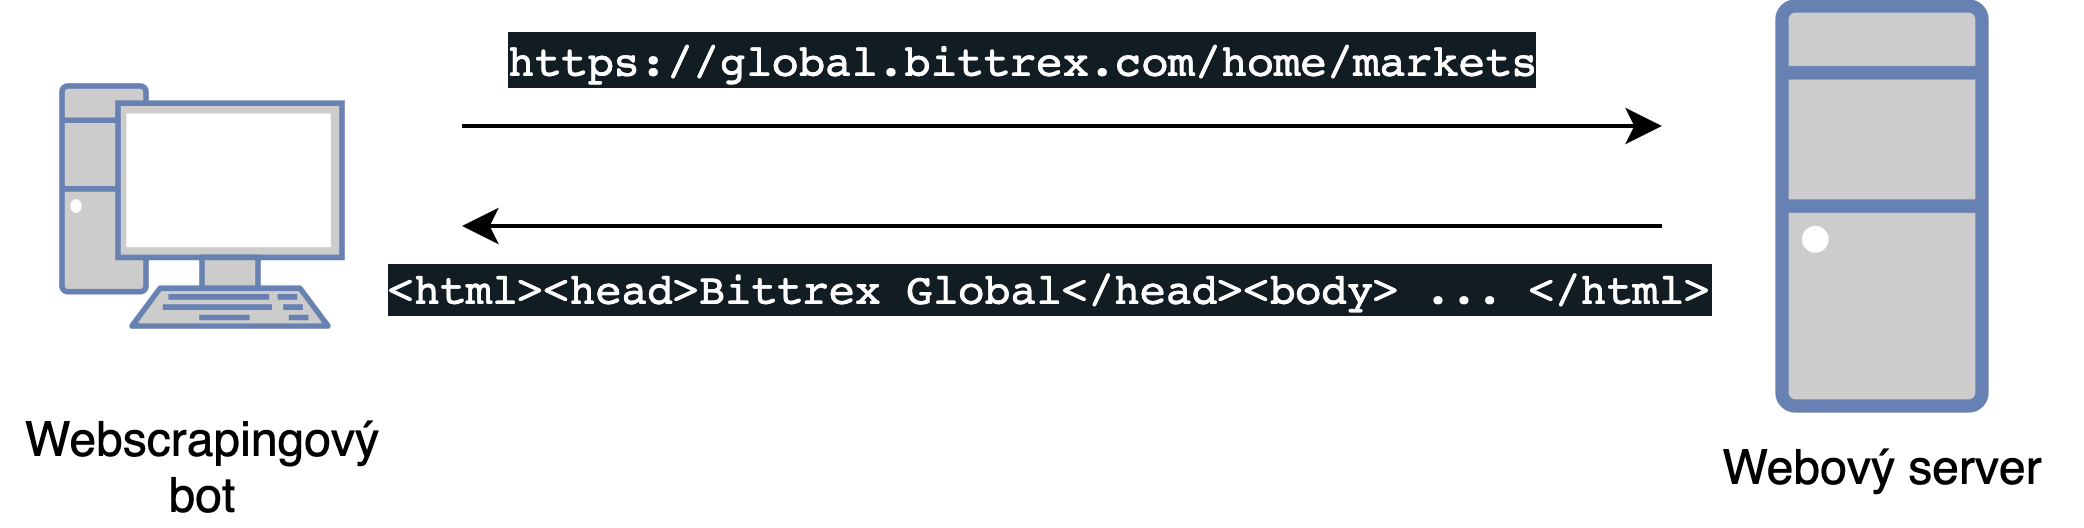
\includegraphics[width=0.8\textwidth]{images/webscraping.png}
	\caption{Průběh získání dat pomocí webscrapingu}
	\label{img:webscraping}
\end{figure}

\subsection*{Využití webscrapingu}
Když existují rozhraní API, přes která lze bez problémů a~se souhlasem druhé strany komunikovat, proč tedy existuje metoda webscraping? Po přehlédnutí poškození druhé strany a~jakýchkoli jiných druhů hackerského útoku, má velké využití v~situacích, kdy je zkrátka člověk samotný moc pomalý. Jde například o~situaci, kdy se očekává vydání lístků na koncert, o~které bude pravděpodobně obrovský zájem. Uživatel, který o~tyto lístky velmi stojí, využije webscrapingu (ačkoli je to poněkud nespravedlivé k~ostatním) a~bot mu tyto lístky nakoupí přesně podle jeho požadavků.

\subsection*{Webscraping na sociálních sítích}
Každá sociální síť si chce vytvořit či udržet dobrou pověst a~jejím hlavním cílem je, aby byl uživateli předkládán zajímavý obsah a~při trávení času na sociální síti se uživatel cítil pohodlně. V~případě sociálních sítí zpravidla není zásadní problém vytíženost serveru, kterou by automatický přístup mohl negativně ovlivnit. Hlavní důvod, proč se tyto sítě brání automatickému přístupu je, že by byl uživatelům servírován nezajímavý nebo podvodný obsah. Na to by uživatelé mohli reagovat odchodem ze~stránky, což by vedlo k~menšímu počtu zobrazení reklam. To by citelně snížilo zisk sociální sítě z~reklamy a~menší důvěru uživatelů v~tuto síť. Dalším důležitým důvodem je ochrana citlivých uživatelských dat nebo nastavení, jejichž soukromí může být narušeno. Z~tohoto důvodu se sociální sítě usilovně snaží zabránit automatickému přístupu na jejich stránky. Ochrana proti automatickému přístupu sociálních sítí by měla být z~výše uvedených důvodů pokročilá a~díky tomu je vhodné studovat aplikační firewally právě na sociálních sítích.

\section{Selenium}
\label{sec:selenium}
Selenium je sada nástrojů publikovaných ve formě otevřeného kódu (\textit{opensource}) sloužících pro automatizaci webových prohlížečů a~testování webových aplikací. Dokáže věrně simulovat webový prohlížeč Google Chrome (Selenium WebDriver, více~\ref{sec:selenium_webdriver}) a~kvůli tomu je často využíván právě pro účely webscrapingu. Selenium používá velké množství firem, mezi něž patří např.~MIT, Google, Fitbit a~další~\cite{bib:selenium_automatizace}. Sada nástrojů Selenium je napsána v~jazyce Java, čímž umožňuje použití na mnoha platformách. Tato sada nástrojů je velmi flexibilní z~hlediska použitého programovacího jazyka, protože podporuje jazyky jako Perl, Python, Ruby, Java, C\#, PHP a~další~\cite{bib:selenium_automatizace}.

Selenium je kompatibilní se všemi nejpoužívanějšími prohlížeči, čímž se stává atraktivnější pro testování webových aplikací. Je totiž důležité, aby tyto aplikace běžely správně na všech používaných webových prohlížečích. Sada nástrojů je open-source, je tedy zdarma pro všechny uživatele.

Selenium Suite se dělí na 4~projekty: \textit{Selenium IDE}, \textit{Selenium Remote Control}, \textit{Selenium WebDriver} a~\textit{Selenium Grid}~\cite{bib:selenium_projekty}. Schéma rozdělení Selenia je uvedena na obrázku~\ref{img:selenium}. Každý projekt z~této sady je vhodný pro něco jiného a~nabízí jiné možnosti využití pro testování webových prohlížečů nebo testování webových aplikací. 

\begin{figure}[hbt]
	\centering
	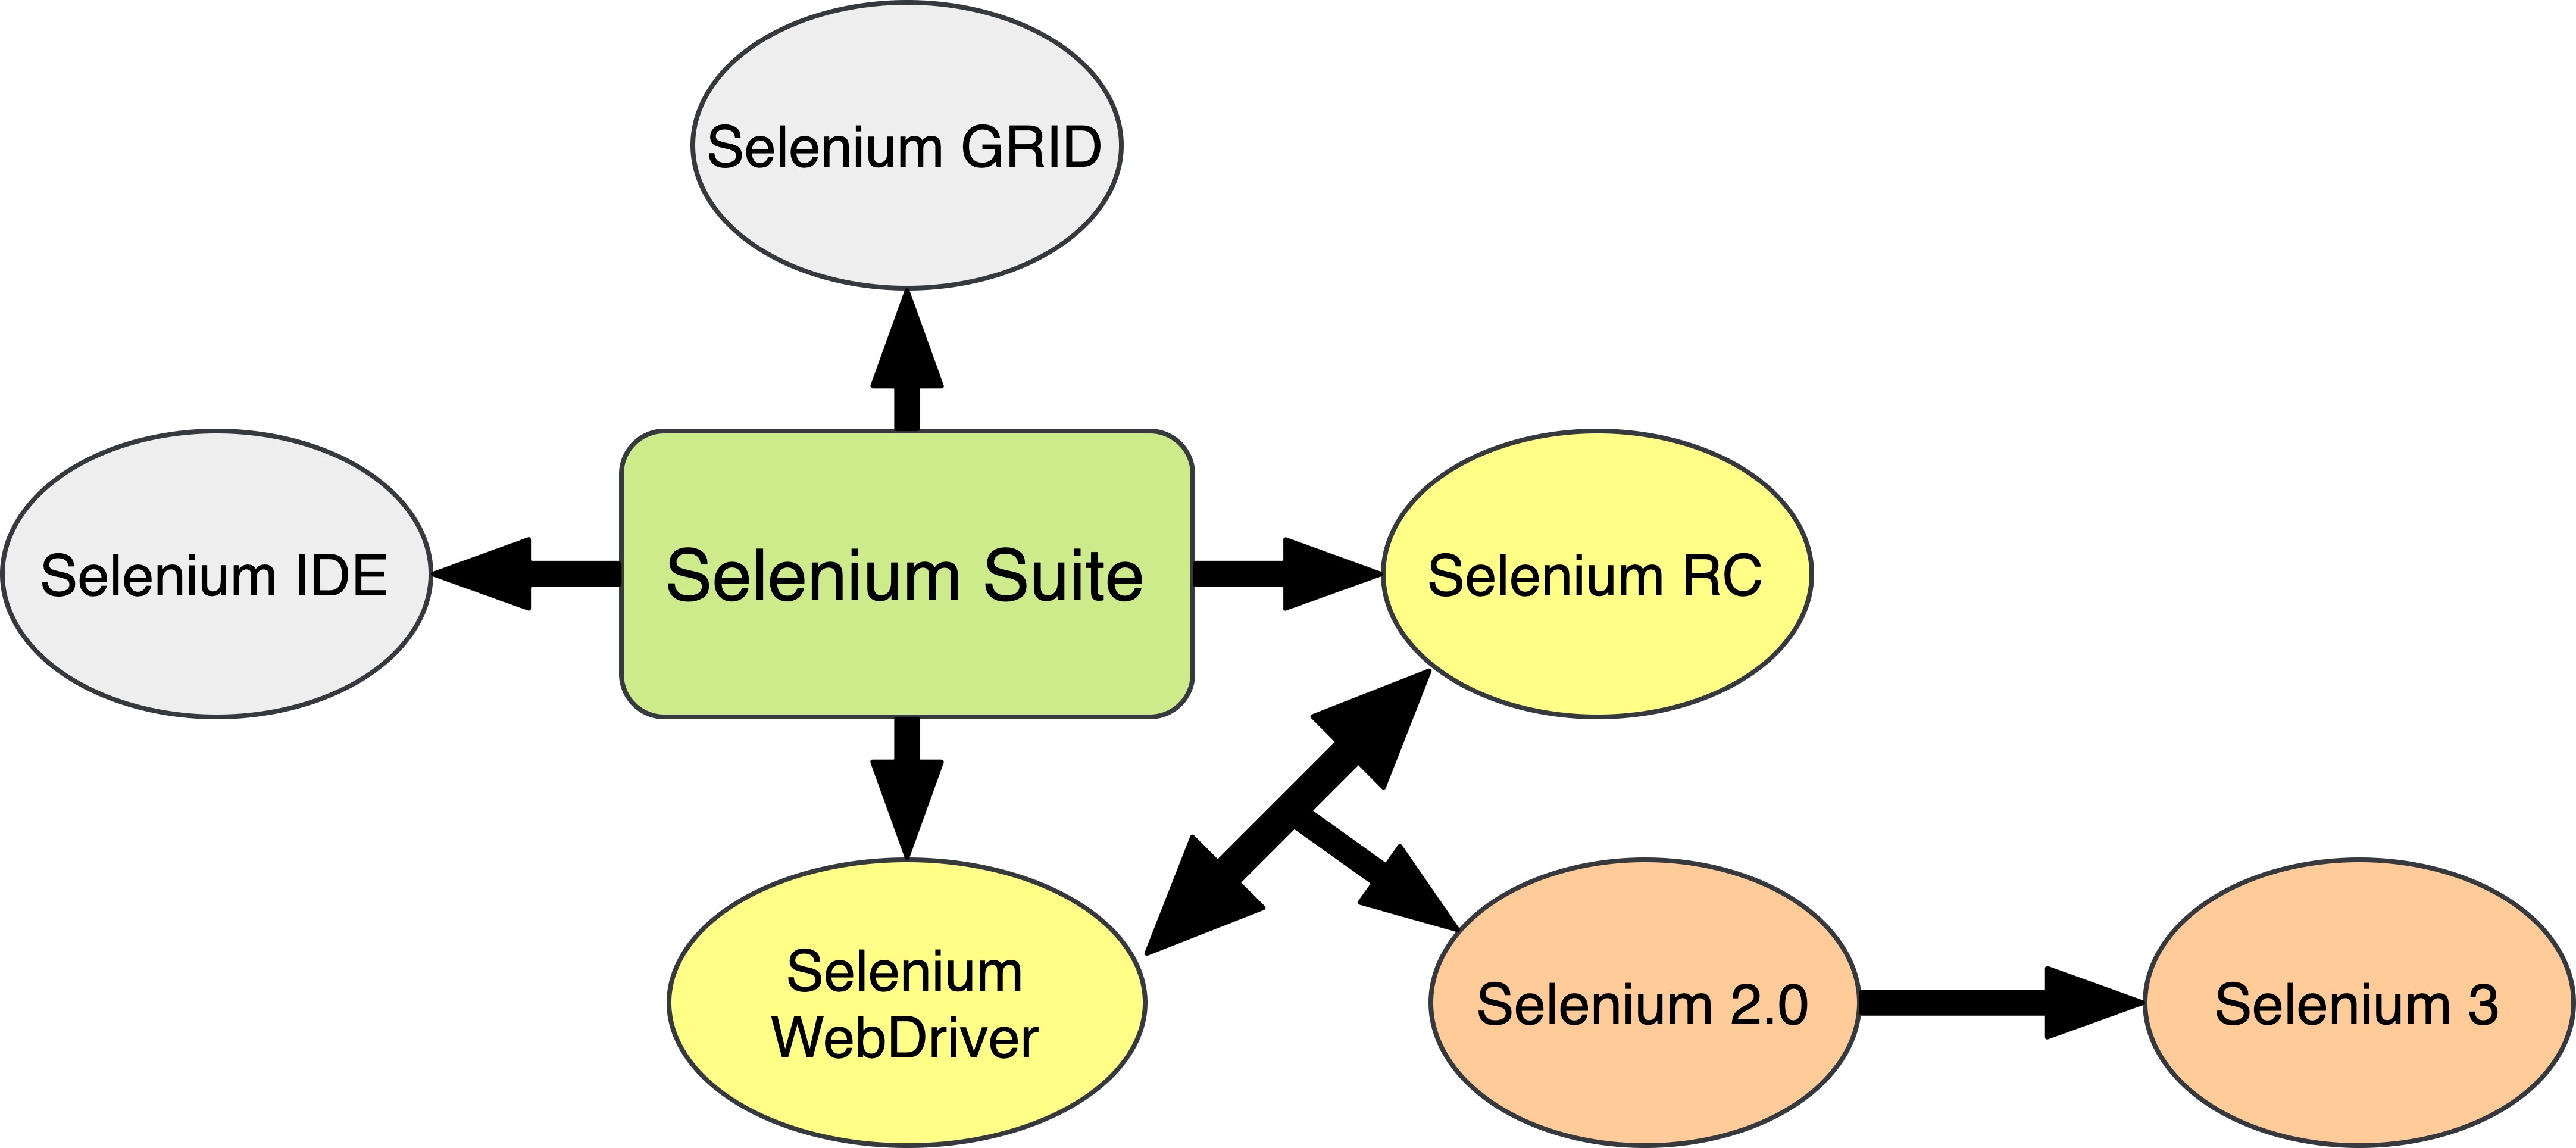
\includegraphics[width=0.6\textwidth]{images/selenium.png}
	\caption{Architektura Selenium včetně tvorby Selenium 2.0~spojením Selenium~RC a~Selenium WebDriver}
	\label{img:selenium}
\end{figure}

\subsection*{Selenium IDE}
Selenium IDE (\textit{Selenium Integrated Development Environment}) je doplněk do webového prohlížeče (dříve pouze Firefox, dnes už i~Google Chrome~\cite{bib:selenium_chrome}). Pomocí něj můžeme vytvářet automatické testy, které fungují na základě nahrávání interakcí uživatele s~webovou stránkou. Tento záznam lze pomocí Selenium~IDE zpětně přehrát. Instalace Selenium~IDE je velmi jednoduchá: v~prohlížeči Google Chrome (nebo v~prohlížečích pracujících s~jádrem Google Chrome) lze aplikaci nainstalovat přes Obchod Chrome; v~prohlížeči Firefox přes Firefox~Add-ons. 

Na obrázku~\ref{img:selenium_IDE} je ukázka aplikace Selenium IDE, která otevře hlavní stránku sociální sítě Twitter.

\begin{figure}[hbt]
	\centering
	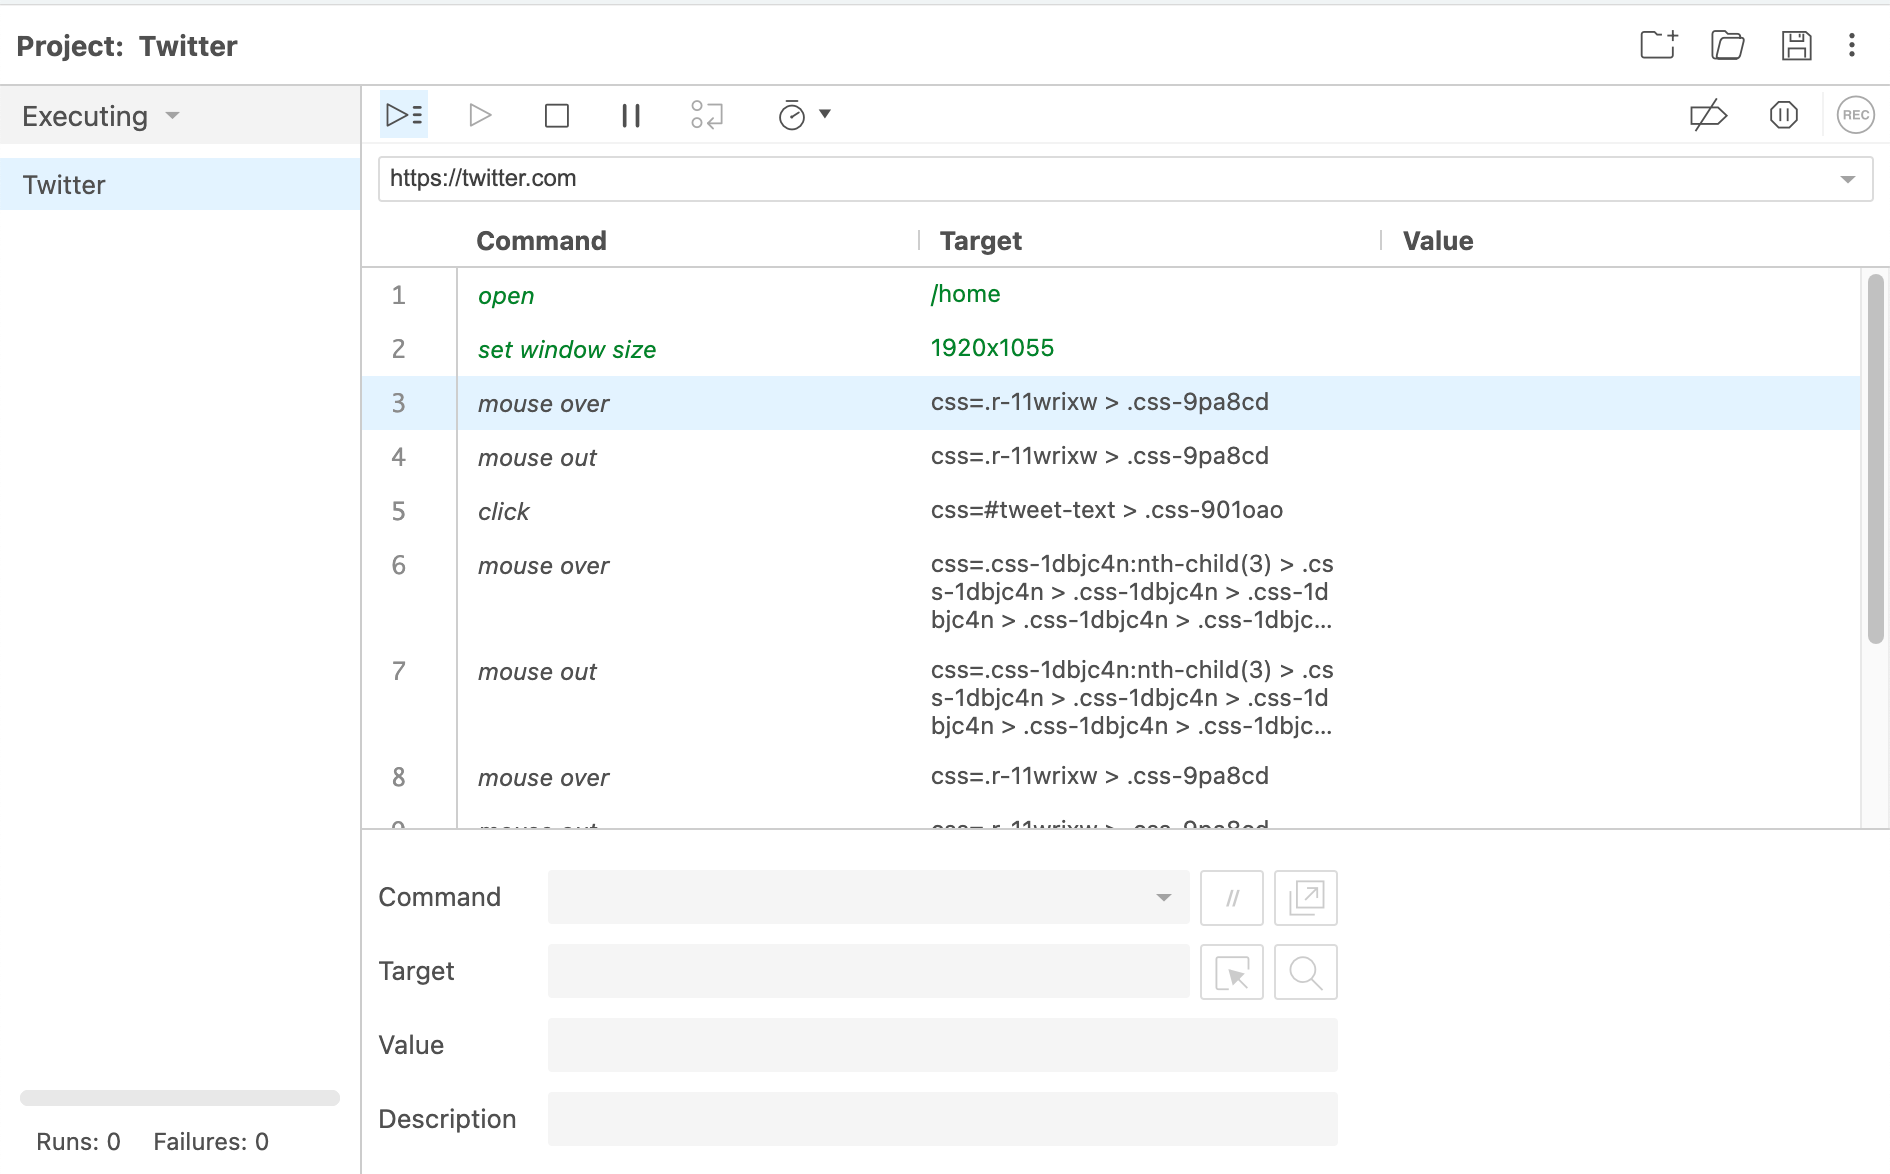
\includegraphics[width=0.6\textwidth]{images/selenium_IDE.png}
	\caption{Ukázka průběhu simulace přístupu na webovou stránku programem Selenium IDE}
	\label{img:selenium_IDE}
\end{figure}

\subsection*{Selenium Remote Control}
Selenium~RC je testovací nástroj klient-server. Umožňuje interpretovat automatické testy webových aplikací v~libovolném programovacím jazyce podporovaném Selenium Suite na jakékoli webové stránce nad protokolem HTTP(s) využívající JavaScript. Zahrnuje také HTTP Proxy server\footnote{Proxy server je neviditelný prostředník mezi klientem a~serverem a~může například filtrovat nebo optimalizovat provoz.}, který dává důvěru prohlížeči, že testovaná webová aplikace pochází z~domény poskytované proxy serverem. Nevýhodou Selenia~RC je, že musí existovat server, který přijímá HTTP(S) požadavky od klienta (tento server může běžet na stejném i~vzdáleném fyzickém zařízení)~\cite{bib:selenium_tool_suite, bib:selenium_grid}. Architektura Selenium~RC je zobrazena na obrázku~\ref{img:selenium_remote_control}.

\begin{figure}[hbt]
	\centering
	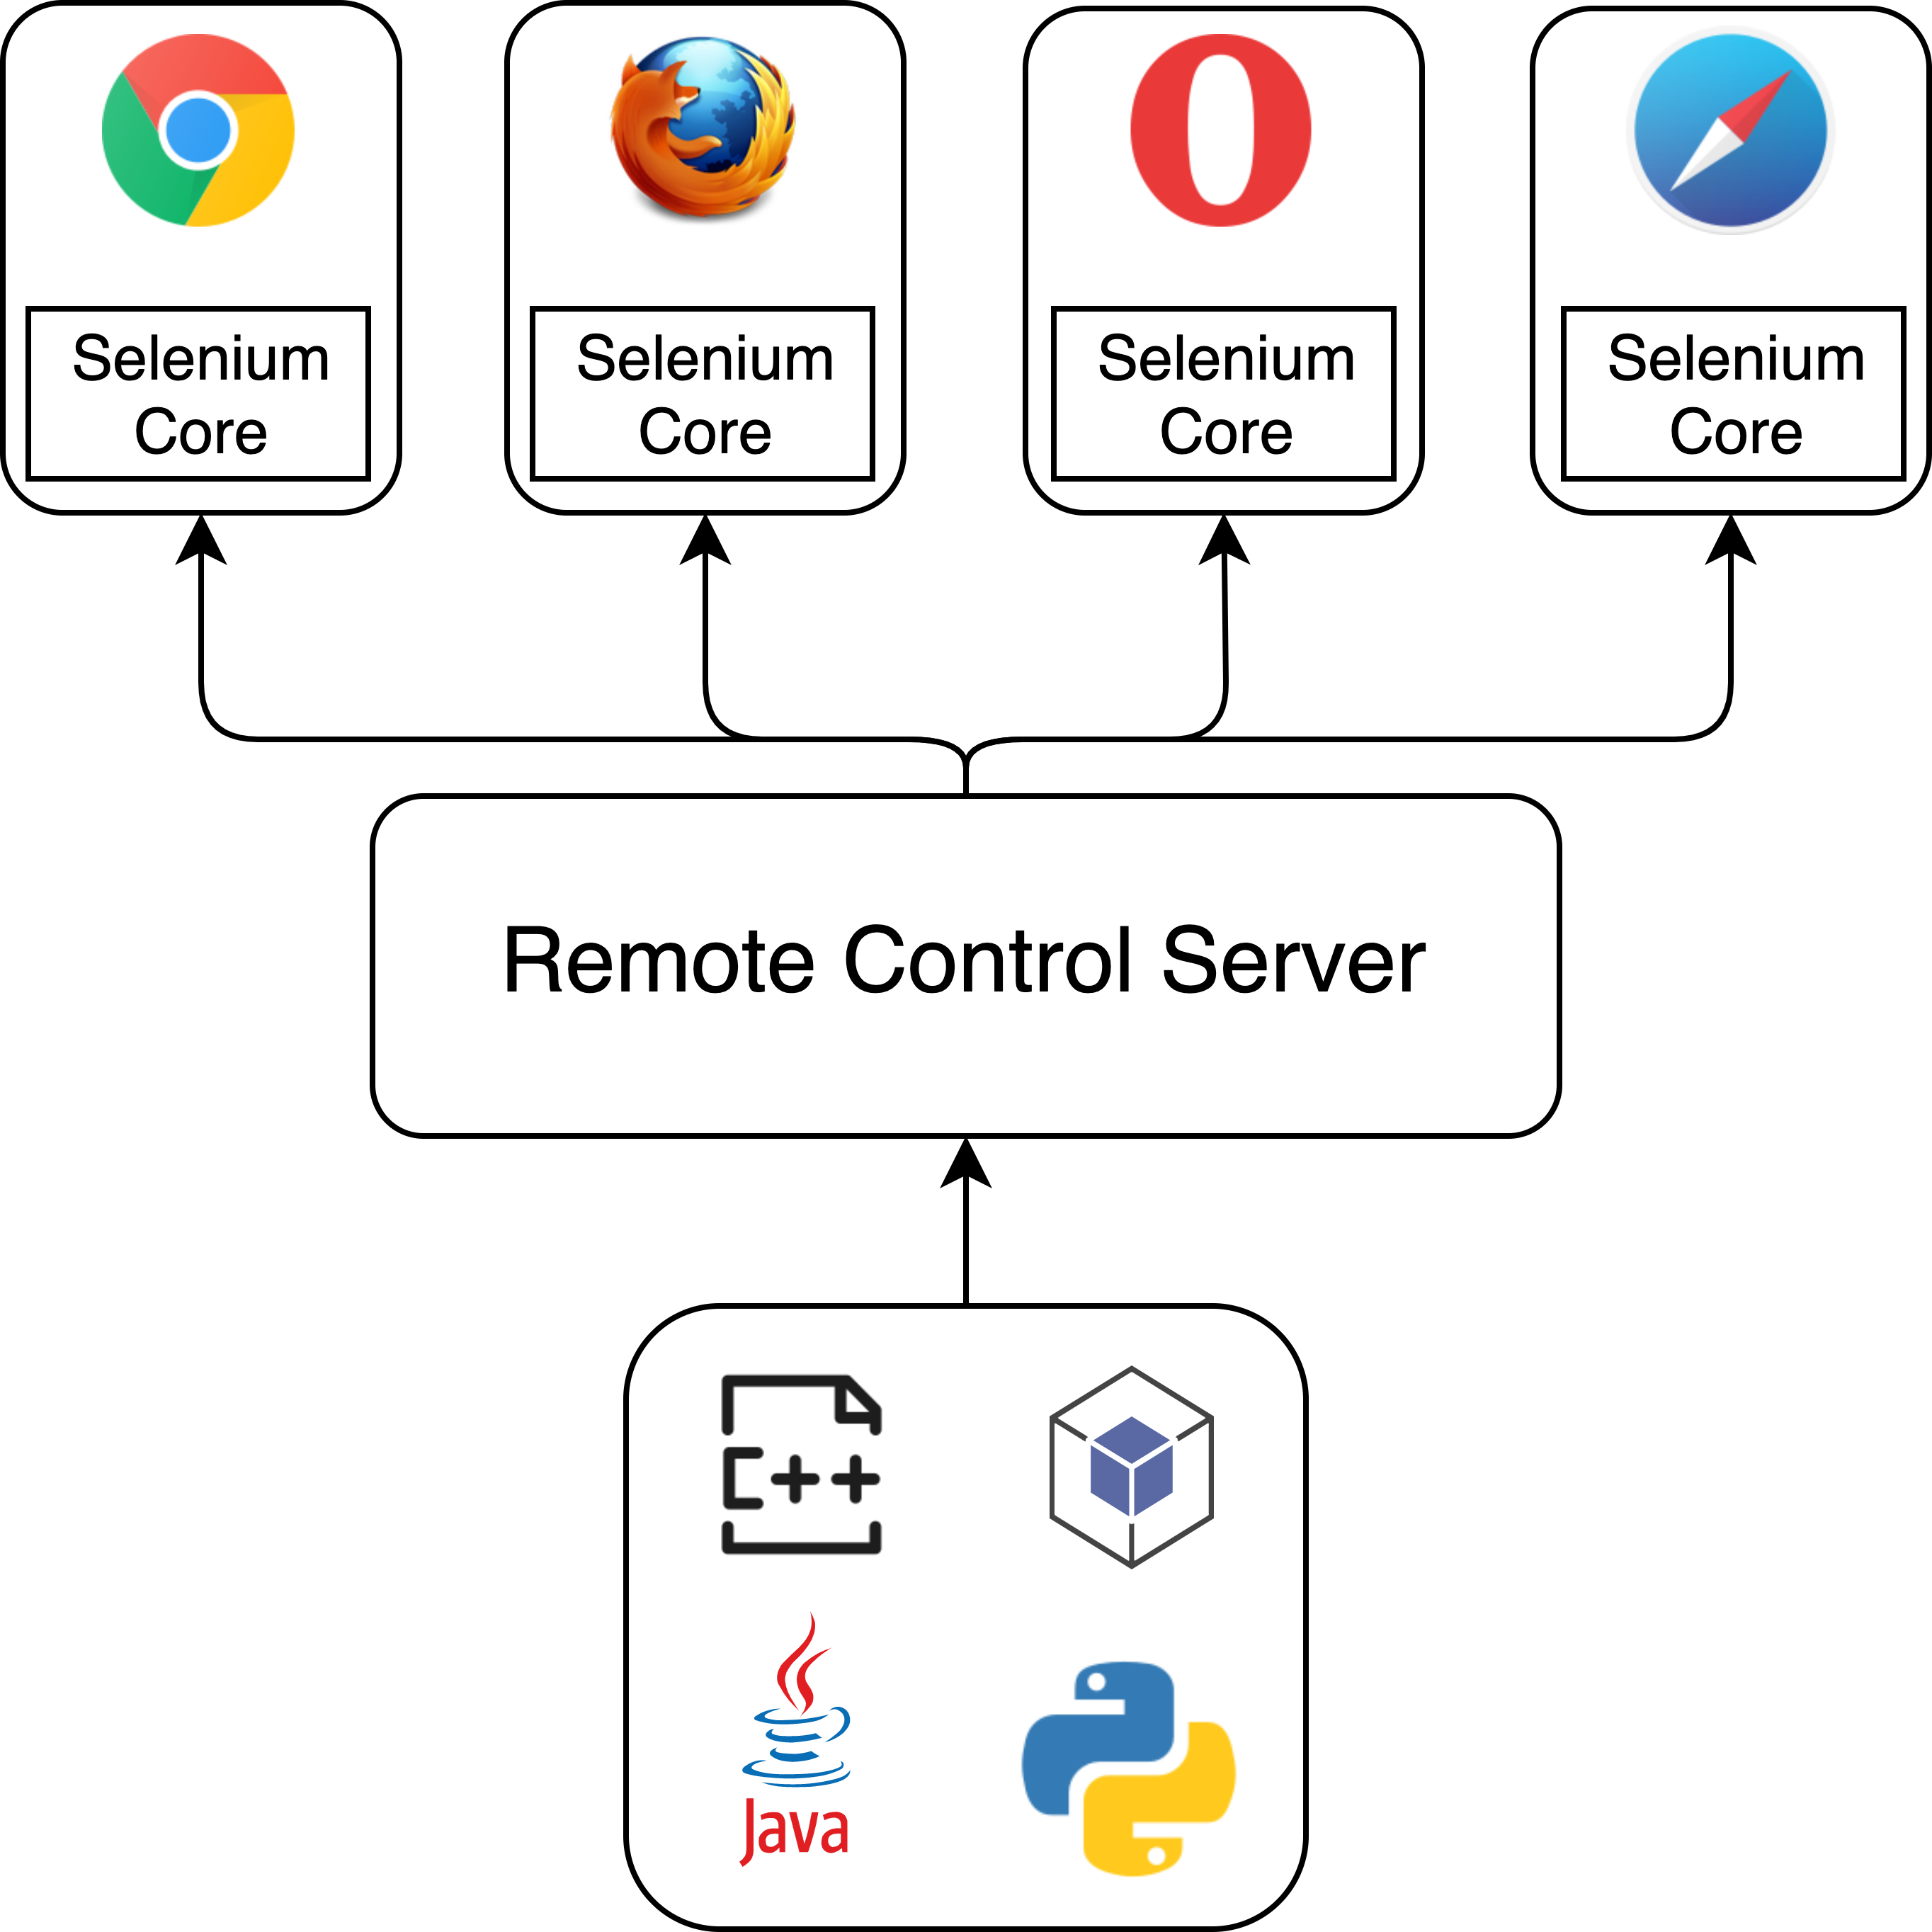
\includegraphics[width=0.6\textwidth]{images/selenium_remote_control.png}
	\caption{Selenium~RC architektura}
	\label{img:selenium_remote_control}
\end{figure}

\subsection*{Selenium WebDriver}
\label{sec:selenium_webdriver}
Selenium WebDriver je nástupce nástroje Selenium~RC a~zároveň nejdůležitějším nástrojem sady Selenium Suite. Oproti Seleniu~RC nabízí jednodušší a~stručnější programovací rozhraní, která řeší nedostatky a~omezení předchozí verze. Poskytuje programovací rozhraní pro vytváření a~provádění testovacích skriptů. Ty jsou psány za účelem identifikace jednotlivých prvků ve webové aplikaci a~dále jsou testovacími skripty vyhodnocovány akce, které testy provádí s~těmito prvky~\cite{bib:selenium_grid}. Cílem je větší podpora dynamických webových stránek, v~nichž se jednotlivé prvky často mění~\cite{bib:selenium_tool_suite}.

WebDriver funguje mnohem rychleji ve srovnání s~RC, protože WebDriver nepotřebuje spuštěný samostatný server, který provádí testy. Protože WebDriver přímo volá metody různých prohlížečů, je nutné, aby existoval pro každý prohlížeč samostatný ovladač (Mozilla Firefox Driver, Google Chrome Driver, Opera Driver apod.). V~aktuálně používané verzi Selenium 3~jsou nástroje WebDriver a~RC spojeny do jednoho nástroje WebDriver, do kterého je přidána další funkcionalita~\cite{bib:selenium_tool_suite}.

Na obrázku~\ref{img:selenium_webdriver} je znázorněna architektura nástroje Selenium WebDriver. Skládá se ze~tří komponent (zdroj~\cite{bib:selenium_webdrivers}): 
\begin{itemize}
  \item \textit{Selenium WebDriver} obsahující klientské knihovny pro vytváření a~provádění testovacích skriptů.
  \item \textit{Ovladače Selenium WebDrivers} specifické pro prohlížeč, které předávají požadavky z~WebDriveru.
  \item \textit{Prohlížeč Browsers}, který přijímá požadavky od ovladačů a~následně je zpracovává.
\end{itemize}

\begin{figure}[hbt]
	\centering
	\includegraphics[width=0.6\textwidth]{images/selenium_webdriver.jpg}
	\caption{Selenium WebDriver architektura}
	\label{img:selenium_webdriver}
\end{figure}

\subsection*{Selenium Grid}
Nástroj Selenium Grid je nástroj, který umožňuje provádění testů v~distribuovaném prostředí, tedy na různých strojích s~různými prohlížeči současně. Skládá se z~jednoho zařízení, která má roli \textit{Hub}~--~testovací server, a~libovolného počtu zařízení, která mají roli \textit{Node}~--~testovací uzel~\cite{bib:selenium_grid}. Výsledkem testování je tedy zkouška webové aplikace na různých počítačích s~různými prohlížeči a~odlišnými operačními systémy, čimž se výrazně urychluje doba testování webové aplikace.

Selenium Grid není příliš odlišný od ostatních nástrojů v~sadě Selenium. Je to velmi podobný nástroj jako Selenium WebDrive rozšířený o~možnost testovat aplikace paralelně v~odlišných prostředích.

\chapter{Testování aplikačních firewallů sociálních sítí}
\label{chap:app_firewalls_tests}
Sociální sítě mají pravděpodobně implementovány jedny z~nejpokročilejších ochran proti automatickým botům, a~proto je vhodné jejich studium. Sociální sítě totiž nemají z~jistých důvodů uvedených v~předchozích kapitolách zájem o~přístup automatických botů, nicméně na druhou stranu jsou právě sociální sítě jejich častým cílem a~sociální sítě se jim musí bránit. Znalost principu těchto aplikačních firewallů může být užitečnou inspirací pro~návrh nebo vylepšení ochran vlastních webových stránek či jiných veřejných služeb, které mohou být obětí automatických botů.

Kapitola začíná ukázkou chování skutečných uživatelů na sociálních sítích a~dále popisuje výsledky testování aktuálně používaných ochran proti automatickému přístupu. Poté popisuje možnosti přístupu na sociální sítě přes aplikační rozhraní API a~jeho srovnání s~webscrapingem. Testované sociální sítě jsou:

\begin{itemize}
  \item Facebook (včetně verze mBasic)
  \item Twitter
  \item LinkedIn
  \item YouTube
\end{itemize}

\section{Skutečné chování uživatelů na sociálních sítích}
Každý uživatel navštěvující určitou sociální síť má obvykle ve zvyku provádět jednotlivé akce postupně ve stejném pořadí. V~případech, kdy uživatel navštíví sociální síť kvůli nějakému účelu, např.~poslání zprávy či vyhledání informace\footnote{Mnoho uživatelů totiž navštěvuje sociální síť bezúčelně např.~kvůli závislosti.}, většinou svou posloupnost prvních akcí obejde. Testy popsané v~tabulkách č.~\ref{tab:soc_behaviour_P1},~\ref{tab:soc_behaviour_P2} a~\ref{tab:soc_behaviour_P3} popisují sekvence typického chování na sociálních sítích 3~osob. Tyto testy byly prováděny kvůli implementaci opatření navrhovaném v~této práci spočívající v~totožném chování po každém přihlášení. Testování chování osoby je prováděno pouze na platformách a~sociálních sítích, které daná osoba pravidelně navštěvuje. Většina časů v~tabulce je uvedena v~\textit{sekundách} a~časy jsou \textit{přibližné} (někdy může daná akce trvat kratší dobu, někdy delší dobu). Časy znamenají dobu uplynulou od spuštění sociální sítě, nikoli od poslední akce.

\definecolor{gray}{cmyk}{0,0.0,0.0,0.26}
\begin{table}[htbp]
  \begin{tabularx}{\linewidth}{
    |>{\centering\arraybackslash\hsize=0.5\hsize}X|% Socialni sit a~platforma
    >{\raggedright\arraybackslash\hsize=1.6\hsize}X|% Prvni akce
    >{\centering\arraybackslash\hsize=0.5\hsize}X|% Cas 1
    >{\raggedright\arraybackslash\hsize=1.6\hsize}X|% Druha akce
    >{\centering\arraybackslash\hsize=0.5\hsize}X|% Cas 2
    >{\raggedright\arraybackslash\hsize=1.3\hsize}X|% Poznamka
  }
\hline  
\rowcolor{gray}
\multicolumn{6}{|c|}{\textbf{Osoba 1}} \\ 

\hline \rowcolor{gray}
\multicolumn{1}{|c|}{\textbf{Platforma}} & \multicolumn{1}{c|}{\textbf{1. akce}} & \multicolumn{1}{c|}{\textbf{$\sim$~čas}} & \multicolumn{1}{c|}{\textbf{2. akce}} & \multicolumn{1}{c|}{\textbf{$\sim$~čas}} & \multicolumn{1}{c|}{\textbf{Poznámka}} \\
\hline
\textit{Facebook} mobil & Prohlédne si první 3~příspěvky & 15~s & Přečte si upozornění (pokud nějaká jsou) & 25~s & \\
\hline
\textit{Facebook} desktop & Zkontroluje upozornění a~přečte si ho & 8~s & Kontrola zpráv a~odepsání svým přátelům  & 35~s & Facebook na desktopu téměř nenavštěvuje \\
\hline
\textit{YouTube} mobil & Zkontroluje upozornění & 7~s & Podívá se na nějaké video podle upozornění & 75~s & \\
\hline
\textit{YouTube} desktop & Začne vyhledávat video s~požadovaným obsahem & 12~s & Prohlíží nalezená videa & 20~s & Na desktopu chodí vyhledávat videa pouze pokud potřebuje najít určitý obsah \\
\hline
\textit{Instagram} mobil & Prohlédne si přibližně 10~prvních stories & 50~s & Přečte si zprávy, popř.~na ně odepíše & 70~s & \\
\hline

\end{tabularx}

\caption{Typické chování na sociální síti první testované osoby}
\label{tab:soc_behaviour_P1}
\end{table}

\begin{table}[htbp]
  \begin{tabularx}{\linewidth}{
    |>{\centering\arraybackslash\hsize=0.5\hsize}X|% Socialni sit a~platforma
    >{\raggedright\arraybackslash\hsize=1.6\hsize}X|% Prvni akce
    >{\centering\arraybackslash\hsize=0.5\hsize}X|% Cas 1
    >{\raggedright\arraybackslash\hsize=1.6\hsize}X|% Druha akce
    >{\centering\arraybackslash\hsize=0.5\hsize}X|% Cas 2
    >{\raggedright\arraybackslash\hsize=1.3\hsize}X|% Poznamka
  }

\hline \rowcolor{gray}
\multicolumn{6}{|c|}{\textbf{Osoba 2}} \\ 

\hline \rowcolor{gray}
\multicolumn{1}{|c}{\textbf{Platforma}} & \multicolumn{1}{|c}{\textbf{1. akce}} & \multicolumn{1}{|c}{\textbf{$\sim$~čas}} & \multicolumn{1}{|c}{\textbf{2. akce}} & \multicolumn{1}{|c}{\textbf{$\sim$~čas}} & \multicolumn{1}{|c|}{\textbf{Poznámka}} \\
\hline
\textit{Facebook} mobil & Najde příspěvek, který zaujme & 18~s & Zareaguje na tento příspěvek a~přečte si komentáře & 30~s & Reklamy přeskakuje \\
\hline
\textit{YouTube} mobil & Podívá se na doporučená videa & 7~s & Video, které zaujme, si uloží do seznamu "Později" & 15~s & Videa neoznačuje \textit{To se mi líbí} ani nezanechává komentář \\
\hline

\end{tabularx}

\caption{Typické chování na sociální síti druhé testované osoby}
\label{tab:soc_behaviour_P2}
\end{table}

\begin{table}[htbp]
  \begin{tabularx}{\linewidth}{
    |>{\centering\arraybackslash\hsize=0.5\hsize}X|% Socialni sit a~platforma
    >{\raggedright\arraybackslash\hsize=1.6\hsize}X|% Prvni akce
    >{\centering\arraybackslash\hsize=0.5\hsize}X|% Cas 1
    >{\raggedright\arraybackslash\hsize=1.6\hsize}X|% Druha akce
    >{\centering\arraybackslash\hsize=0.5\hsize}X|% Cas 2
    >{\raggedright\arraybackslash\hsize=1.3\hsize}X|% Poznamka
  }

\hline
\rowcolor{gray}
\multicolumn{6}{|c|}{\textbf{Osoba 3}} \\ 

\hline  \rowcolor{gray}
\multicolumn{1}{|c|}{\textbf{Platforma}} & \multicolumn{1}{c|}{\textbf{1. akce}} & \multicolumn{1}{c|}{\textbf{$\sim$~čas}} & \multicolumn{1}{c|}{\textbf{2. akce}} & \multicolumn{1}{c|}{\textbf{$\sim$~čas}} & \multicolumn{1}{c|}{\textbf{Poznámka}} \\
\hline
\textit{Facebook} mobil & Najde příspěvek, který zaujme & 15~s & Zareaguje na tento příspěvek a~přečte si komentáře & 30~s & Reklamy přeskakuje \\
\hline
\textit{Facebook} desktop & Přečte si upozornění & 10~s & Prohlédne si prvních cca 7~příspěvků & 25~s & Zareaguje (nikoli okomentuje) příspěvek, který ho zaujme \\
\hline 
\textit{YouTube} mobil & Zkontroluje upozornění & 7~s & Podívá se na nějaké video podle upozornění & 120~s & \\
\hline
\textit{YouTube} desktop & Doporučená videa (2-3), která zaujmou, otevře v~nové záložce & 13~s & Postupně shlédne tato videa & 600~s & U~doporučených videí velmi často reaguje \textit{To se mi líbí} \\
\hline
\textit{Twitter} desktop & Prohlíží zeď, dokud nenarazí na sekci "Koho sledovat" & 18~s & Začne sledovat uživatele, jejichž obsah je přínosný & 17~s & Nečte upozornění \\
\hline

\end{tabularx}

\caption{Typické chování na sociální síti třetí testované osoby}
\label{tab:soc_behaviour_P3}
\end{table}

\section{Popis testování sociálních sítí}
Každá vybraná sociální síť byla otestována 5 testy. První dva jsou \textit{automatické}, třetí je \textit{poloautomatický} a~zbývající 2 jsou prováděny \textit{manuálně}. Automatické testy byly provedeny nástrojem Selenium WebDriver (viz~\ref{sec:selenium_webdriver}) s~využitím programovacího jazyka Python. Ostatní testy byly provedeny pomocí nástrojů uvedených v~seznamu níže. Každá sociální síť byla otestována v~tomto pořadí: 
\begin{itemize}
  \item \textit{Automatický test stejného chování} (automaticky pomocí Selenium WebDriver)
  \item \textit{Automatický test hromadného přístupu} (automaticky pomocí Selenium WebDriver)
  \item \textit{Test ověřování} \texttt{User-Agent} \textit{hodnoty} (manuálně pomocí Selenium WebDriver)
  \item \textit{Přístup z~prohlížeče Tor} (manuálně pomocí prohlížeče Tor)
  \item \textit{Test kódování identifikátorů HTML} elementů (manuálně pomocí prohlížeče Google Chrome)
\end{itemize}

\noindent
Výsledky testů jsou uvedeny v~jednotlivých sekcích zvlášť pro každou testovanou sociální síť. V~tabulkách je navíc uvedeno, zda sociální síť testuje lidskou inteligenci pomocí CAPTCHA (viz~\ref{sec:captcha}), protože se jedná o~jednoduchý a~efektivní způsob, jak zabránit vstup automatickým botům.

\subsection*{Automatický test stejného chování}
\label{sec:repeated_behaviour}
První automatický test zjišťuje, zda aplikační firewally sociálních sítí kontrolují podezřele velký počet přihlášení se do jednoho uživatelského účtu za krátký časový rámec. Dále odhaluje, zda aplikační firewally zkoumají uživatelské chování či nikoli. Jinými slovy test ověřuje, zda sociální sítě odhalují více přihlášení za sebou, po kterém se uživatel chová identicky. Aktivita, která proběhne vícekrát za sebou a~dělá naprosto samou věc, se totiž jeví jako podezřelá.

Selenium WebDriver po spuštění otevřel nové okno prohlížeče Google Chrome a~načetl přihlašovací stránku dané sociální sítě. Vyplnil uživatelské jméno a~heslo a~přihlásil se do sociální sítě. Na hlavní stránce se posunul o~1000~pixelů dolů, chvíli setrval a~vrátil se nahoru~--~tento pohyb na stránce se prováděl pouze kvůli větší důvěryhodnosti přístupu. Test kliknul na tlačítko \textit{To se mi líbí} u~prvního příspěvku a~5~sekund poté zavřel prohlížeč. Po zavření okna prohlížeče vyčkal test 30~sekund a~celý test opakoval znovu. Celý popsaný cyklus proběhl celkem $50\times$.

\subsection*{Automatický test hromadného přístupu}
\label{sec:dos_test}
Druhý test zkoušel (opět s~použitím Selenium WebDriver), stejně jako první test, přihlášení a~kliknutí u~prvního příspěvku na \textit{To se mi líbí}, nicméně tyto testy nebyly spouštěny postupně, ale v~jeden čas. Byl tedy spuštěn skript, který spustil 10\footnote{Více testů najednou nebylo možné spustit z~důvodu výkonu testovací stanice.} testů najednou, tedy podobný průběh jako při DoS útoku (viz~\ref{sec:DoS_force}). Účel analýzy byl ověřit, zda sociální sítě dokáží tuto aktivitu odhalit, popř.~jak se jí brání.

\subsection*{Test ověřování \texttt{User-Agent} hodnoty}
Tento test ověřoval, zda sociální sítě kontrolují správnost hodnoty \texttt{User-Agent}. Využívá skriptu z~prvního testu, ale je změněna HTML hlavička a~prohlížeč je spuštěn pouze jednou, nikoli $50\times$. Cíl testu byl stejný jako v~předchozích dvou testech, tedy kliknout na \textit{To se mi líbí}, ale žádost měla upravené hodnotu v~HTTP hlavičcce \texttt{User-Agent} na hodnotu \texttt{False\_user\_agent}. Příklad korektní hodnoty je popsán v~části~\ref{sec:user_agent}. Ačkoli se jedná o~poměrně jednoduchý test opatření, které lze jednoduše obejít, tak dokáže odfiltrovat alespoň triviální pokusy o~automatický přístup.

\subsection*{Přístup z~prohlížeče Tor}
Anonymizační systém Tor a~prohlížeč Torbrowser je popsán v~sekci~\ref{sec:tor_browser}. Jde tedy o~test přístupu z~různých IP adres, které jsou v~mnoha případech zařazeny do \textit{Black listů} nebo \textit{Gray listů} a~aplikační firewall tím dokáže jednoduše odhalit podezřelou aktivitu. Každou IP adresu lze alespoň přibližně lokalizovat, tedy pokud se jeden uživatel přihlašuje na sociální síť z~různých oblastí během krátkého času, aplikační firewall přístup zpravidla vždy zablokuje. Princip analýzy přístupu pomocí prohlížeče Tor spočívá jen v~přihlášení se na sociální síť.

\subsection*{Test kódování identifikátorů HTML elementů}
Každá načítaná stránka ve webovém prohlížeči se načítá pomocí HTML (viz~\ref{sec:html}). Webscrapingové automaty často pracují právě s~HTML strukturou a~jednotlivé elementy poznávají podle jedinečných HTML identifikátorů k~získání dat, které tento HTML element obsahuje. V~testu se ověřuje, zda webová stránka používá \textit{intuitivní} názvy HTML identifikátorů (např.~\texttt{heading}) nebo zda používá nějaké \textit{kódování} (např.~\texttt{0h4jek3iS}). Získání informací o~tom, zda sociální síť používá nějaké kódování HTML identifikátorů, bylo provedeno ručně pomocí nástroje Google Developers (více zde~\ref{sec:chrome_devtools}).

\section{Facebook}
Nejpopulárnější sociální síť Facebook\footnote{\href{https://www.facebook.com}{https://www.facebook.com}} je platforma, která byla původně plánovaná jako studentská školní síť. Postupem času se stávala známější a~v dnešní době ji zná takřka každý. Umožňuje sdílet pocity uživatele či fotky, dopisovat si s~přáteli a~další podobné sociální aktivity. Facebook je velmi silný nástroj pro šíření různých aktivit či názorů, kvůli čemuž je využíván či zneužíván mnoha populisty a~vlivnými lidmi.

Při analýze klasického Facebooku nebyly nalezeny žádné ochrany proti automatickému přístupu. Při analýze facebookové verze mBasic\footnote{\href{https://mbasic.facebook.com}{https://mbasic.facebook.com}} se přihlašovací stránka v~pořádku načetla, nicméně při procesu přihlášení (po stisknutí klávesy Enter) Facebook vrátí neznámou chybu. Byl vyzkoušen ruční přístup na mBasic po načtení vyhledávače Google WebDriver (Selenium skript spustil pouze prohlížeč), nicméně po vyplnění jména a~hesla mBasic vrátil taktéž neznámou chybu. Pomohlo znovu načíst přihlašovací stránku a~po vyplnění přihlašovacích údajů a~stisknutí Enter bylo přihlášení úspěšně vykonáno. Jinými slovy bylo nutné přihlašovací stránku pro Facebook mBasic načíst dvakrát, aby přihlášení mohlo proběhnout úspěšně. Facebook používá jako identifikátory řetězce, které zdánlivě nedávají žádný smysl, ale je na uvážení čtenáře, zda je to kvůli ochraně proti webscrapingu či je toto kódování využíváno pro účely frontendu (designu stránky). Výsledky analýzy jsou uvedeny tabulce~\ref{tab:FB_analyse}.

\begin{table}[H]
\begin{tabularx}{\linewidth}{
  |>{\raggedright\arraybackslash\hsize=.5\hsize}X|>{\hsize=1.5\hsize}X|
  }
\hline
\textbf{Automatický test stejného chování} & Ochrana NEDETEKOVÁNA \\
\hline
\textbf{Automatický test hromadného přístupu} & Ochrana NEDETEKOVÁNA \\
\hline
\textbf{Test hodnoty \texttt{User-Agent}} & Ochrana NEDETEKOVÁNA \\
\hline
\textbf{Přístup z~Tor browser} & Při druhém a~všech dalších přihlášeních vyžaduje ověření identity pomocí emailu a~změnu hesla \\
\hline
\textbf{Kódování HTML identifikátorů} & Neintuitivní identifikátory, které se mění přibližně jednou za 2--3~měsíce (verze mBasic využívá pro jména identifikátorů dvouznakové řetězce, které se mění s~každým přihlášením)\\
\hline
\textbf{CAPTCHA/UI} & V~části Facebook Developers vyžaduje splnění testu CAPTCHA \\
\hline
\end{tabularx}

\caption{Výsledky analýzy aplikačního firewallu Facebooku}
\label{tab:FB_analyse}
\end{table}

\subsection*{Facebook API}
API pro Facebook se nazývá \textit{Graph API}\footnote{\href{https://developers.facebook.com/docs/graph-api/overview/}{https://developers.facebook.com/docs/graph-api/overview/}}. Slouží k~nahrávání fotek, přidávání příspěvků, komentování příspěvků, vytvoření příběhu apod. Každý objekt (např.~fotka) má jednoznačné ID, pomocí kterého lze objekt identifikovat. Aby bylo možné využívat služeb Graph API, je nutné mít aktivovaný Access Token pro přístup (zpravidla má platnost 3~měsíce). Správa tokenů je v~části Facebook Developers.
V tabulce~\ref{tab:FB_API_vs_webscraping} jsou přehledně uvedeny vlastnosti obou způsobů automatického přístupu.

\begin{table}[H]
\begin{tabularx}{\linewidth}{
    |>{\hsize=1\hsize}X|% 10% of 4\hsize 
    >{\hsize=1\hsize}X|% 30% of 4\hsize
  }
\hline

\multicolumn{1}{|c|}{\textbf{Webscraping}} & \multicolumn{1}{|c|}{\textbf{Facebook Graph API}} \\ \hline
Jednodušší & Umožňuje spravovat reklamy \\ \hline
Nevyžaduje token & Nepokládá robota za osobu~--~nebude mu vnucovat reklamy \\ \hline
Není prováděna aktualizace tokenu & Publikování příspěvku do více skupin naráz \\ \hline
Nevědomost Facebooku o~vyžadovaném obsahu &  Jednodušší kontrola skupin (1000~skupin je složité spravovat jinak než přes API)\\ \hline
& Eliminace rizika zablokování účtu při rozpoznání aut. robota \\ \hline
& Automatická upozornění na určitou aktivitu \\ \hline
& Zdarma \\ \hline
\end{tabularx}

\caption{Rozdíly mezi webscrapingem Facebooku a~Facebookem Graph API}
\label{tab:FB_API_vs_webscraping}
\end{table}

\section{Twitter}
Twitter\footnote{\href{https://www.twitter.com}{https://www.twitter.com}} je sociální síť, kde uživatelé sdílí svoje příspěvky a~čtou příspěvky jiných uživatelů. Obsah na uživatelské zdi je tvořen lidmi, které daný uživatel sleduje a~předměty zájmu, tzv.~\textit{hashtagy}\footnote{Hashtag je slovo či fráze popisující libovolný zájem, která se vyznačuje znakem \# na začátku. Typickým příkladem je například \textit{\#bitcoin}.}. Twitter je velmi vlivná sociální síť, díky čemuž mohou známí lidé ovlivnit např.~vývoj finančních burz či politické názory.

Jako jediná z~analyzovaných sociálních sítí má \textit{placené API} a~z tohoto důvodu se snaží co nejvíce zabránit jinému nežádoucímu automatickému přístupu. Zajímavý je postup ověřování při použití prohlížeče TorBrowser~--~složitost ověření se při přihlašování během krátké doby stupňuje. Twitter navíc rozlišuje, zda se uživatel přihlašuje pomocí emailové adresy nebo uživatelského jména. Twitter podobně jako Facebook používá kódované názvy HTML identifikátorů (pravděpodobně ze~stejných důvodů). Při každém přihlášení z~prohlížeče Torbrowser je odesláno bezpečnostní upozornění na uvedenou emailovou adresu. Výsledky analýzy jsou uvedeny v~tabulce~\ref{tab:Twitter_analyse}.

\begin{table}[H]
\begin{tabularx}{\linewidth}{
  |>{\raggedright\arraybackslash\hsize=.5\hsize}X|>{\hsize=1.5\hsize}X|
  }

\hline
\textbf{Automatický test stejného chování} & Ochrana NEDETEKOVÁNA \\
\hline
\textbf{Automatický test hromadného přístupu} & Provoz zablokuje, pokud je k~přihlášení použita emailová adresa. V~případě zadání uživatelského jména přihlášení proběhne v~pořádku. \\
\hline
\textbf{Test hodnoty \texttt{User-Agent}} & Ochrana DETEKOVÁNA~--~bez validní hodnoty \texttt{User-Agent} zablokuje provoz \\
\hline
\textbf{Přístup z~Tor browser} & Složitost ověření se po každém přihlášení zvětšuje (při přihlašování bylo vždy použito správné uživatelské jméno a~heslo):
\begin{enumerate}
  \item přihlášení: Bez ověření.
  \item přihlášení: Ověření telefonního čísla (SMS) a~změna hesla.
  \item a~další přihlášení: Ověření emailové adresy, CAPTCHA (5~--~7~opakování), zadání hesla a~ověření telefonního čísla.
\end{enumerate}
\\ \hline
\textbf{Kódování HTML identifikátorů} & Neintuitivní identifikátory jako v~případě Facebooku\\
\hline
\textbf{CAPTCHA/UI} & Po prvním přihlášení pomocí Selenia ChromeDriver, další přihlášení proběhla v~pořádku. \\
\hline
\end{tabularx}
\label{tab:Twitter_analyse}
\caption{Výsledky analýzy aplikačního firewallu Twitteru}
\end{table}

\subsection*{Twitter API}
Aplikační programovatelné rozhraní Twitteru je na rozdíl od ostatních API sociálních sítí placené\footnote{\href{https://developer.twitter.com/en/pricing/search-30day}{https://developer.twitter.com/en/pricing/search-30day}}. Existují různé plány~--~ve verzi zdarma může být za 1~měsíc maximálně 250~žádostí (málo pro normální používání). Pro využívání služeb API je nutné mít schválený účet pro vývojáře. Twitter API je rozděleno na několik částí a~každá z~nich má odlišný účel:

\begin{itemize}
    \item \textit{Twitter API} (vyhledávání Tweetů, komunikace s~ostatními uživateli, vyhledávání trendů apod.)
    \item \textit{Twitter Ads API} (vytváření a~správa reklam na Twitteru)
    \item \textit{Twitter for websites} (umožňuje vkládat obsah z~určitého místa na Twitteru na webovou stránku)
    \item \textit{Twitter Developer} (vyvíjení nového prostředí vývojářskou komunitou Twitteru, testování nových produktů a~funkcí API)
\end{itemize}

\noindent
Nejvíce bývá využíváno služeb klasického \textit{Twitteru~API}, který taktéž bývá nejvíce obcházen webscrapingem. V~tabulce~\ref{tab:Twitter_API_vs_webscraping} jsou znázorněny vlastnosti obou způsobů automatického přístupu.

\begin{table}[H]
\begin{tabularx}{\linewidth}{
    |>{\hsize=1\hsize}X|>{\hsize=1\hsize}X|
  }
\hline

\multicolumn{1}{|c|}{\textbf{Webscraping}} & \multicolumn{1}{|c|}{\textbf{Twitter API}} \\
\hline
Neomezený počet žádostí & Omezený počet žádostí \\
\hline
Zdarma & Placený \\
\hline
Dokáže získat všechny dostupné informace & Nezávislá na časté změně HTML kódu Twitteru \\
\hline
Riziko zablokování účtu z~důvodu rozpoznání robota & Neposkytuje počet sledujících a~sledovaných uživatele~\cite{bib:Twitter_followings}\\ \hline
Rychlejší a~flexibilnější~\cite{bib:Twitter_followings} & Automatická upozornění na určitou aktivitu \\
\hline
\end{tabularx}

\label{tab:Twitter_API_vs_webscraping}
\caption{Rozdíly mezi webscrapingem Twitteru a~Twitter API}
\end{table}

\section{LinkedIn}
LinkedIn\footnote{\href{https://www.linkedin.com}{https://www.linkedin.com}} je největší profesní sociální síť, která slouží svým uživatelům k~vyhledání svého zaměstnavatele či partnera nebo naopak k~hledání nových zaměstnanců do pracovního poměru. Uživatele na LinkedInu sdílí svoje zkušenosti s~dosavadní praxí, vzděláním, zájmy či mimoškolních aktivit. Lze říci, že LinkedIn je svým zaměřením podobný Facebooku, nicméně LinkedIn slouží ke~sdílení svých profesních zkušeností a~nikoli pro sdílení osobních záležitostí. 

Analýza ukazuje, že LinkedIn nemá příliš pokročilé ochrany na úrovni aplikačního firewallu. Jedním z~důvodů, proč se LinkedIn příliš nebrání automatickému přístupu může být ten, že neobsahuje tolik \uv{užitečných} informací, takže přestává být užitečným cílem pro automatické roboty. Aplikační firewall LinkedInu však pozná, zda se uživatel přihlašuje přes Torbrowser a~v tomto případě vyžaduje ověření pomocí emailové schránky. Výsledky analýzy jsou uvedeny v~tabulce~\ref{tab:LinkedIn_analyse}.

\begin{table}[H]
\begin{tabularx}{\linewidth}{
  |>{\raggedright\arraybackslash\hsize=.5\hsize}X|>{\hsize=1.5\hsize}X|
  }
\hline

\textbf{Automatický test stejného chování} & Ochrana NEDETEKOVÁNA \\
\hline
\textbf{Automatický test hromadného přístupu} & Ochrana NEDETEKOVÁNA \\
\hline
\textbf{Test hodnoty \texttt{User-Agent}} & Ochrana NEDETEKOVÁNA \\
\hline
\textbf{Přístup z~Tor browser} & Při každém (prvním a~dalším) přihlašování posílá verifikační email s~kódem, který je nutné zadat do prohlížeče \\
\hline
\textbf{Kódování HTML identifikátorů} & Ochrana NEDETEKOVÁNA \\
\hline
\textbf{CAPTCHA/UI} & Při vytváření účtu je nutné vyřešit jednoduchý úkol \\
\hline
\end{tabularx}

\label{tab:LinkedIn_analyse}
\caption{Výsledky analýzy aplikačního firewallu LinkedInu}
\end{table}

\subsection*{LinkedIn API}
LinkedIn API\footnote{\href{https://www.linkedin.com/developers}{https://www.linkedin.com/developers}} je založeno na REST\footnote{REST (REpresentational State Transfer) je podmnožina protokolu HTTP splňující předem daný okruh pravidel.} API a~využívá protokolu OAuth 2.0. Veškeré zabezpečení týkající se autentizace a~autorizace LinkedIn API je zajišťováno OAuth 2.0.

\begin{table}[H]
\begin{tabularx}{\linewidth}{
    |>{\hsize=1\hsize}X|>{\hsize=1\hsize}X|
  }
\hline

\multicolumn{1}{|c|}{\textbf{Webscraping}} & \multicolumn{1}{|c|}{\textbf{Twitter API}} \\
\hline
Jednodušší & Jednodušší sdílení obsahu (pro firmy a~pro jednotlivé členy) \\
\hline
 & Využití externích aplikací pro práci se svým obsahem na LinkedIn \\
 \hline
 & Je nutné mít vygenerovaný token\footnote{Generování probíhá v~částí \href{https://linkedin.com/developers}{https://linkedin.com/developers}} \\
 \hline
 & OAuth 2.0~autorizace\footnote{OAuth 2.0~je aplikace třetí strany, která zajišťuje bezpečnou a~důvěryhodnou API pro desktopové i~mobilní zařízení. }\\
 \hline
\end{tabularx}

\label{tab:Linkedin_API_vs_webscraping}
\caption{Rozdíly mezi webscrapingem LinkedInu a~LinkedIn API}
\end{table}


\section{YouTube}
Nejpopulárnější síť na sdílení videa YouTube je sociální síť, kde jednotliví uživatelé mohou sledovat videa jiných uživatelů, reagovat na ně a~sdílet svoje videa. Odhaduje se, že každou minutu je nahráno na YouTube asi 300~hodin videa\footnote{\href{https://merchdope.com/youtube-stats/}{https://merchdope.com/youtube-stats/}}. Video server YouTube je součástí společnosti Google a~pro přihlášení do YouTube se využívá právě účtu Google. Příjmy YouTube spočívají v~příjmech z~reklamy, jejíž cílování je zajištěno daty získanými společností Google. 

Zájem bojovat proti webscrapingu je nejen kvůli omezování ostatních uživatelů v~kvalitě videa (YouTube není schopen zajistit video ve vysoké kvalitě pro příliš mnoho uživatelů), ale kvůli šíření spamu, tedy psaní nevhodných komentářů či ovlivňování algoritmů vybírajících doporučená videa. Automatický robot totiž může uměle zvednout popularitu videa, čímž dosáhne toho, že uživateli budou nabízena videa, o~které nemá zájem. Výsledky analýzy jsou uvedeny v~tabulce~\ref{tab:YouTube_analyse}.

\begin{table}[H]
\begin{tabularx}{\linewidth}{
    |>{\raggedright\arraybackslash\hsize=.5\hsize}X|>{\hsize=1.5\hsize}X|
  }
\hline

\textbf{Automatický test stejného chování} & Ochrana NEDETEKOVÁNA \\
\hline
\textbf{Automatický test hromadného přístupu} & Ochrana NEDETEKOVÁNA \\
\hline
\textbf{Test hodnoty \texttt{User-Agent}} & Ochrana NEDETEKOVÁNA \\
\hline
\textbf{Přístup z~Tor browser} & Při každém (prvním i~dalším) přihlašování požaduje ověření CAPTCHA a~ověření telefonního čísla \\
\hline
\textbf{Kódování HTML identifikátorů} & Ochrana NEDETEKOVÁNA \\
\hline
\textbf{CAPTCHA/UI} & Ochrana NEDETEKOVÁNA \\
\hline
\end{tabularx}

\label{tab:YouTube_analyse}
\caption{Výsledky analýzy aplikačního firewallu sítě YouTube}
\end{table}

\subsection*{YouTube API}
S YouTube API lze nahrávat videa, reagovat na komentáře, spravovat svůj účet upravovat svoje playlisty apod. ze~svého libovolné aplikace. Pro přístup je nutné mít účet Google a~autorizovanou aplikaci, která bude služeb API využívat. V~tabulce~\ref{tab:YouTube_API_vs_webscraping} jsou přehledně vyznačeny vlastnosti YouTube API a~webscrapingu.

\begin{table}[H]
\begin{tabularx}{\linewidth}{
    |>{\hsize=1\hsize}X|>{\hsize=1\hsize}X|
  }
\hline

\multicolumn{1}{|c|}{\textbf{Webscraping}} & \multicolumn{1}{|c|}{\textbf{Twitter API}} \\ \hline
Jednodušší & Nutné mít Google účet \\ \hline
Není nutné mít Google účet & Nabízí téměř všechny dostupné akce \\ \hline
YouTube si neukládá data o~vyhledávání na server (pokud není použit Google účet), pouze do cookies & YouTube má přehled o~aktivitě API \\ \hline
 & Zdarma \\ \hline
 & Téměř neomezený počet žádostí \\ \hline
\end{tabularx}

\label{tab:YouTube_API_vs_webscraping}
\caption{Rozdíly mezi webscrapingem LinkedInu a~LinkedIn API}
\end{table}

\chapter{Návrh řešení a~implementace}
\label{chap:proposal_of_solution}
Kapitola se věnuje použitému programovacímu jazyku a~technologiím, které byly použity pro implementační část této práce. Dále popisuje návrh řešení vedoucí k lepší funkci aplikačního firewallu, tedy detailní popis každého navrhovaného testu, který je proveden před přihlášením uživatele. Dále kapitola obsahuje výsledky testování implementovaného aplikačního firewallu a~další možná vylepšení, které mohou navrhovaný aplikační firewall dále zlepšit.

\section{Použité technologie}
Pro vývoj aplikačního firewallu byl vybrán jazyk \textit{Node.js}, který se často používá pro tvorbu webových aplikací. Node.js umožňuje jednoduchou implementaci potřebných vlastností jako je sledování chování uživatele, sledování síťového provozu a~propojení s~databází. Pro správu dat je využit databázový systém \textit{MongoDB}. Mezi největší výhody tohoto databázového systému patří jeho rychlost, která je pro účely aplikačního firewallu nezbytná.

\subsection*{Výhody jazyka Node.js}
Node.js je jazyk založený na programovacím jazyce JavaScript (více zde~\ref{sec:java_script}) a~jeho využití spočívá zejména pro implementaci backendu (funkčnosti) webových serverů. Oproti klasickému JavaScriptu se však liší v~tom, že kód je vykonáván právě na straně serveru, nikoliv na straně klienta. Největší výhoda Node.js je provádění asynchronních operací, která se projeví zejména v~rychlosti komunikace s~databází. Protože sociální sítě mají počet uživatelů v~řádech desítek až stovek milionů, je klíčové, aby byla tato vlastnost splněná. Node.js je vysoce škálovatelný, což je pro účely aplikačního firewallu taktéž velmi žádoucí.

\subsection*{Nevýhody jazyka Node.js}
Mezi nevýhody jazyka Node.js patří právě asynchronní provádění některých operací, což může způsobit nekonzistence v~databázi, což je třeba ošetřit za cenu méně přehledného kódu. Další nevýhoda je nutnost vytvořit prostředí (tzn. správně nastavit webový server) pro běh kódu Node.js a~toto prostředí udržovat dobře zabezpečené. Výkon webového serveru je samozřejmě třeba přizpůsobovat počtu uživatelů sociální sítě, čímž úměrně tomu rostou provozní náklady.

\subsection*{Databáze MongoDB}
MongoDB je databáze typu NoSQL, která je tvořena tzv.~\textit{kolekcemi} (nikoli \textit{tabulkami}) a~obsahuje \textit{dokumenty} (nikoli \textit{řádky}). Dokument v~databázi je řetězec ve formátu JSON, což je formát, který nativně používá JavaScript, takže není třeba data z~databáze jakkoli upravovat. MongoDB umožňuje načtení odpovídajících dat jedním příkazem, která se následně zpracovávají v~Node.js.

\section{Simulovaná sociální síť}
Síť, která představuje reálnou sociální síť, se jmenuje \textit{Socnet}. Protože v~této práci nejde o~implementaci funkční sociální sítě, ale o~způsob implementace aplikačního firewallu, chybí zde mnoho prvků, které by v~reálné sociální síti neměly chybět (např.~vytváření uživatelů).

Na úvodní stránce této sítě se uživatel může přihlásit pomocí svého jména a~hesla. Referenční uživatelské jméno je '\texttt{user}' a~heslo je '\texttt{user}'. Po přihlášení uživatel vidí dva příspěvky, které jsou staticky vytvořeny\footnote{Na reálné sociální síti by algoritmus uživateli zobrazil nejvhodnější příspěvek.}. Uživatel může číst příspěvky ostatních uživatelů, klikat na \textit{To se mi líbí}~na libovolném příspěvku či napsat text do pole pro komentáře. Snímána jsou pouze uživatelská kliknutí na stránce pro účely aplikačního firewallu, takže zanechaný komentář či kliknutí na \textit{To se mi líbí} jsou při každém přihlášení resetovány. Po dokončení práce se může uživatel odhlásit a~tím se dostat zpět na přihlašovací stránku. Přihlašovací stránka sítě Socnet je zobrazena na obrázku~\ref{img:socnet_intro}.

\begin{figure}[H]
	\centering
	
\includegraphics[width=0.8\textwidth]{images/socnet_intro.jpg}
	\caption{Přihlašovací stránka sítě Socnet}
	\label{img:socnet_intro}
\end{figure}

\section{Návrh detekce botů aplikačním firewallem}
Tato sekce obsahuje podrobný popis jednotlivých opatření, které jsou implementovány v~rámci aplikačního firewallu Socnetu. Návrh řešení spočívá zejména v~odhalování \textit{stejného uživatelského chování}. Tento postup byl navrhnut z~důvodu, že žádná sociální síť neodhalila naprosto identické chování $50\times$ za sebou v~jedné hodině, z~čehož plyne, že žádné síti nepřipadalo podezřelé 50~přihlášení jednoho uživatele během jedné hodiny. Ostatní navrhované testy také vychází z~analýzy aplikačních firewallů reálných sociálních sítí, protože většina firewallů sociálních sítí \textit{neodhaluje} takový provoz, který je velmi podezřelý a~téměř jistě není v~souladu s~normálním lidským chováním.

Každé opatření je implementováno samostatně a~pokud je vyhodnoceno jako platné, nevyhodnocují se žádná další opatření. Schéma prováděných testů je znázorněno v~diagramu~\ref{img:program_scheme}.

\begin{figure}[ht]
	\centering
	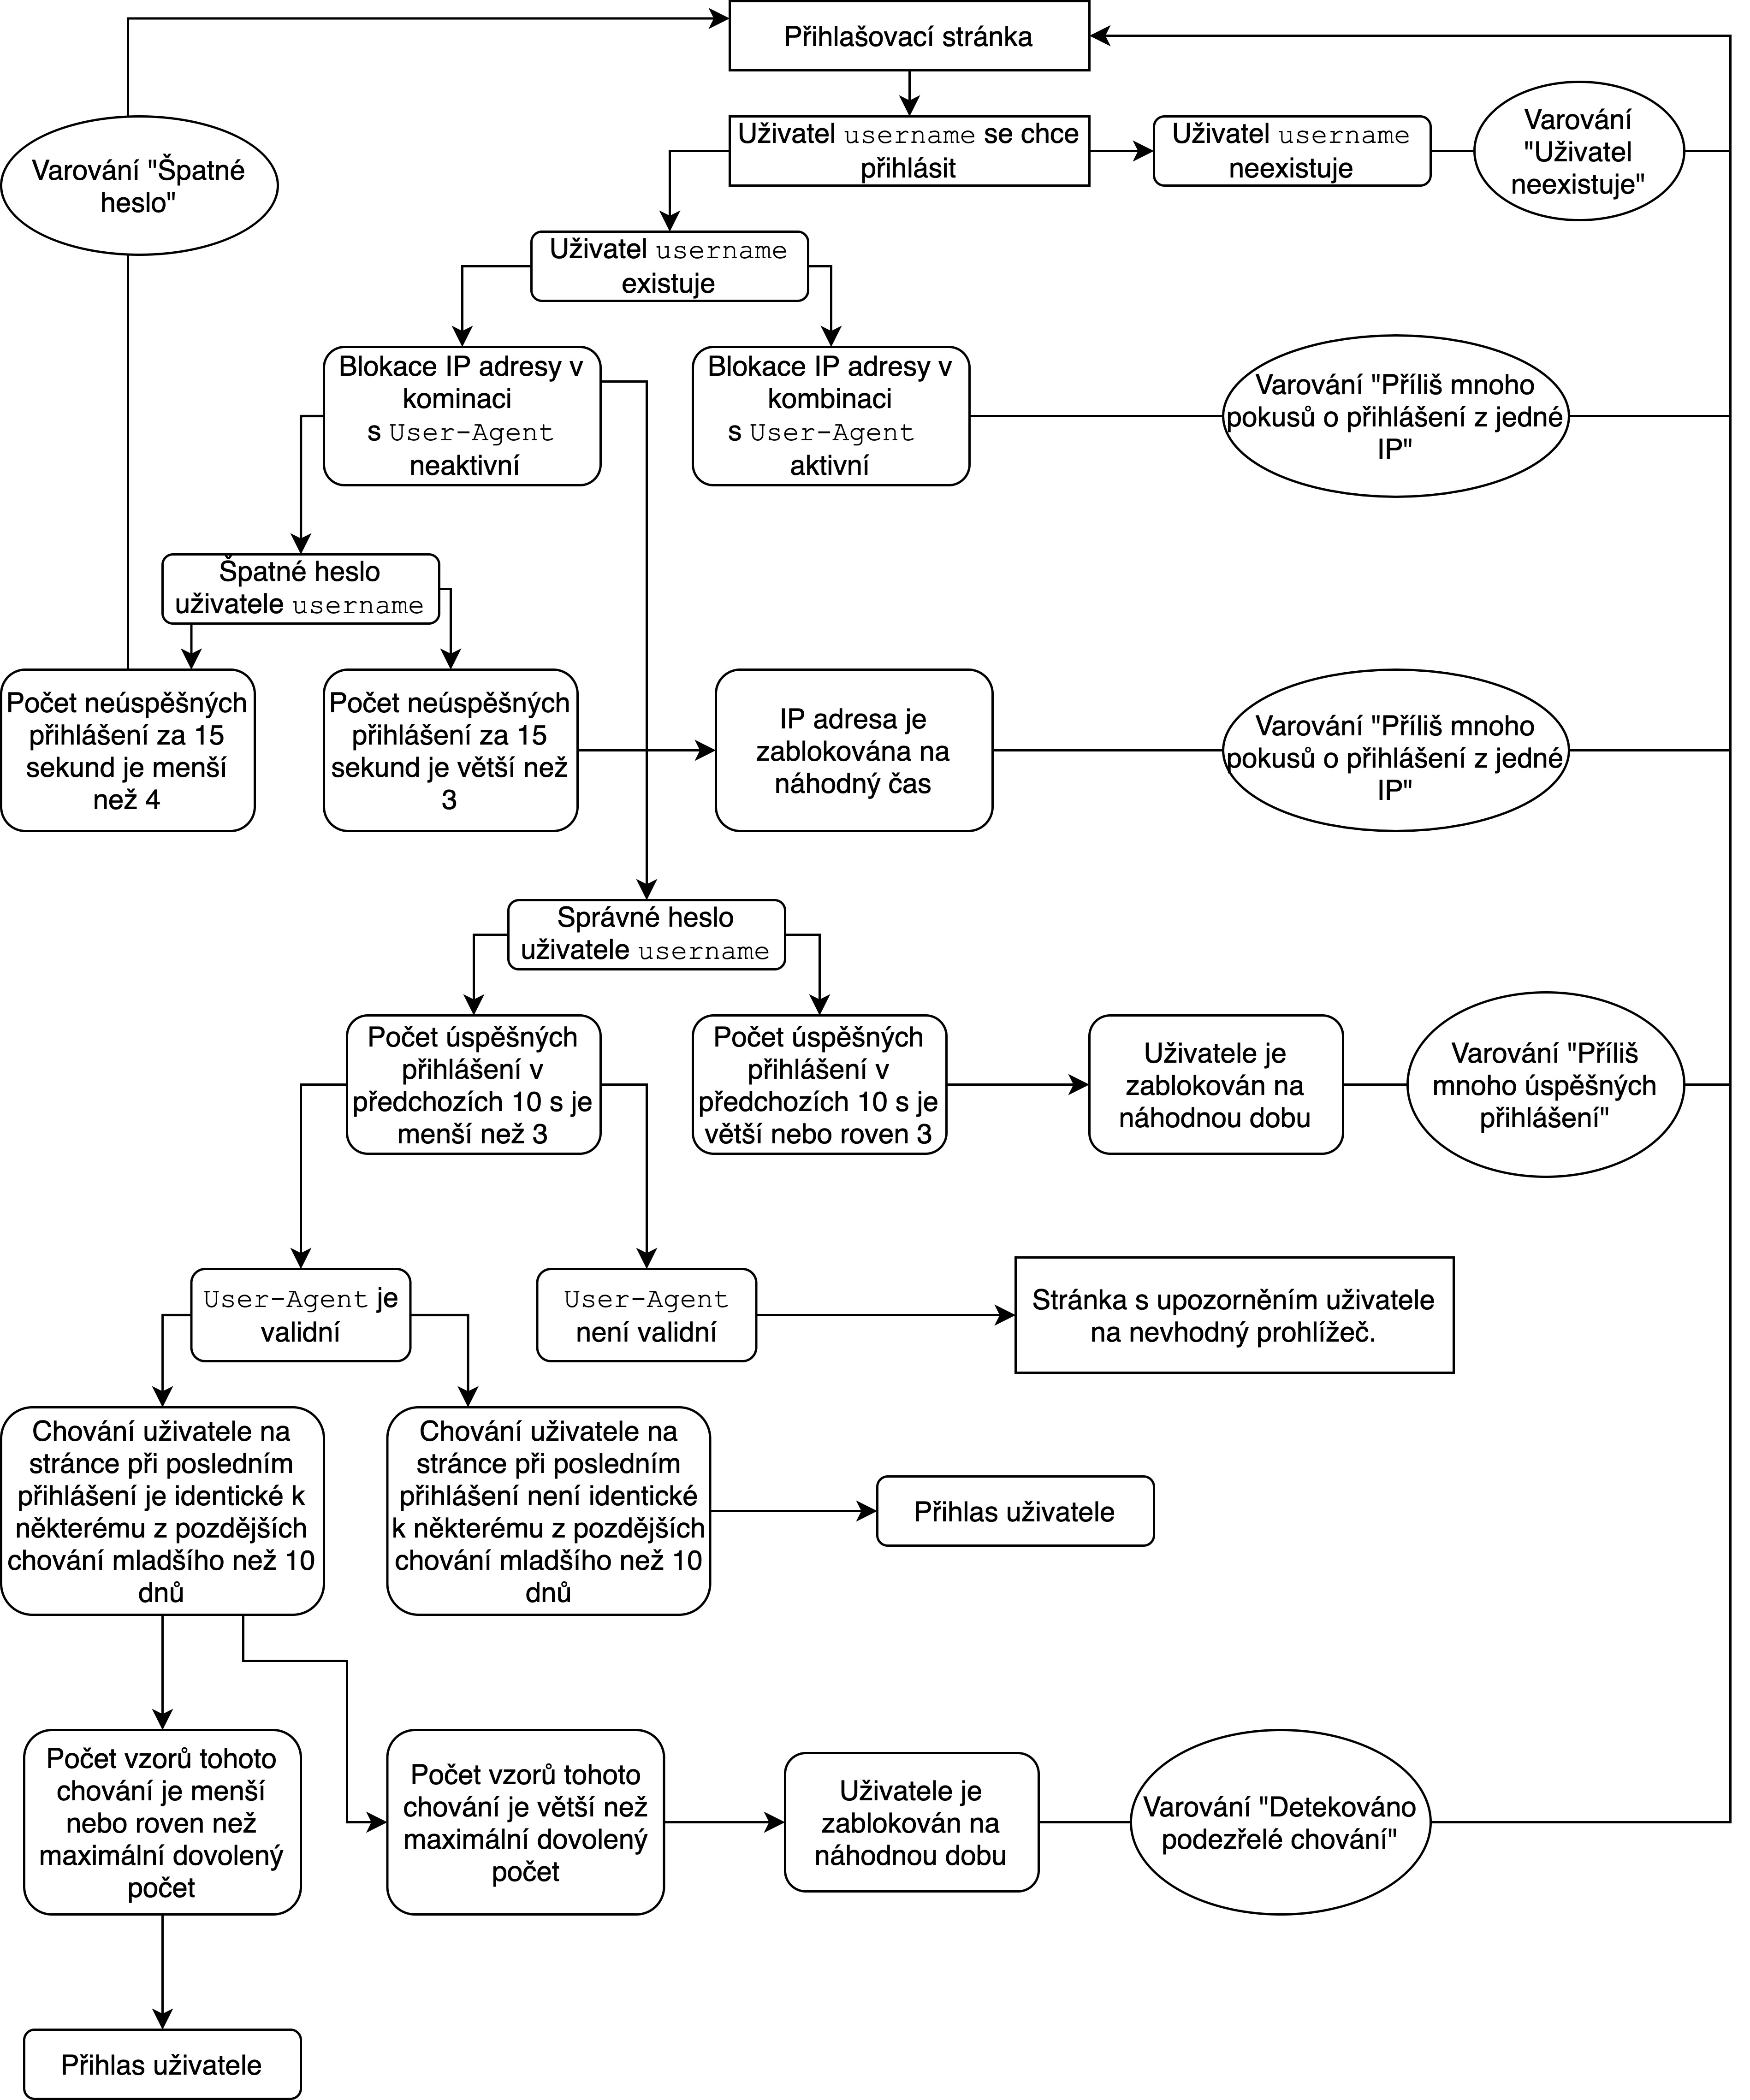
\includegraphics[width=0.9\textwidth]{images/program_scheme.jpg}
	\caption{Pořadí kontrol prováděných aplikačním firewallem při přihlašování uživatele}
	\label{img:program_scheme}
\end{figure}

Sociální síť Socnet funguje jako klasická sociální síť a~normální uživatel by neměl jakkoli poznat, že je jeho aktivita snímána z~důvodu ochrany před automatickým přístupem. Kliknutím na tlačítko 'Přihlásit se' se spustí přihlašovací proces, tedy proběhne kontrola, zda-li není uživatelský provoz podezřelý, a pokud není, vytvoří se nová uživatelská session (session viz~\ref{sec:session}). Seznam kontrol, který probíhají při přihlašování, je uveden v~následujících podsekcích a~probíhá v~tomto pořadí. Kontroly pracují s~logy uživatelů, které se při každé uživatelské akci ukládají do databáze. Všechny časy, které představují intervaly, jsou hodnoty proměnných a dají se nastavit v~souboru \texttt{config.js}. V reálném prostředí by kontroly nebyly tak přísné, ale jejich správné nastavení vyžaduje dlouhodobější časovou analýzu.

\subsection*{Počet neúspěšných přihlášení}
\label{sec:num_of_unsucc_logins}
Jde o~ochranu, která chrání uživatele před prolomením hesla \textit{útokem hrubou silou} (viz~\ref{sec:DoS_force}). Po každém pokusu o~přihlášení se špatným heslem je vytvořen log, jenž je uložen do databáze s~hodnotou \texttt{"action":"BadPassword"}. Pokud se uživatel snaží přihlásit do svého účtu více než $3\times$ za posledních 15~sekund se špatným heslem, je jeho IP adresa v~kombinaci s~\texttt{User-Agent} zablokována na náhodný čas v~intervalu <15,~35> sekund (v~reálné sociální síti by pravděpodobně byla tato doba delší a~uživateli by byl zaslán email). Využívá se kombinace \texttt{User-Agent} a~IP adresy proto, aby zabránilo blokování ostatních uživatelů používajících stejnou IP adresu~--~uživatelský \texttt{User-Agent} v~lozích musí být shodný s~aktuální hodnotou \texttt{User-Agent} (jinými slovy se musí jednat o~přihlášení ze~stejného prohlížeče). Příklad upozornění uživatele o~zablokování IP adresy je vyobrazeno na obrázku~\ref{img:blocked_IP}.

Pokud se uživatel pokusí přihlásit ze~stejného prohlížeče znovu v~tomto intervalu, tak se tento čas do nejbližšího přihlášení \textit{nezmění} ani \textit{není vytvořen žádný log}. 

\begin{figure}[H]
	\centering
	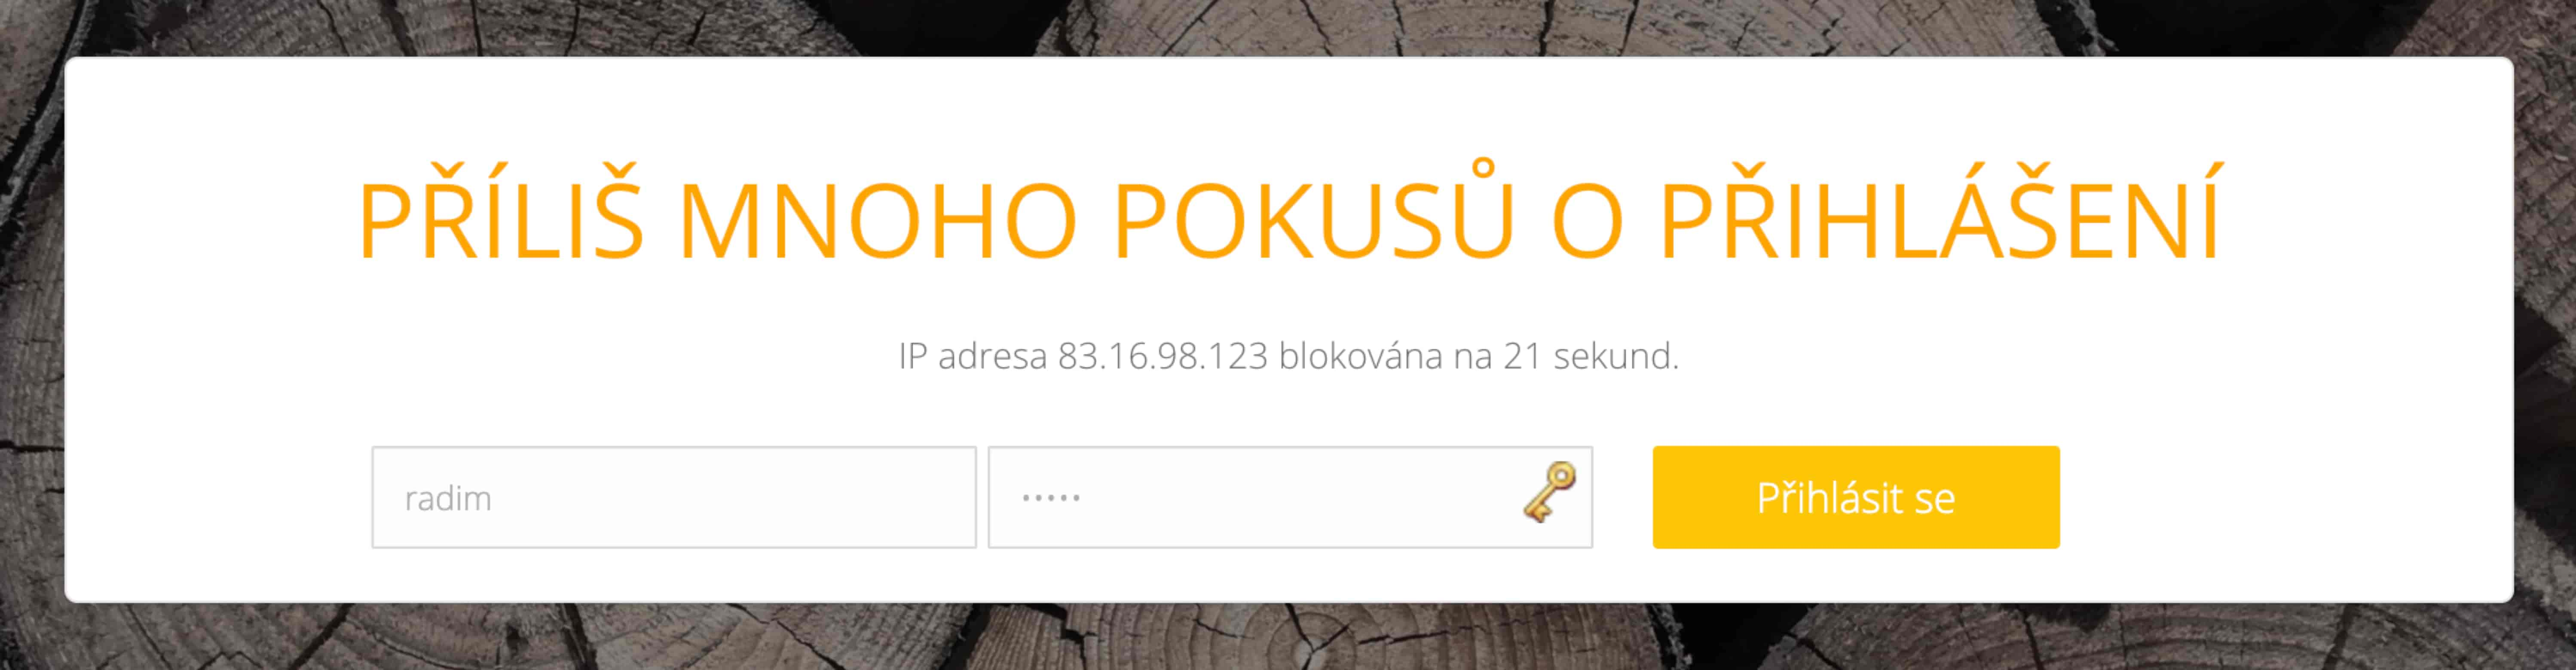
\includegraphics[width=0.8\textwidth]{images/blocked_IP.jpg}
	\caption{Příliš mnoho pokusů o~přihlášení se~špatným heslem}
	\label{img:blocked_IP}
\end{figure}


\subsection*{Počet úspěšných přihlášení}
\label{sec:num_of_succ_logins}
Jde o~ochranu, která zabraňuje více přihlášením v~intervalu 10~sekund na jeden uživatelský účet. Hlavní účel přihlašování se v~krátký časový interval na jeden uživatelský účet je odstavit síť DoS útokem. Jeden reálný uživatel není schopen přihlásit se v~rámci krátkého časového intervalu do svého účtu více než $3\times$, proto je jeho účet zablokován. Každé úspěšné přihlášení do sítě Socnet je zaznamenáno vytvořením logu s~hodnotou \texttt{"action":"login"}. Při přihlašování jsou načteny tyto záznamy mladší než 10~sekund. Pokud je počet těchto logů pro daného uživatele větší než 3, je uživatelský účet zablokován na náhodnou dobu v~intervalu <10,~30> sekund.

V případě, že se uživatel pokusí přihlásit v~tomto intervalu znovu, doba k~nejbližšímu přihlášení se \textit{aktualizuje} na náhodnou dobu v~intervalu <10,~30> sekund a~\textit{není vytvořen žádný log}. Nový čas se generuje z~důvodu aplikace co největší náhodnosti, která je pro automatického robota obtížněji překonatelná. Upozornění o~zablokovaném účtu je zobrazeno na obrázku~\ref{img:too_many_logins}.

\begin{figure}[H]
	\centering
	
\includegraphics[width=0.8\textwidth]{images/too_many_logins.jpg}
	\caption{Příliš mnoho úspěšných přihlášení v~krátkém časovém okamžiku}
	\label{img:too_many_logins}
\end{figure}

\subsection*{Kontrola hodnoty \texttt{User-Agent}}
\label{sec:check_UA}
Hlavička \texttt{User-Agent} obsahuje informace (více viz~\ref{sec:user_agent}) o~uživatelské stanici. Jestliže není tato hodnota korektní, pravděpodobně se jedná o~podezřelý provoz, protože velmi jednoduchý bot tuto hodnotu neuvádí vůbec nebo má takovou hodnotu, kterou server neakceptuje. Aplikační firewall sítě Socnet kontroluje pomocí regulárního výrazu, zda uživatelský \texttt{User-Agent} odpovídá standardnímu tvaru pro hlavičku \texttt{User-Agent} a~zda neobsahuje nepovolené znaky.

Pokud aplikační firewall odhalí neplatný \texttt{User-Agent}, \textit{nepovolí} uživateli přihlásit se z~tohoto prohlížeče. Varovná hláška je vyobrazena na obrázku~\ref{img:bad_user_agent}.

\begin{figure}[H]
	\centering
	
\includegraphics[width=0.8\textwidth]{images/bad_user_agent.jpg}
	\caption{Upozornění Socnetu na nesprávnou hodnotu \texttt{User-Agent}}
	\label{img:bad_user_agent}
\end{figure}

\subsection*{Chování uživatele na sociální síti}
\label{sec:identical_behaviour}
Analýza uživatelského chování je nejpodstatnější a~nejsložitější ochrana sítě Socnet. Snaží se rozpoznávat identické chování uživatele od chvíle, kdy se přihlásí do okamžiku zrušení session, tzn. do odhlášení nebo expirace session. Funguje na principu zaznamenávání aktivity do databáze pomocí logů. Aplikační firewall tedy zaznamenává do databáze okamžik přihlášení uživatele a~dále všechna jeho kliknutí. Log vzniklý kliknutím obsahuje hodnotu \texttt{"action":"click"} a~dále čas kliknutí a~jméno elementu, na který uživatel kliknul. V~okamžiku kliknutí na tlačítko 'Odhlásit se' se zaznamenává poslední log s~hodnotou \texttt{"action":"logout"}. Pokud automaticky expiruje session, nezaznamenává se žádný log.

Každé toto chování je vyhodnoceno jako vzorec chování. Vzorec chování se tedy skládá z~minimálně jedné akce s~hodnotou \texttt{"action":"login"}. Další akce odpovídají jednotlivým kliknutím na stránce a~poslední log zpravidla obsahuje hodnotu \texttt{"action":"logout"}. Vzorec chování je uložen ve formátu JSON, jehož příklad je uveden zde~\ref{json:behaviour_pattern}. 

\begin{figure}[H]
    \centering
    \begin{verbatim}
{   
    "action": ["login", "click", "click", "click", "logout"],
    "element": ["null", "like-post1", "comments1", "like-post2", "logout"],
    "seconds_after_login": [0, 2, 5, 7, 15],
    "last_login": "2021-04-24T17:18:31.932+00:00",
    "userId": "607718ec6a5f38c89e030614",
    "count": 3,
}
    \end{verbatim}
    \caption{Vzorec chování ve formátu JSON}
    \label{json:behaviour_pattern}
\end{figure}
\bigskip

\noindent
Při každém přihlášení se vyhodnocuje \textit{chování odpovídající poslední session} následujícím způsobem:

\begin{enumerate}
  \item Z~databáze se načtou všechny logy odpovídající \textit{poslední session} a~z nich:
  \begin{itemize}
      \item Je vytvořeno pole, do kterého jsou přidány názvy jednotlivých akcí, například \texttt{[login,~click,~logout]}.
      \item Je vytvořeno pole, do kterého jsou přidány časy akcí v~sekundách od přihlášení (zaokrouhleno na celé sekundy) včetně samotné akce přihlášení, například \texttt{[0,~2,~9]}.
      \item Je vytvořeno pole, do kterého se ukládají názvy HTML elementů, na které bylo kliknuto (pro akci \texttt{login} se ukládá hodnota \texttt{null}), například
      \\ \texttt{[null,~like-post1,~logout]}.
      \item Poté se vytvoří příslušný vzorec chování s~těmito hodnotami.
  \end{itemize}
  \item V~databázi se hledá identický vzorec (příklad vzorce chování zde~\ref{json:behaviour_pattern}) chování \textit{ne starší 10~dnů} a~pokud je nalezen, přičte se 1~k počtu opakování vzorců tohoto chování, v~opačném případě se uloží nově vytvořený vzorec a~hodnota \texttt{count} je nastavena na 1. Se vzorcem se dále pracuje v~bodě 3.
  \item Pokud je počet opakování vzorce \texttt{count} větší než povolený počet\footnote{S narůstajícím počtem akcí je méně pravděpodobné, že se vzorec chování bude opakovat a~naopak~--~pokud vzorec obsahuje 2~akce, je více pravděpodobné, že se vzorec zopakuje, proto je počet dovolených opakování vzorce závislý na počtu akcí.} (závislost počtu akcí na povoleném počtu opakování je uvedena v~tabulce~\ref{tab:allowed_num_of_repeatings}), znamená to, že uživatelské chování se za posledních 10 dnů příliš často opakuje, a uživatelský účet je zablokován na náhodný čas v~intervalu <10,~30>~sekund. V~opačném případě je uživatel přihlášen.
  \item Pokud byl uživatel zablokován (nebyl přihlášen), odečte se od počtu opakování \texttt{count} tohoto vzoru 1, aby byla při příštím přihlášení splněna podmínka maximálního počtu opakování vzorce. Uživatel poté musí počkat vygenerovaný náhodný čas, aby se mohl přihlásit~--~varovná hláška je zobrazena na obrázku~\ref{img:bad_behaviour}.
  \item Až náhodný čas blokace uplyne, uživateli bude umožněno se přihlásit, přičemž znovu budou provedeny všechny testy uživatele včetně tohoto testu.
\end{enumerate}

\noindent
Pokud se uživatel v~době své blokace pokusí přihlásit znovu, doba k jeho nejbližšímu přihlášení se aktualizuje na náhodnou dobu v~intervalu <10,~30>~sekund   (podobně jako v~případě vícenásobného úspěšného přihlášení v~krátkém intervalu).

Všechny hodnoty v tabulce~\ref{tab:allowed_num_of_repeatings} jsou pouze orientační a~je vhodné je optimalizovat tak, aby byl \textit{správně odhalen} automatický přístup, ale také tak, aby \textit{nebyl zablokován} normální uživatel.

\begin{table}[ht]
\centering
\label{tab:allowed_num_of_repeatings}
\begin{tabular}{|c|c|}
\hline
\textbf{Počet akcí na stránce} & \textbf{Počet povolených opakování} \\ \hline
2 & 10 \\
3 & 7 \\ 
4 & 5 \\ 
5 & 4 \\ 
6 & 3 \\ 
7~a více & 2 \\ \hline
\end{tabular}
\caption{Počet povolených opakování vzorce vůči počtu akcí}
\end{table}

\begin{figure}[H]
	\centering
	
\includegraphics[width=0.8\textwidth]{images/bad_behaviour.jpg}
	\caption{Upozornění uživatele o~zachyceném podezřelém provozu}
	\label{img:bad_behaviour}
\end{figure}

\section{Testování funkčnosti aplikačního firewallu}
Funkčnost implementovaného aplikačního firewallu byla otestována pomocí nástroje Selenium WebDriver. Testy byly implementovány v~jazyce Python. Hromadné testy byly spouštěny skriptem v~jazyce Bash. To znamená, že každá ochrana proti automatickému přístupu byla odzkoušena samostatným testem. Testy, které byly provedeny, jsou popsány v~podsekcích níže.

\subsection*{Testování nesprávné hodnoty \texttt{User-Agent}}
Hodnota \texttt{User-Agent} prohlížeče, který spouští Selenium, byla nastavena na hodnotu \\ \texttt{False\_user\_agent}. Testované opatření je popsáno v~sekci~\ref{sec:check_UA}. Při použití nevalidní hodnoty \texttt{User-Agent} byl uživatel přesměrován na stránku s~upozorněním přesně podle předpokladu. Aplikační firewall sítě Socnet tento útok \textit{úspěšně odhalil}.

\subsection*{Test odhalení více úspěšných přihlášení}
Test ověřuje, zda dokáže aplikační firewall odhalit více úspěšných přihlášení jednoho uživatele za posledních 10~sekund. Smysl tohoto opatření je popsán v~sekci~\ref{sec:num_of_succ_logins}. Skript byl naprogramován tak, aby spustil okno prohlížeče a~úspěšně se pokusil přihlásit do sociální sítě. Test se skládá ze~2~částí, aby mohl být správně otestován:

\begin{enumerate}
  \item Méně než 6 přihlášení během 10~sekund~--~firewall \textit{nesmí} odhalit podezřelý provoz a~ve všech 5~oknech nechat uživatele úspěšně se přihlásit.
  \item Více než 5 přihlášení během 10~sekund~--~firewall \textit{musí} odhalit podezřelý provoz, tzn.~v~5 oknech nechat uživatele se úspěšně přihlásit a~v~šestém a~ve všech dalších oknech nesmí dovolit uživateli se přihlásit.
\end{enumerate}

\noindent
Tento test probíhal tak, že se v~jednom okamžiku 5$\times$ (pro první část) či 6$\times$ (pro druhou část) spustil Python skript (tzn. otevřelo se okno Google Chrome) a~uživatel se pokusil přihlásit. V~obou částech se aplikační firewall choval přesně podle očekávání: dovolil prvních 5~přihlášení a~šestá a~další přihlášení byla blokována. Poté bylo vyzkoušeno 10~pokusů o~přihlášení ve stejný čas: uživatel se přihlásil úspěšně pouze 5$\times$ a~ostatní pokusy byly zamítnuty. Aplikační firewall \textit{úspěšně prošel} tímto testem.

\subsection*{Test odhalení více neúspěšných přihlášení}
Test ověřuje další funkci aplikačního firewallu popsanou v~sekci~\ref{sec:num_of_unsucc_logins}. Ochrana sítě Socnetu by měla odhalit případy, kdy se uživatel snaží 3$\times$ nebo více \textit{přihlásit se špatným heslem} z~jednoho webového prohlížeče (tzn. z~jedné IP adresy a~prohlížeče s~daným \texttt{User-Agent}). Skript funguje stejně jako v~předchozím testu, ale do pole pro heslo vyplňuje \textit{špatné} heslo. Probíhá více testů pro zjištění správné funkce:

\begin{enumerate}
  \item Méně než 3~neúspěšná přihlášení během 30~sekund z~jednoho prohlížeče~--~firewall \textit{nesmí} zablokovat provoz z~webového prohlížeče.
  \item Více nebo rovno 3~přihlášením během 30~sekund z~jednoho prohlížeče~--~firewall \textit{musí} zablokovat uživatelský webový prohlížeč.
  \item V~době blokace jiného prohlížeče uživatel nesmí poznat, že se někdo pokusil uhádnout jeho heslo~--~firewall \textit{nesmí} uživateli zakázat přihlášení se z~ostatních stanic v~době blokace útočícího prohlížeče\footnote{Klasická sociální síť by však zaslala uživateli email o~zablokování účtu a~pravděpodobně vyžadovala změnu hesla.}
  \item Žádnému uživateli nesmí být umožněno přihlásit se ze zablokovaného prohlížeče.
\end{enumerate}

\noindent
Pro první část se skript v~jednom okamžiku spouštěl 2$\times$ a~ihned poté se uživatel zkoušel přihlásit se \textit{správným heslem} ve stejném prohlížeči, což se mu podařilo. V~druhé části bylo spuštěno 5~oken, ve kterých se uživatel snažil přihlásit se špatným heslem~--~ve dvou oknech byl uživatel upozorněn na špatné heslo a~ve dalších byl upozorněn, že jeho IP~adresa byla zablokována. Třetí část probíhala těsně po skončení druhé části, protože uživateli musí být umožněno se přihlásit z~jiného webového prohlížeče~--~uživatel se úspěšně přihlásil. Čtvrtá část testu probíhala ihned po provedení třetího testu a~výsledek byl, že ze zablokovaného prohlížeče nebylo umožněno přihlásit se jakémukoli uživateli. Všechny čtyři části tohoto testu byly vyhodnoceny jako \textit{úspěšné}.

\subsection*{Test identického opakovaného chování}
Tento test zkouší, zda aplikační firewall dokáže odhalit identické chování uživatele na sociální síti tak, jak je popsáno v~sekci~\ref{sec:identical_behaviour}. Uživatelské chování je dáno posloupností těchto kroků:

\begin{enumerate}
  \item Uživatel se úspěšně přihlásí
  \item Klikne na \textit{To se mi líbí} u~prvního příspěvku
  \item Zobrazí si komentáře u~druhého příspěvku
  \item Odhlásí se
\end{enumerate}

\noindent
Tyto kroky představují \textit{vzorec chování}, který se bude opakovat. Selenium \textit{postupně} spouští okna prohlížeče 8$\times$ za sebou (nikoli v~jeden okamžik jako v~předchozích testech) a~v~každém okně se chová identicky dle naprogramovaného chování. Testuje se, zda aplikační firewall zablokuje uživatele při šestém\footnote{Firewall by měl zablokovat uživatele právě po 5~přihlášeních podle tabulky~\ref{tab:allowed_num_of_repeatings}.} procesu přihlášení. Sedmé přihlášení by mělo proběhnout v~pořádku, ale osmé by mělo být opět zablokováno. Aplikační firewall se zachoval přesně podle předpokladu, test byl tedy vyhodnocen jako \textit{úspěšný}.

\section{Další vývoj a~možná vylepšení}
Navrhovaný aplikační firewall nebere v~potaz aktuální denní čas či pořadí dne v~týdnu. Automatický robot může být však naprogramován tak, že bude přistupovat na sociální síť každé pondělí v~13:00 a~bude provádět určité akce. Jiné akce bude provádět ve středu v~07:15 apod.

Vylepšení, které by pravděpodobně zvýšilo účinnost aplikačního firewallu, je analýza chování v~závislosti na \textit{dni v~týdnu}. To znamená, že v~neděli by se aplikační firewall choval jinak než v~úterý. Tím je myšleno, že by bylo analyzováno chování pro \textit{všechna úterý v~posledních 3 měsících} a~pokud by počet identických chování (hodnota \texttt{count}) překročil určitý počet (tabulka s~povoleným počtem opakujících se chování~\ref{tab:allowed_num_of_repeatings} se může libovolně upravovat), provoz by se zakázal. 

Další věc, jež může zvýšit účinnost ochrany před automatickým přístupem, je \textit{analýza chování v~závislosti na denním času}. V~případě, že se uživatel přihlásí v~14:04, jsou analyzována všechna chování, do kterých se uživatel přihlásil v~době od 14:00 do 14:10 například v~posledních 100~dnech. Samozřejmě je vhodné dobře optimalizovat tabulku s~povoleným počtem opakujících se chování~\ref{tab:allowed_num_of_repeatings}. 

Poslední navrhované vylepšení je \textit{zaokrouhlení časů od přihlášení} provedených akcí. Pokročilí roboti totiž mohou provádět stejné akce na sociální síti za jiný čas. Pokud je tedy pole s~časy vypadá například takto: \texttt{[0, 3, 5, 7, 11]}, může být díky zaokrouhlení vyhodnoceno jako ekvivalentní s~tímto polem: \texttt{[0, 3, 6, 8, 10]}. Rozsah zaokrouhlení lze nastavit téměř libovolně, avšak příliš vysoký rozsah nebude fungovat a~může vyhodnotit normálního uživatele jako robota.

Výše uvedená vylepšení lze různě kombinovat a~optimalizovat. Normální uživatel by však neměl zaznamenat jakýkoliv náznak kontroly před automatickým přístupem. Je tedy třeba tyto ochrany nastavovat s~citem a~je nutné získané výsledky často analyzovat. Jestliže aplikační firewall vyhodnotí 50~\% přístupů jako automatické, je pravděpodobně firewall nastaven špatně.

\chapter{Závěr}
Práce popisuje způsoby, jak se mohou webové stránky bránit automatickému přístupu. Byly uvedeny základy webové komunikace, které jsou nutné pro pochopení problematiky automatického přístupu na web. Síťový firewall byl rozdělen na dvě části~--~\textit{firewally nižších vrstev} a~\textit{aplikační firewall}. Firewally nižších vrstev jsou popsány pouze okrajově, avšak součástí této kapitoly jsou i~možné útoky na tyto vrstvy. Aplikačnímu firewallu je věnována celá kapitola, která obsahuje způsoby, jak se mohou webové servery bránit automatickým robotům.

Další část práce se věnuje metodám, jakými lze automatický přístup implementovat, včetně popisu výhod a~nevýhod každé metody. Mnoho webových serverů má tzv.~\textit{rozhraní API}, přes něž mohou ostatní stanice komunikovat automaticky. Druhým způsobem je \textit{webcraping}, což je snaha simulovat přístup člověka pomocí automatického robota například pro získání dat, která jsou pomocí API nedostupná.

Hlavní cíl práce byla analýza aplikačních firewallů sociálních sítí. V~této práci jsou tyto firewally analyzovány pomocí nástroje Selenium WebDriver, což je nástroj, který se často používá pro účely webscrapingu. Byly analyzovány sítě Facebook, Twitter, LinkedIn a~YouTube. Práce obsahuje tabulky se skutečným chováním uživatelů na sociální síti po jejich přihlášení, což jsou informace, které byly využity při implementaci navrhovaného aplikačního firewallu.

Implementační část, tedy vytvořená sociální síť, se snaží rozlišit robota od člověka. Návrhy implementovaných ochran před automatickými roboty vychází z analýzy aplikačních firewallů reálných sociálních sítí. Pokud robot přistupuje na webovou stránku, bývá jeho chování předem naprogramováno, takže se zpravidla opakuje. Toho využívá navrhnutá detekce botů, která zjišťuje opakované chování, pomocí čehož odhaluje automatický provoz. Byly implementovány i~další způsoby, jak odhalit automatický přístup. V~případě, že aplikační firewall vyhodnotí uživatelský provoz jako automatický, zablokuje uživatele či jeho webový prohlížeč na náhodnou dobu. Všechna navrhovaná opatření se úspěšně podařilo implemenovat a~následně otestovat.

Účelem navrhovaného aplikačního firewallu bylo vylepšit stávající ochrany proti automatickým botům, což může vést k~omezení šíření nežádoucího spamu a~k~lepšímu uživatelskému zážitku na sociální síti.
%===============================================================================

  \fi
  
  % Kompilace po částech (viz výše, nutno odkomentovat)
  % Compilation piecewise (see above, it is necessary to uncomment it)
  %\subfile{projekt-01-uvod-introduction}
  % ...
  %\subfile{chapters/projekt-05-conclusion}


  % Pouzita literatura / Bibliography
  % ----------------------------------------------
\ifslovak
  \makeatletter
  \def\@openbib@code{\addcontentsline{toc}{chapter}{Literatúra}}
  \makeatother
  \bibliographystyle{bib-styles/Pysny/skplain}
\else
  \ifczech
    \makeatletter
    \def\@openbib@code{\addcontentsline{toc}{chapter}{Literatura}}
    \makeatother
    \bibliographystyle{bib-styles/Pysny/czplain}
  \else 
    \makeatletter
    \def\@openbib@code{\addcontentsline{toc}{chapter}{Bibliography}}
    \makeatother
    \bibliographystyle{bib-styles/Pysny/enplain}
  %  \bibliographystyle{alpha}
  \fi
\fi
  \begin{flushleft}
  \bibliography{projekt-20-literatura-bibliography}
  \end{flushleft}

  % vynechani stranky v oboustrannem rezimu
  % Skip the page in the two-sided mode
  \iftwoside
    \cleardoublepage
  \fi

  % Prilohy / Appendices
  % ---------------------------------------------
  \appendix
\ifczech
  \renewcommand{\appendixpagename}{Přílohy}
  \renewcommand{\appendixtocname}{Přílohy}
  \renewcommand{\appendixname}{Příloha}
\fi
\ifslovak
  \renewcommand{\appendixpagename}{Prílohy}
  \renewcommand{\appendixtocname}{Prílohy}
  \renewcommand{\appendixname}{Príloha}
\fi
%  \appendixpage

% vynechani stranky v oboustrannem rezimu
% Skip the page in the two-sided mode
%\iftwoside
%  \cleardoublepage
%\fi
  
\ifslovak
%  \section*{Zoznam príloh}
%  \addcontentsline{toc}{section}{Zoznam príloh}
\else
  \ifczech
%    \section*{Seznam příloh}
%    \addcontentsline{toc}{section}{Seznam příloh}
  \else
%    \section*{List of Appendices}
%    \addcontentsline{toc}{section}{List of Appendices}
  \fi
\fi
  \startcontents[chapters]
  \setlength{\parskip}{0pt} 
  % seznam příloh / list of appendices
  % \printcontents[chapters]{l}{0}{\setcounter{tocdepth}{2}}
  
  \ifODSAZ
    \setlength{\parskip}{0.5\bigskipamount}
  \else
    \setlength{\parskip}{0pt}
  \fi
  
  % vynechani stranky v oboustrannem rezimu
  \iftwoside
    \cleardoublepage
  \fi
  
  % Přílohy / Appendices
  \ifenglish
    \input{projekt-30-prilohy-appendices-en}
  \else
    \chapter{Obsah přiloženého paměťového média}

\setlength{\extrarowheight}{15pt}

\begin{table}[H]
\begin{tabularx}{\linewidth}{
  >{\raggedright\arraybackslash\hsize=.5\hsize}X >{\hsize=1.5\hsize}X
  }

\textbf{/app} & Zdrojové soubory v~jazyce Node.JS včetně samostatného README, který obsahuje popis spuštění, a soubor \texttt{config.js} pro nastavení časových intervalů používaných v práci.\\

\textbf{/selenium\_tests} & Veškeré soubory pro analýzu reálných sociálních sítí (kapitola~\ref{chap:app_firewalls_tests}) a~skripty provádějící testy funkcí implementovaného aplikačního firewallu (kapitola~\ref{chap:proposal_of_solution}). \\

\textbf{/text} & Zdrojové soubory \LaTeX~pro sestavení textu práce. \\

\textbf{text.pdf} & Text práce (odevzdávaná verze). \\

\textbf{text\_tisk.pdf} & Text práce (verze pro tisk). \\
\textbf{README.md} & Popis řešené problematiky a jednotlivých částí práce \\

\end{tabularx}
\end{table}
  \fi
  
  % Kompilace po částech (viz výše, nutno odkomentovat)
  % Compilation piecewise (see above, it is necessary to uncomment it)
  %\subfile{projekt-30-prilohy-appendices}
  
\end{document}
